%!TEX root = thesis.tex

%:-------------------------- Preamble -----------------------

% Three languages are supported, which will be reflected in the logo on the front page. Pass the appropriate language
% specified as a class option to uit-thesis. Passing any other languages supported by babel will result in the default
% language on the frontpage. If no language is passed, the default is selected.
%  - USenglish (default)
%  - norsk
%  - samin
% The frontpage comes in two variants, Master's thesis and PhD. Master is default, use classoption 'phd' for the PhD version.
\documentclass[USenglish]{uit-thesis}
\renewcommand{\bibname}{References}
% Lorem ipsum
\usepackage{lipsum}
\usepackage{appendix}
\usepackage{amsthm}
\usepackage{hyperref}
\usepackage{tikz}
\usepackage{pgf-umlsd}
\usepackage{float}
\usepackage{listings}
\usepackage{caption}
\usepackage{subcaption}
\usepackage{amsmath}
\usepgflibrary{arrows}
\usepackage{listings}
\usepackage{amssymb}
\usepackage{enumitem}  
\usepackage{color, colortbl}
\usepackage[utf8]{inputenc}
\usepackage{tabularx, booktabs}
\usepackage{rotating}
\usepackage{glossaries}
\usepackage{threeparttable}
\usepackage{pdfpages} 


\renewcommand\tabularxcolumn[1]{>{\centering\arraybackslash}m{#1}}
\newcolumntype{Z}[0]{>{\hsize=1.55\hsize}X}%
\newcolumntype{s}[0]{>{\hsize=.6\hsize}X}%
\newcolumntype{n}[0]{>{\centering\arraybackslash\hsize=1.25\hsize}X}%


\newtheorem{defs}{Definition}

\makeglossaries

% Add external glossaryentries

\loadglsentries{acronyms}

\newglossaryentry{thesis}
{
  name=thesis,
  description={
    },
}
\newglossaryentry{lage}
{
  name={long ass glossary entry},
  description={
  },
}

\definecolor{TablesColor}{rgb}{0.75, 0.8, 0.85}
\definecolor{AntPool}{rgb}{1, 0.647059, 0} %orange
\definecolor{F2Pool}{rgb}{0.564706, 0.933333, 0.564706} %lightgreen
\definecolor{BTCC Pool}{rgb}{1, 0.843137, 0} %gold
\definecolor{BitFury}{rgb}{1, 0.627451, 0.478431}	%lightsalmon
\definecolor{BW.COM}{rgb}{0.737255, 0.560784, 0.560784} %rosybrown
\definecolor{SlushPool}{rgb}{0.443137, 0.776471, 0.443137} %sgichartreuse
\definecolor{coral}{rgb}{1, 0.498039, 0.313725}
\definecolor{lightyellow}{rgb}{0.980392, 0.980392, 0.823529}

\newcommand{\listdefinitionname}{My list of definitions}
\newlistof{definition}{def}{\listdefinitionname}
\newcommand{\definition}[1]{%
  \refstepcounter{definition}%
  \par\noindent\textbf{The Definition~\thedefinition. #1}%
  \addcontentsline{def}{definition}
    {\protect\numberline{\thechapter.\thedefinition}#1}\par%
}

\def\bitcoin{\leavevmode\rlap{\hskip.5pt-}B}

\def\bitcoinA{%
	\leavevmode
	\vtop{\offinterlineskip %\bfseries
		\setbox0=\hbox{B}%
		\setbox2=\hbox to\wd0{\hfil\hskip-.03em
			\vrule height .3ex width .15ex\hskip .08em
			\vrule height .3ex width .15ex\hfil}
		\vbox{\copy2\box0}\box2}}

\def\bitcoinB{\leavevmode
	{\setbox0=\hbox{\textsf{B}}%
		\dimen0\ht0 \advance\dimen0 0.2ex
		\ooalign{\hfil \box0\hfil\cr
			\hfil\vrule height \dimen0 depth.2ex\hfil\cr
		}%
	}%
}


\begin{document}
\renewcommand{\bibname}{References}
%:-------------------------- Frontpage ------------------------

% \title{Understanding Digital Currencies and Blockchain}
% \title{How Profitable Coul Be Bitcoin}
% \title{Longitudinal Study On Bitcoin Blockchain}
% \title{How Bitcoin Might Be More Profitable? - A Longitudinal Study On the Bitcoin Blockchain About Problems Concerning Scalability, Performance and Fees.}
\title{Trading Network Performance for Cash in the Bitcoin Blockchain}
\subtitle{A Longitudinal Study on Bitcoin's Scalability, Performance, and Costs}	% Optional
\author{Enrico Tedeschi}
\thesisfaculty{Faculty of Science and Technology \\ Department of Computer Science}
\thesisprogramme{INF-3990 Master Thesis in Computer Science - November 2017}
%\ThesisFrontpageImage{img/}	% Optional
\maketitle

%:-------------------------- Frontmatter -----------------------
\frontmatter

%\begin{dedication}
%Dedication here
%\end{dedication}

%\begin{epigraph}
%\epigraphitem{Simplicity is prerequisite for reliability.}{Edsger Dijkstra}
%\epigraphitem{Beware of bugs in the above code;\\I have only proved it correct, not tried it.}{Donald Knuth}
%\end{epigraph}

\begin{acknowledgement}
	I would like to express my very great
	appreciation to Håvard D.
	Johansen for supervising my thesis and
	for his dedication and help he gave me over
	this year. His devotion and love for his job
	made everything much easier, and every time
	we had a talk, he came up with new brilliant ideas
	and shrewd solutions to our problems that totally
	changed my point of view and made me ponder and
	contemplate. I also
	thank him for introducing me in the Academia
	world and into the iAD research group at UiT.
	
	I want to also thank Professor Dag Johansen
	for being such a good motivator and the
	advice given by him has been vital in building
	this thesis and made me more eager to learn
	about the topic after every discussion.
	His capacity to adapt and find solutions for any
	kind of unexpected changes is admirable,
	I’ve been so inspired by this.
	
	My special thanks are extended to the iDA group
	which included me from the beginning in their
	community and helped me to socialize in
	a foreign country.
	
	And finally, I would love to thank my parents
	that always supported my idea of studying
	abroad and motivated me mentally and economically,
	my girlfriend, my brother and my best friends
	that were always by my side, and at the end
	the city of Tromsø that gave me a pleasant
	and warm welcome, by allowing me to study
	at UiT and work as a northern lights photographer.
	
	All of you have a share in this work, thank you!
	
\end{acknowledgement}

%TODO: SUBSTITUTE ALL THE # WITH CORRECT NUMBERS
\begin{abstract}
\label{sec:abstract}
%TODO: change abstract accordingly to the results

%TODO: Short introduction to blockchain
This thesis describes a longitudinal study of Bitcoin,
the perhaps most popular blockchain based system today.
Public blockchains have emerged as a plausible messaging substrate
for applications that require highly reliable communication.
However, sending messages over existing blockchains can be cumbersome
and costly as miners require payment to establish consensus on the
sequence of messages, since the electricity consumption
needed to run miners is not negligible.
The blockchain protocol requires an always
growing size of the information stored in it so its \emph{scalability} is
the biggest problem. For that reason we decided to
collect and store data locally in our own data structure,
necessary for the analysis,
allowing us to save up to $10$ times the amount of disk space.
Today, systems using the blockchain protocol are emerging,
and cryptocurrencies are a glaring example
of its implementation. Bitcoin
represents the largest cryptocurrency on market,
and it has to face a massive scale due to its popularity,
having in $2012$ about fifty thousands
transaction per day and reaching now,
in $2017$, more than three hundred fifty
thousands of transactions
approved every day.

%TODO: Previous works, problems on blockchain and what we did so far
This massive scale in the system leads to a saturation
of the messaging substrate, hence performance issues.
In this thesis we will focus also on the Bitcoin network
performance, in particular, transaction throughput and
latency.
From $2009$ to $2017$ a lot of analyses on
the blockchain have been performed,
enhancing the considerable change in
the block size limit,
from $256$\,bytes to $1$\,\gls{mb},
as an attempt to overcome scalability problems.
Different papers were published, discussing
whether changing or not the block size limit.
In addition, the Bitcoin price increased
from $\sim$\,$0.7$\,\$ to more than $7.000$\,\$,
making the system even more desirable for
miners, but causing several complications
in the fee and reward mechanism.
We evaluate and discuss possible ways to improve this fee
mechanism in order to guarantee more revenue for miners along
with an user fee optimization.

We finally present our own system for
longitudinal analysis on the Bitcoin blockchain,
\gls{bas}. It generates a dataset
which contains a significant portion of
the whole blockchain, updated on September~$2017$.
We discuss our results and compare them with
other evaluations from past years, considering
three main key points: \emph{scalability},
\emph{performance} and \emph{fees}/\emph{costs}.
We discuss how scalability affects performance,
and how the costs and fees are dependent
from them both.
We want also to take into consideration
the environmental impact of Bitcoin
and how it affects the coming
of new cryptocurrencies.
We evaluate and
propose, using machine learning techniques,
two different cost prediction models that aim to
predict bandwidth for upcoming transactions
according the fee they are willing to pay, and
the expected revenue for miners according to
the time spent mining.
These models can
be used by application to throttle network traffic to optimize
message delivery. We also discuss
whether the block size limit should be increased for a higher
\emph{throughput} or not.
\end{abstract}

\tableofcontents

\listofdefinition

%:-------------------------- Mainmatter -----------------------
\mainmatter
\chapter{Introduction}
\label{chap:introduction}
%TODO: INSERT: Bitcoin has the unintuitive property that while the ownership of money is implicitly anonymous, its flow is globally visible\,\cite{Meiklejohn:2013}.

%TODO: give a short example of previous work, what they did and show that this problem has relevance for this field! works might be: Rizun one, Bohme (longitudinal study of bitcoin transaction fees) and On scaling decentralized blockchain system.

%TODO: Another question we asked ourself for the data is how the various attributes relate to one another, and a quick way to get an idea of pair-wise relationship is to cross-plot the attributes and later interpolate the results.

%TODO: ADJUST INTRODUCTION
In $1964$, Paul Baran\,\cite{Baran1964:ODC}
described the differences
between a centralized, decentralized and distributed
network. Since then, the attention
in developing systems moved from a centralized scheme to a distributed one,
leaving most of the computation to every single processor in the network
rather than a central coordinator.
Such a change might be easy for systems that require little
security, for instance systems that not do require authentication
and authorization.
However, the more secure a system needs to be, the more the decentralization
process might be tricky as it becomes very important to rely on
some trusted central coordinator.
Systems requiring stronger security are the ones that
are related to e-commerce, banking, and trade;
essentially all systems that have to deal with money.

In $1983$, David Chaum introduced the idea of
digital cash\,\cite{chaum83blindsign}. In $1990$ he founded \emph{DigiCash},
an electronic cash company that closed due to bankruptcy in
$1998$. After DigiCash, other systems such as \emph{e-gold} ($1996$) and
\emph{PayPal} ($1998$) emerged. However, systems for digital currency allowed
digital money transfer while they were still relying on a central authority,
hence, they were centralized or decentralized but not distributed.
In $2008$ Satoshi~Nakatomo presented Bitcoin\,\cite{Nakamoto_bitcoin},
the first decentralized digital currency.
Until $2008$ e-commerce relied exclusively on financial institutions
serving as trusted third parties. Those are involved in the electronic
payments process and they have to guarantee consistency of the
transactions and security of data.

Decentralized digital currencies are not
dependent on any trusted third parties and they are built over a
\gls{p2p} network in which every component has the same
privileges. These systems allow money exchange
without a central authority, which means lower fees, no geographical
separation and global trust among users. After Bitcoin,
more decentralized digital currencies emerged, in $2011$ \emph{Litecoin},
originally based on the bitcoin protocol, then in $2013$
Gavin~Wood presented \emph{Ethereum}\,\cite{ethereum} and in
$2014$ \emph{Monero} currency was released.

The transaction ordering is essential in any currency systems,
however, establishing correct order can be problematic in
decentralized cryptocurrency systems as they allow 
arbitrary nodes to join, including nodes that might be malicious.
If arbitrary or Byzantine faults are allowed,
the system might be left in an inconsistent or invalid state\,\cite{Lamport1982}.
The ability to mask Byzantine faults has been implemented in various systems such as
Byzantium\,\cite{Garcia:2011:EMB}, HRDB\,\cite{vandiver2007hrdb} and MITRA\,\cite{Luiz:2014:MBF}.
These protocols guarantee consistency of transactions having
$f$ faulty nodes, with a total of $N$ nodes where $N=2f+1$ or $N=3f+1$.
Fireflies\,\cite{Johansen2015Fireflies} is perhaps the only Byzantine-fault
tolerant membership protocol that can support overlay-network sizes
of the current Bitcoin network. The protocol has also been demonstrated
efficient in distributing large block of date. %TODO: CITE?
However, the suitability of Byzantine consensus to
support cryptocash has yet to be demonstrated.

\section{Blockchains}
\label{sec:blockchains}
To guarantee the ordering of transaction all these
cryptocurrencies rely on the \emph{blockchain} protocol.
The need to tolerate malicious members was the reason for introducing
the blockchain into cryptocurrency systems.
A blockchain is essentially a distributed
database of records or public ledger of all transactions or
digital events that have been executed and
shared among participating parties\,\cite{crosby2016blockchain}.
The fundamental principle  behind the blockchain is that
consensus on transaction ordering is based on 
contributed computational power rather than number of participants. 
The blockchain works by appending transactions into blocks.
Every block is generated after a relevant computation, called
\emph{proof-of-work}, and each new block is
appended to the public ledger of data, the blockchain, having in
that way an ever growing chain of information
containing every transaction ever happened.
Blockchains essentially implements a distributed
consensus protocols that enable a set of untrusted
processes to agree on the content of an append only data structure,
often referred to as ledgers. 
These ledgers are divided into blocks and linked together in sequence by hashes. 
They facilitate transactions between consenting individuals
who would otherwise have no means to trust each other and
deal with geographical separation and interfacing difficulties.
This technology promises a highly resilient and
communication substrate where messages
are potentially kept for a long time.

Besides its use in cryptocurrency, blockchain technology
opens up to several usages in different sectors
as a basis for a tamper proof
audit ledger in eHealth systems\,\cite{Gjerdrum2016},
or to execute decentralized data policies\,\cite{lonet, codecaps},
in addition, it is already
used by NASDAQ in its private socket market. If used in a \gls{p2p}
file sharing network, blockchain removes the need of a centralized
data base. Moreover it allows users to create
tamper-proof digital identities for themselves and it
opens up to usages in several important sectors
such as trading, file storage, and identity management.

There are several limitations in current blockchain technologies.
The most relevant is \emph{scalability}, due to the steady growth of the
ledger of data. It should be also considered that
decentralized cryptocurrencies operate in open (or permissions less) networks
in which the ledger of data could be manipulated from arbitrary adversaries.
With the emerging of cryptocurrencies, smart contracts came out and
they aim to facilitate, verify, or enforce the negotiation
or performance of a contract\,\cite{szabo1996smartcontracts}.
According to Luu et al., $2016$\,\cite{Luu:2016},
security of smart contracts has not received much attention yet.
Since the only part not protected by cryptography
is the \emph{order of transactions}\,\cite{ethereum_white_paper},
an attacker could try to convince the network that a transaction
occurred earlier than another one to gain money.
The security bugs in smart contracts are classified as
\emph{Transaction-Ordering Dependence},
\emph{Timestamp Dependence}, \emph{Mishandled Exceptions}
and \emph{Reentrancy Vulnerability}\,\cite{Luu:2016}.
In this thesis we will not focus on smart contracts but it is
useful to know that in early $2017$ \gls{rsk} project
was launched. \emph{RootStock} is a smart contract
\gls{p2p} platform built on top of the Bitcoin blockchain and
they are also working on Bitcoin scalability\,\cite{rsk}.
In this thesis we refrain from explaining Bitcoin and its
terminology in detail, while we refer to previous
works, studies or technical papers
from Underwood\, and Böhme et al.\cite{Underwood:2016:BBB,
Bohme2015BETG}
or from Nakamoto and
Wood\,\cite{Nakamoto_bitcoin, ethereum_white_paper}.
\section{Problem Statement}
\label{sec:probdefinition}
The most urgent concerns in the blockchains
are related to scalability, performance and
a profit optimization for the participant
in the system.
In $2015$, Möser and Böhme\,\cite{Moser2015} said that
Bitcoin may not be as cheap for consumers as it appears, and
that Bitcoin users are encouraged to pay fees to miners up
to $10$ \gls{usd}cents, per transaction,
irrespectively to the amount paid.
Already in $2015$, Rizun\,\cite{Rizun:2015:blocksizelimit} wrote that
the block size limit was set at one \gls{mb}, corresponding
roughly to three transactions per second. Today
the transaction rate is over three hundred times larger
than when the block size limit was introduced, hence
increasing the block size limit
is now being seriously considered.
In $2016$ Croman et al.\,\cite{croman2016} announced that
the current trend of increasing the
block sizes on Bitcoin portends
a potential problem where the system
will reach its maximum capacity to clear
transactions, probably by $2017$.
These problems need to be taken
into consideration.

%TODO: REVIEW THIS:
In this thesis we propose a longitudinal study on Bitcoin blockchain,
analyzing most recent data.
In particular, we discuss the scalability of the blockchain, how it affects
the throughput, and we present performance observations of the
Bitcoin blockchain, analyzed with a blockchain analytic system developed
for this purpose. We provide detailed insights and analysis of how
the characteristics of Bitcoin, such as fee,
block size, reward to different
miners have changed over time, and provide an
updated view from the one proposed
by Möser and Böhme\,\cite{Moser2015}.
Furthermore, we analyze the
correlation between the fee paid from a transaction
and its \emph{latency}, or the time it takes to 
become visible in the whole network.
Three different models are proposed to describe how applications
should spend money to improve network performance,
this affects average bandwidth available to an application.
By doing transaction-wise and block-wise experiments
and analyses on the Bitcoin blockchain
we state and focus on three major problems:
\begin{enumerate}[noitemsep]
	\item Scalability
	\item Performance
	\item Costs/Fees
\end{enumerate}

\subsection{Scalability}
\label{sec:prob_stat_scalability}
Scalability and network performances are urgent
concerns in existing blockchain-based
cryptocurrencies\,\cite{croman2016}.
According to Buterin et al.\,\cite{ethereum_white_paper},
if Bitcoin would have the same amount of transactions
as a VISA circuit, its blockchain would grow
about $1$\,\gls{mb} every $3$ seconds, $\sim$\,$28$\,\gls{gb} per day,
instead of the actual growth of $\sim$\,$0.12$\,\gls{gb} per day.
In this thesis we discuss how much scalability affects
centralization in the Bitcoin network
and how its impact will be in a couple of years.
Furthermore, with our analysis we aim to study
how this growth is affecting the system's
performance and costs, and how much they
change if the system capacity is filled with
too many transactions to approve.

\subsection{Performance}
Centralized schemes, like VISA, are immediate while having a
throughput of two thousand transactions per second
up to fifty-six thousand transactions per second\,\cite{croman2016}.
It is true that Bitcoin has lower fees than centralized
currency schemes, but these properties
come at a performance and scalability costs.
In the paper from Croman et al.\,\cite{croman2016}, they
claim that Bitcoin achieve a throughput of
$7$ transactions per second constrained by the block
creation time and the block size limit.
In this thesis we want to analyze the network performance
with new data from $2017$ with regards to
throughput and transactional latency to see how
much a possible change in the block size or block creation time
might influence the efficiency of the system.

\subsection{Costs/Fees}
Bitcoin's strength has always been
its lower fees if compared
to centralized systems.
We aim to find out whether this it still true
today or not, if the fees are still
low and the system still that cheap.
The actual costs of the system
have not been extensively studied yet and Bitcoin might
not be as cheap for costumers as it appears.
During our analysis we could observe a remarkable increase
of the fee paid from users. In this thesis we aim
to find and prove the reasons that leaded to this
scenario and they involve also scalability and
performance problems.
Our first concern while studying fees and tolls
is to analyze whether is possible or not
for applications to control available
bandwidth given from the system by paying
higher fees to miners.

\section{Method / Context}
\label{sec:method}
To analyze performance,
make assumptions on scalability and fees in the Bitcoin
network, data need to be retrieved from a source.
We define three different approaches of data retrieval
and all three have their advantages and disadvantages:
\begin{enumerate}
	\item \textbf{Real time analysis:} It might be done by sniffing the traffic
	on the Bitcoin network in order to get real time data.
	For this analysis at least one full operating node
	needs to be implemented in the Bitcoin network.
	Advantages are that, if you set two or more nodes distributed around the world,
	you can get a lot of useful information regarding the inner-node
	communication (otherwise impossible to obtain) and the block
	propagation time plus the orphaning rate in the system. Disadvantages are
	that you need a relevant disk space to download the full ledger of data
	and the set up it extremely time consuming, plus, you have physical
	and geographical limitations
	in order to get up and running multiple nodes
	in different part of the world, without considering
	bandwidth restrictions and electricity
	costs related to it.
	\item \textbf{Historical data retrieval through Bitcoin Core:} Another solution might
	be to use the client app of
	Bitcoin, Bitcoin Core\,\cite{bitcoincore}.
	You can set up your node containing the full ledger
	locally, storing all the necessary data and have a historical view of the
	entire blockchain. Advantages are that you have the whole view of the system.
	Disadvantages are that, this whole view, still does not include the propagation time nor
	any miner's information, having to retrieve these knowledge separately.
	Plus, to set up the full node might take up to $4$ days and the
	disk space required is in the order of hundreds of \gls{gb}.
	\item \textbf{Historical data retrieval through \gls{api}:} Third choice is to build a system
	locally, and use Bitcoin \gls{api}s to gather data and generate information
	using those. Advantages are that you have more flexibility when retrieving data, allowing
	you to store only useful information, saving a considerable disk space, also,
	the blockchain might be stored in intervals, which gives a faster retrieval,
	more disk space saved and still provides enough information to have a whole
	view of the system. Disadvantages are that still you don't have information about
	block propagation time and orphaning rate, and it might be difficult
	to analyze the blockchain in real time.
\end{enumerate}

In this thesis we use method $3$,
as this enables us to analyze a considerable
part of the blockchain with little up-front
investment in computational resources.
A similar methodology was also adapted
in the $2015$ study by
Möser and Böhme\,\cite{Moser2015},
analyzing tips and tolls in the Bitcoin blockchain,
collecting data until $2014$
and then analyzing more than
nine million of transactions.
Since then, the rate of transactions have
risen considerably from
one hundred thousand per day
to three hundred fifty thousand per day,
so the retrieving part turned
out to be more time consuming than expected.
Despite that, we aim to collect even
a larger portion of the blockchain, storing data smartly in a
\emph{data frame}, which allows us to save
up to $10$ times the amount of disk space
the blockchain actually
requires. Then we analyze our collected data
and with \emph{machine learning}
techniques we define models, discuss about
the results and how much they can be
reliable in a future-wise implementation.
In our data structure we store more than
one hundred twenty million of transactions occurred between
April $2013$ and September $2017$.
We used for the information retrieval, \gls{api}s
from \url{blockchain.info},
combined with a \gls{html} parsing on the same
website for the information missing while retrieving data with
Bitcoin's \gls{api}s.
Our assumption is that we can get enough information about the
Bitcoin blockchain by retrieving
and analyzing only a portion
of the blockchain, but having in that way a finer
granularity than data represented on the Bitcoin website.
In that way we aim to gain more information out of it.
Moreover, sampling data from a
single node in the blockchain gives statistics
representative of the whole system.
\section{Outline}
\label{sec:outline}
This chapter gives a briefly introduction about digital currencies,
centralized and decentralized systems, and it talks about the
emerging of cryptocurrencies. It also focuses to give
a short introduction to the blockchain protocol and
why it is so important in systems such as Bitcoin.
Chapter~\ref{chap:techback} helps the reader
to understand decentralized cryptocurrencies,
focusing on mining and proof-of-work concepts.
It also gives an overall view about previous works
and analyses on the Bitcoin blockchain, and it shortly
introduce the reader to machine learning techniques about
big data management.
Chapter~\ref{chap:expsetup} talks about the system
we have developed for the blockchain analysis, it illustrates
its architecture and structure regarding data
retrieval, manipulation and visualization.
Furthermore, assumptions that need to be
proved in this thesis are defined.
In Chapter~\ref{chap:evaluation} we show our results.
We explain the generated plots and prove our assumptions,
thereby we can discuss possible solutions of the problems
raised.
Finally, Chapter~\ref{chap:conclusion} presents
the conclusions and discussions of the overall work,
leading to the future implementations of our system,
further analyses, and studies of Bitcoin.

\chapter{Background}
\label{chap:techback}
This chapter gives an introduction to
blockchain systems, with a particular
focus on Bitcoin. We will briefly explain
the concept of mining and introduce the notion
of payments and fees in the Bitcoin system.
We will describe
how miners profit from mining,
how a user could choose whether including fee or not in its
transactions, and how performance and scalability are
changing the way miners select transactions.
We will also describe some machine learning
techniques and data structures, plus we will take into
consideration the most relevant studies and works
that has been done in the Bitcoin system regarding
scalability, performance and fees.
The list of symbols
used is shown in Appendix~\ref{app:LOS}.
For further detail we refer
to already existing high-level\,\cite{Bohme2015BETG} or
technical\,\cite{ethereum, bitcoinmining,
	bitcoin_blockchain, Rizun:2015:blocksizelimit, Nakamoto_bitcoin,
	ethereum_white_paper} descriptions.

Differences between \emph{centralized}
and \emph{decentralized} digital currencies
are summarized in Table~\ref{tab:centralized_vs_decentralized}.
As mentioned in Chapter~\ref{chap:introduction}, more decentralized
digital currencies are emerging nowadays, and they aim
to facilitate transactions between consenting individuals who would otherwise
have no means to trust each other and deal with geographical separation and 
interfacing difficulties.
According to Nakamoto\,\cite{Nakamoto_bitcoin} an electronic coin is defined as
follows:
\definition{An \emph{eletronic coin} is a chain of digital signatures.
	Each owner transfers the coin to the next by digitally signing a hash of
	the previous transaction and the public key of the next owner and adding
	these to the end of the coin.}
Transactions are registered in \emph{blocks}, and all these systems use the
\emph{blockchain} technology to maintain a serial order of them.
The blockchain is a consensus protocol that users run to maintain and secure a
shared ledger of data and it is formed of all blocks, ordered by time and linked
between each other with the \emph{previous block} attribute. A transaction is approved
only when it is included in a block, and the miner including this transaction is
the one who has first
solved the \emph{proof-of-work}. Difficulty of proof-of-work is increased
according to keep an average $\mathcal{T}$ of $10$\,minutes.
\begin{table}
	\caption{Centralized vs Decentralized digital currencies}
	\label{tab:centralized_vs_decentralized}
	\centering 
	\begin{tabular}{|p{5.8cm}|p{5.8cm}|}\hline
		\textbf{Centralized}&\textbf{Decentralized}\\
		\hline
		Under the control of a central authority & Requires
		consensus among users to make changes\\
		\hline
		Users depend on the control given from the
		\gls{ca} & Users have full control over their assets/data\\
		\hline
		No need to enforce cryptography or to create keys & User’s data is uniquely identified by their private key \\
		\hline
		Only users allowed by \gls{ca} can participate & Anyone can join and use the ledger \\
		\hline
		Historic transactions can be changed by the \gls{ca} &
		Historic transactions are unalterable and permanent\\
		\hline
		Can be run very efficiently using relational
		databases that fit the need of the applications & Inefficient
		for the cost of mining \\
		\hline		
	\end{tabular}
\end{table}

\section{Mining}
\label{sec:mining}
In a decentralized cryptocurrency network,
transactions need to be approved by all the
participant before being validated and confirmed.
This validation requires high computational
time and it is expensive in matter of
electricity and resources used.

\definition{\emph{Mining} is how transactions are validated and confirmed by the network.}

To validate and confirm transactions, the network needs \emph{miners}.
According to the Bitcoin miner
document\,\cite{bitcoinmining_process}, Bitcoin miners
create new blocks from solving a proof-of-work
problem that is chained through
cryptographic proof of the previous block.
The work and the effort spent to create new blocks
is often referred to as mining\,\cite{bitcoinmining_process}.
The mining process involves identifying a value
that when hashed twice with SHA-256, begins
with a number of zero bits. If the amount
of zeros needed for the creation
is raised, the average work required
increases exponentially, while a hash can always be
verified by executing a single round of
double SHA-256\,\cite{bitcoinmining_process, sha}.
Each miner chooses whether to include a transaction into a block or not,
and we believe that nowadays this inclusion strongly depends on
the fee that this transaction has to offer.
The first miner who solves the proof-of-work gains the sum
of the fees ($t_f$) offered by each transaction included in the block,
$M$, plus the block reward, $R$, which
is now set to $12.5$\,\bitcoinA.
When a new block is mined, that information
is spread through the whole network and
if the solution is propagated to $50\% + 1$
of the nodes in the system,
the block is validated and all the
transactions in it are accepted and confirmed.
Finally, miners in the network express their acceptance by
starting to work on the next block,
incorporating the hash of the newly accepted one.

\subsection{Proof-of-Work}
\label{sec:proof-of-work}
Karpel\`{e}s et al. define the proof-of-work as follows\,\cite{proof-of-work}:
\definition{\emph{Proof-of-work} is a piece of data which is difficult
	(costly and time-consuming) to produce but easy for others to verify and
	which satisfies certain requirements.}

Mining a block is difficult because the SHA-256\,\cite{sha} hash of a block's header
must be lower or equal to a certain \emph{target value} in order for the
block to be accepted by the network.
Producing proof-of-work is a random process with low probability
of hitting the target value,
so that a lot of trial and error is required on average before a valid
proof-of-work is generated. For example, Hashcash is a
proof-of-work system used to limit email spam and
denial-of-service attack and recently has become known
for its use in Bitcoin and other cryptocurrencies as part
of the mining algorithm\,\cite{Back02hashcash}.

\begin{figure}[h]
	\centering
	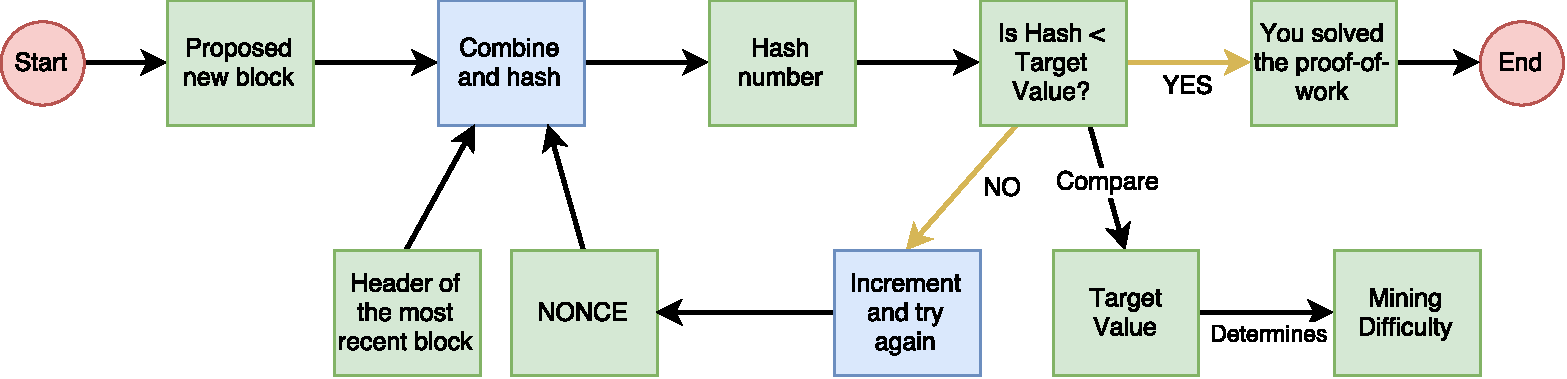
\includegraphics[width=1\textwidth]{img/proof-of-work-schema}
	\caption{Diagram that shows how proof-of-work works.}
	\label{fig:proof-of-work-schema}
\end{figure}

Proof-of-work is a part of the mining process and a valid
proof-of-work is determined by incrementing
a nonce until a value is found that gives the block's
hash the required number of leading zero bits.
Once the hashing has produced a
valid result, the block is immutable and
cannot be changed without
rebuilding a chain bigger than
the original.
As later blocks are appended to the chain,
the work to change the block would include redoing the work for
each subsequent block\,\cite{bitcoinmining_process}.
The best chain is the longest one, so is the one that requires the greatest
effort to produce, and majority consensus in Bitcoin
is represented by this chain. In this way if the
majority of the computing power
is controlled by honest nodes, the honest
chain will grow fastest and outpace any competing chains.
Diagram in  Figure~\ref{fig:proof-of-work-schema} represents
how the proof-of-work is performed, and it
is inspired to the model presented
in \url{bitcoinmining.com}\,\cite{bitcoinmining}.

\subsection{Miners \& Mining Pools}
\label{sec:miner}
With paper money, a government decides when
to print and distribute money. Bitcoin does not
have a central government and
it uses a special software to solve math problems
to get a certain amount of coins in exchange.
This provides a smart way to issue the currency.

\definition{A \emph{miner} is a computer
	specifically designed to solve problems according to the
	proof-of-work algorithm and
	they are required to approve transactions.}

Since miners are required to approve
transactions, more miners mean a more
secure network.
To become a Bitcoin miner nowadays, you
need to buy highly specified chips called
\gls{asic}. Information about this
hardware can be found at
\url{bitcoinmining.com}\,\cite{bitcoinmining}.
In the early days of Bitcoin ($2009$-$2013$)
it was possible to mine with your commodity hardware
or high speed video processor card.
Today that is no longer possible since custom
Bitcoin \gls{asic} chips offer performance
up to $100$ times the capability of older
systems\,\cite{bitcoinmining}. Another reason is
that mining pools became more prevalent,
yielding a constant growth of the \emph{mining difficulty}.

\definition{A \emph{pooled mining} combines the work of many miners
	toward a common goal.}

Pools of miners or mining pools
find solutions faster than individual members and each
miner is rewarded proportionally with the amount of work it provides.
Mining is an important and integral part of Bitcoin that ensures \emph{fairness}
while keeping the Bitcoin network \emph{stable},
\emph{safe} and \emph{secure}\,\cite{bitcoinmining}.

\section{Reward \& Fee}
\label{sec:bitcoinfee}
Miners generate new blocks by appending
transactions to them. Every miner has a \emph{mempool}, $\mathcal{N}$,
containing the new, unapproved, $n$ transactions, and they
get compensated for mining with a revenue $\langle V \rangle = R + M$,
where $M$ is the sum of transaction fees in the block and
$R$ is the block reward, which is now set at $12.5$\,\bitcoinA.
Miners are free to choose
whether to accept or refuse a certain transaction $t\in\mathcal{N}$.
Competitive miners will include transactions as long as the fee exceeds
the marginal cost of inclusion. Production costs are fixed
per block (but may vary between miners depending on access to
technology and energy cooling) and the protocol
defines a maximum block size $Q$.
Because of that, the marginal cost of inclusion is zero if there are
fewer unconfirmed transactions than the capacity left in the block.
Competitive miners make positive expected profits only if transactions
compete for space in the blockchain. Houy\,\cite{houy2014EOBTF}
argues that a maximum block size is necessary for the stability of Bitcoin.
However in that way big mining pools might take advantage from less competition,
having a centralization problem, since a transaction is willing to
compete only if the capacity is reached.
In that way if the system never reaches the capacity, raising the fee
will not be helpful at all. Before $2015$, transactions almost
never required to compete for space in blocks, since the demand
was less then the offer, but nowadays we have a totally different
scenario. 
In $2012$, the number of transactions confirmed per day
reached peaks of fifty thousand, with an average of
fifteen thousand transactions per day\,\cite{bitcoin_blockchain}.
Today we have an average of two hundred fifty thousand
transactions approved every day, with peaks of three hundred
and fifty thousand.
Because of throughput
limitations in the system, caused by the block size limit, $Q$,
set at $1$\,\gls{mb}
and the average block creation
time, $\mathcal{T}$,
set at $10$\,minutes, with
such big scale of transactions
that need to be approved every day,
miners could start to choose transactions with a higher
fee density $\rho$, or simply transactions
that are willing to offer a higher fee
rather than $0$-fee transactions.
The fact that the reward $R$ has a $50\%$ reduction every
two hundred thousand blocks creates the need of a market
mechanism to find the price
of Bitcoin transactions.

\section{Previous Works}
\label{sec:relatedworks}
The main problems analyzed in the past years
concerning the Bitcoin blockchain were related
to scalability\,\cite{Rizun:2015:blocksizelimit, croman2016},
performance\,\cite{croman2016, Decker2013IPBN} and
costs/fees\,\cite{Rizun:2015:blocksizelimit, Moser2015}.
Already in $2014$ researchers believed that
these "fees" users were paying to miners
were supposed to substitute miners' minting
reward in the long run\,\cite{Moser2015}.
In $2015$ discussions about how a rational
Bitcoin miner should select transactions from
his node mempool raised, and ideas about
maximizing miners' profit when creating a new block
emerged. Equations that aim to calculate the
cost of mining $\langle C \rangle$
and the miner's profit $\langle \Pi \rangle$ were
presented by Rizun\,\cite{Rizun:2015:blocksizelimit} and
the concept of \emph{orphaning} was introduced. as well
Scalability is still a huge concern,
causing relevant bottlenecks in Bitcoin which
limits the ability of the current \gls{p2p}
overlay network to support substantially higher
throughputs and lower latencies\,\cite{croman2016}.

\subsection{A Transaction Fee Market Exists Without a Block Size Limit}
A pressing concern exists over
the ramifications of changing (or not)
a Bitcoin protocol rule called
\emph{block size limit}. This rule sets an
upper bound on the network's
transactional capacity, or \emph{throughput} ($\gamma$).
The limit is currently set to $1$\,\gls{mb},
corresponding roughly to three transactions
per second. This limit set by the
blockchain protocol, allow miners
to include up to $1$\,\gls{mb} of
transactions selected from
their mempools. When this limit
was set, it was over eight hundred times
greater than what was required.
However in $2015$, blocks
were filled near the capacity and users
experienced delays. In $2015$
the transaction rate was over
three hundred times larger
than when the block size limit was introduced.
To improve performance the block 
size limit should be raised,
but in that way transactions will not
compete anymore for space in the block,
creating an unhealthy transaction fee
market. Miners should then include
transactions in a manner that maximizes
their expected profit\,\cite{Rizun:2015:blocksizelimit}.
For that reason \emph{Miner's Profit Equation},
\emph{Mempool Demand Curve}, \emph{Block
Space Supply Curve} and the concept of
fee density were introduced.
Every time a block is mined, the miner expects to
generate a revenue $\langle V \rangle$
at hashing cost $\langle C \rangle$, yielding
a profit $\langle \Pi \rangle$ as follows:
\begin{equation}
\label{eq:minerprofit}
\langle \Pi \rangle = \langle V\rangle - \langle C\rangle.
\end{equation}
where the hashing cost is represented by:
\begin{equation}
\label{eq:hashingcost}
\langle C\rangle = \eta h\mathcal{T}.
\end{equation}
So the hashing cost $\langle C\rangle$ is
directly dependent on the miner's individual hash rate, $h$,
the cost per hash, $\eta$, and the creation time, $\mathcal{T}$.
The revenue $\langle V\rangle$
is calculated with the amount he would earn if he won
the block (reward plus fees, $R + M$) multiplied by his probability of
winning (ratio between miner's hash rate, $h$, and
hash rate of the Bitcoin network, $H$), considering also the orphaning
rate presented in Equation~\ref{eq:orphaning}.
\definition{A block $B_1$ generated at a timestamp $t_1$
	is \emph{orphan} if it does not
	get approved by the network because another block $B_2$ with
a greater timestamp $t_2 > t_1$ which propagates faster, gets approved instead.}
So the expected revenue is shown in Equation~\ref{eq:expectedrevenue}:
\begin{equation}
\label{eq:expectedrevenue}
\langle V\rangle = \left(R + M\right)\frac{h}{H}\left(1 - \mathbb{P}_{orphan}\right).
\end{equation}
Where $\mathbb{P}_{orphan}$
increases with the amount of time a block takes
to propagate through network. If $\tau$ is
the block propagation time, the
probability of orphaning is defined as:
\begin{equation}
\label{eq:orphaning}
\mathbb{P}_{orphan} = 1 - e^{-\frac{\tau}{\mathcal{T}}}.
\end{equation}
We can now define the miner profit equation as follows:
\begin{equation}
\label{eq:minerprofiteq}
\langle \Pi \rangle = (R + M)\frac{h}{H} e^{-\frac{\tau}{\mathcal{T}}} -\eta h\mathcal{T}.
\end{equation}
A \emph{rational miner} selects which
transactions to include in his block in a manner that maximizes
the expectation value of his profit. This
selection is explained with the Mempool Demand Curve
and the Block Space Supply Curve.
According to the size limit, a block can select a $b \leq n$
transactions from $\mathcal{N}$ to create a
new block $\mathcal{B} \subset \mathcal{N}$.


Studies on inclusion came to the
conclusion that a block first includes transactions
with a higher \emph{fee density}, $\rho$,
which is the ratio between
the \emph{transaction fee}, $t_f$, and
the \emph{transaction size}, $t_q$.
To construct the mempool demand
curve, the mempool must be sorted from
greatest fee density to least and its
formula is shown in Equation~\ref{eq:memdemandcurve}.
\begin{equation}
\label{eq:memdemandcurve}
M_{demand}(b) \equiv \sum_{i=1}^{b} t_{fi},
\end{equation}
and the sum of each transaction size in bytes, form the
block size $Q$:
\begin{equation}
\label{eq:transactionsize}
Q(b) \equiv \sum_{i = 1}^{b} t_{qi}.
\end{equation}
The mempool demand curve represents then
the maximum fee, $M_{demand}(b)$
a miner can claim by producing
a given quantity $Q(b)$ of block space.
The size of the block a miner elects to
produce controls the fees he attempts to claim, $M(Q)$,
and the propagation time he chooses to risk, $\tau(Q)$.
The block space supply curve represents
the fees a miner requires to cover the additional cost of
supplying block space $Q$. This cost grows
exponentially with the propagation time. The equation which
represents this curve is the one shown below:
\begin{equation}
\label{eq:blockspacesupply}
M_{supply}(Q) = R\left(e^{\frac{\Delta \tau (Q)}{\mathcal{T}}} - 1\right),
\end{equation}
where $\Delta \tau (Q) \equiv \tau(Q) - \tau(0)$.
In order to have a transaction fee market
without a block size limit, to maximize his profit,
the miner constructs a mempool
demand curve and a space supply curve.
The block size $Q^*$ where the miner's surplus,
$M_{demand} - M_{supply}$, is largest represents
the point of maximum profit.

\subsection{Trends, Tips and Tolls} %TODO: BRAKE IT UP
The Bitcoin protocol supports direct payments
from transaction partners to miners,
also called \emph{fees} ($t_f$). Acknowledging their
role in stabilizing of the system, the right level of
transaction fees is a hot topic of normative debate.
The actual costs of the system are
not extensively studied and
Bitcoin may not be as cheap for
consumers as it appears.
The definition of transaction fee is encoded
as difference between the sum of all inputs
and the sum of all outputs
of a transaction (Equation~\ref{eq:txfee}).
Previous analyses on the Bitcoin blockchain
such as the one presented by
Möser and Böhme in $2015$\,\cite{Moser2015},
show that transaction fees are lower than $0.1\%$ of
the transmitted value, which
is significantly below the fees charged
by conventional payment systems, and at the time
of analysis the hard size limit
did not (yet) significantly drive
the level of transaction fees. However
trends for the fees paid per transaction
over time noticeably changed. The trend
of $0$-fee transactions had a drop
after April $2012$ leaving space to
$0.0005$\,\bitcoinA~fee until May $2013$.
After that, until the beginning of $2015$
the trend for fees was of $0.0001$\,\bitcoinA~and
$0.0002$\,\bitcoinA, with peaks of
$0.001$\,\bitcoinA. Generally,
there seem to be two main
reasons for the shift in trends:
changes to the Bitcoin reference implementation
and actions by large intermediaries in the ecosystem.
The emergence of $0.0005$\,\bitcoinA~fees
in June $2011$ can be mapped to the release of version $0.3.23$
of the Bitcoin Core client, which reduced the default transaction fee
from $0.01$\,\bitcoinA~to $0.0005$\,\bitcoinA. The raise of these
last transaction fees in the second quarter of $2012$ was probably
due to the launch of the gambling website \emph{SatoshiDice}\,\cite{satoshidice}.
In May $2013$, version $0.8.2$ of Bitcoin Core was released.
In the past years, during a period between
$2011$ and $2015$ there was a small share of
transactions that did not offer fee to miners,
most of them offered default fee amount but some of them
were even willing to pay a higher fee, a tip. A plausible reason
is that paying more fee led to a faster confirmation.
Analysis on the blockchain in $2015$\,\cite{Moser2015}
state that half of all $0$-fee transactions
had to wait more than $20$\,minuets for their first confirmation.
In contrast to that, paying a $0.0005$\,\bitcoinA~fee lead to an
inclusion into a block in half the time. $10\%$ of all $0$-fee
transactions took almost $4$\,hours to confirm, in contrast
to $40$\,minutes for transactions paying
a $0.0005$\,\bitcoinA~fee. The difference
between paying $0.0005$\,\bitcoinA~or
$0.001$\,\bitcoinA~fee is not as pronounced, but the difference
in medians are still statistically and economically significant.
Analysis on pool behavior regarding a possible systematic
exclusion of $0$-fee transactions has been done.
Shares have shifted between pools quite extensively.
In $2013$, BTC Guild had a market share of up to $40\%$,
in $2014$ both GHash.IO and Discus Fish ousted this pool.
Also, the share of other pools has rose in $2014$. Previous
incumbents like Slush or $50$BTC have lost popularity.
Possible reasons include economic and technical factors,
like pool fees, service availability, or robustness against
attacks. Given the dominance of a few mining pools, evaluations
whether some pools systematically enforce fees has been made.
The results show that two pools, Discus Fish and Eligius,
have a considerably higher share of blocks without any
$0$-fee transaction, with $30.6\%$ for Eligius and $62.5\%$
for Discus Fish, in contrast to an average of $14.4\%$.
Other than that though, there is no clear evidence for
enforcement of strictly positive transactions fees.

\subsection{Bitcoin Performance Limitation}
Can decentralized blockchains be scaled up to match the performance
of a mainstream payment processor? What does it take
to get there?
In $2016$ the Bitcoin blockchain took $10$\,minutes or longer
to confirm transactions, achieving $7$ transactions per second maximum
throughput. Visa credit card confirms a transaction within seconds
and processes two thousand transactions per second on average with peaks
of fifty-six thousand transactions per second.
Bitcoin community has put forth various proposals to modify
the key systems parameters of block size and block interval.
Anyway, Croman et al. state that such scaling by reparametrization
can achieve only limited benefits\,\cite{croman2016}.
This is because because Bitcoin
generates a lot of network traffic, due to its
decentralization, this leads to have a lot of peers in the network
and they all have to interact. To ensure that most
of the nodes in the overlay network have sufficient
throughput we follow two guidelines:
\begin{itemize}[noitemsep]
	\item \textbf{Throughput limit.} The block size should not exceed $4$\,\gls{mb}
	given $10$\,minutes average block interval. Corresponding to maximum
	$27$ transactions per second.
	\item \textbf{Latency limit.} The block interval should not be smaller
	than $12$\,seconds.
\end{itemize}
The maximum throughput of $3$-$7$ transactions per second is
a number constrained by the $1$\,\gls{mb} block size $Q$ and the
$10$\,minutes creation time $\mathcal{T}$.
About the propagation time $\tau$, measured
in $2016$\,\cite{croman2016} shows that
$10\%$, $50\%$ and $90\%$ block
propagation times are $0.8$\,seconds,
$8.7$\,seconds and $79$\,seconds respectively,
with an average block size of $540$\,\gls{kb}.
Projecting to a $1$\,\gls{mb} block size, $\tau$
would be $2.4$\,min, $15.7$\,sec, and $1.5$\,sec respectively.
In that way an effective throughput on the network
could be calculated as follows:
\[
\text{X\% effective throughput} = Q / (\text{X\% block propagation delay}).
\]
Having with $\text{X} = 50\%$, an effective throughput of $496$\,Kbps,
equals to $248$\,tx/sec, and with $\text{X} = 90\%$, an effective throughput
of $55$\,Kbps, equals to $26$\,tx/sec.
It follows that $Q$, and interval $\mathcal{T}$,
must satisfy Equation~\ref{eq:effectivethroughput}:
\begin{equation}
\label{eq:effectivethroughput}
\frac{Q}{\text{X\% effective throughput}} < \mathcal{T}
\end{equation}
Consequently, for a $10$\,minute (or shorter) block interval,
the block size should not exceed $4$\,\gls{mb} for $\text{X} = 90\%$;
and $38$\,\gls{mb} for $\text{X} = 50\%$, corresponding to a throughput
of at most $27$ transactions per second.
To improve the system's latency it could be enough
to reduce the block interval. To maintain effective
throughput would also require a reduction in the
block size. Propagating a block smaller than $80$\,\gls{kb} would
not make full use of the network's bandwidth, as latency would
still be a significant factor in the block's propagation time.
Propagating an $80$\,\gls{kb} block to $90\%$ of the nodes would
take roughly $12$\,seconds. In conclusion, to retain at least $90\%$
effective throughput and fully utilize the bandwidth of the network,
the block interval should not be smaller than $12$\,seconds.

\section{Machine Learning}
\label{sec:machinelearning}
When a new node joins the Bitcoin network, it has to download
all the useful information to process transactions and
verify them. This information consist of a relevant quantity
of data, nowadays $\sim$\,$125$\,\gls{gb}, and it grows
continuously over time.
A full node might require more than four days to 
download the entire ledger. Once all the data are
collected, is necessary to implement a way to
store them and to get the right information
out of them. Many data structures allow
the storing of big datasets, and
several machine learning
techniques grant to infer more information
out of them. While applying machine
learning techniques to big datasets
might be recommended to use
data structures such as \emph{trees}
or \emph{data frames} which are
more likely to be used in machine learning
algorithms.

\subsection{Training Dataset}
\label{sec:trainingdataset}
Having a huge dataset implies having a big amount
of data with different types of attributes.
These attributes might have
\emph{numerical} or \emph{categorical} values. 
\begin{description}[leftmargin=!, labelwidth=\widthof{\bfseries -Categorical- }, noitemsep]
	\item [Numerical:] Data that can be measured, quantified. For example
	the fee $t_f$ paid to a miner in \gls{btc}.
	\item [Categorical:]Data which represent characteristics. For
	example the name of the miners in the Bitcoin system.
\end{description}
These data might be saved in a data structure such as a data frame,
having a sample for each row and different attributes of that particular
sample on every column.
Once data are collected, they might be trained
to create predicting
models or other useful material.
Training and predicting models involve
different types of variables:
\begin{description}[leftmargin=!, labelwidth=\widthof{\bfseries -Target variables- }, noitemsep]
	\item[Target variables:] the variable that you are attempting to predict, represented with $Y$;
	\item[Predictors:] variables that you can use to make the prediction, represented with $X$.
\end{description}
\begin{align}
X &=\begin{bmatrix}
x_{11} & x_{12}  & \dots & x_{1n}\\
x_{21} & x_{22} & \dots & x_{2n}\\
\vdots & \vdots & \ddots& \vdots\\
x_{m1} & x_{m2} & \dots & x_{mn}
\end{bmatrix} &
Y &=\begin{bmatrix}
y_{1}\\
y_{2}\\
\vdots\\
y_{m}
\end{bmatrix} 
\end{align}
When the targets are real numbers,
the problem with training those data is called
\emph{regression problem}. If the targets are two-valued
the problem is called \emph{binary classification problem}.
We then need to predict every $y_i \in Y$ using each row
$x_i \in X$ and evaluate the performance of our predictions.
Good performance means using the attributes $x_i$ to generate
a prediction that is \emph{close} to $y_i$. For a regression
problem where $y_i$ is a real number, performance is
measured in terms like the \gls{mse}\,(Equation\,\ref{eq:mse})
or the \gls{mae}\,(Equation\,\ref{eq:mae})\,\cite{bowles2015machine}.
\begin{equation}
\label{eq:mse}
\text{\gls{mse}} = \frac{1}{m}\sum_{i=1}^{m}{(y_i - \text{\emph{pred}}(x_i))^2}
\end{equation}
\begin{equation}
\label{eq:mae}
\text{\gls{mae}} = \frac{1}{m}\sum_{i=1}^{m}{|(y_i - \text{\emph{pred}}(x_i))|}
\end{equation}
However, since \gls{mse} is in squared units,
the \gls{rmse} is usually a more usable number to calculate.
If the problem is a classification problem,
then other measures of performance must be used.
One of the most used is the \emph{misclassification error}.
Classification problems generally revolve around
misclassification error rates and, usually,
algorithms for such kind of problems can
present predictions in the form of a probability
rate for the attributes rather than an attribute itself.

Before and during the analysis we made assumptions about how
attributes and values might change if other attributes were
increased or decreased. These assumptions are shown
in Table\,\ref{tab:assumptions}. To be able to see whether
an attribute is related to another we might
measure it by using \emph{Pearson's correlation}.
Pearson's correlation coefficient is defined for two equal
length vectors $u$ and $v$:
\begin{align}
u &= \begin{bmatrix}
u_{1} \\
u_{2} \\
\vdots \\
u_{n}
\end{bmatrix} &
v &= \begin{bmatrix}
v_{1}\\
v_{2}\\
\vdots\\
v_{n}
\end{bmatrix}
\end{align}
First subtract the mean value of $u$ from all the elements of $u$, and the same with $v$, then we generate $\Delta{u}$ and $\Delta{v}$ as follows:
\[
\overline{u} = avg(u)
\]
\[
\overline{v} = avg(v)
\]
\begin{align}
\Delta{u} &=\begin{bmatrix}
u_{1} - \overline{u}\\
u_{2} - \overline{u}\\
\vdots\\
u_{n} - \overline{u}
\end{bmatrix} &
\Delta{v} &=\begin{bmatrix}
v_{1} - \overline{v}\\
v_{2} - \overline{v}\\
\vdots\\
v_{n} - \overline{v}
\end{bmatrix} 
\end{align}
The Pearson's correlation between $u$ and $v$ is defined as follows
in Equation\,\ref{eq:pearson}\,\cite{bowles2015machine}:
\begin{equation}
\label{eq:pearson}
corr(u,v) = \frac{\Delta{u^{T}} \times \Delta{v}}{\sqrt{(\Delta{u^{T}}\times \Delta{u})\times (\Delta{v^{T}}\times \Delta{v})}}
\end{equation}


\subsection{Pandas Data Frame}
\label{sec:pandas}
In machine learning is important to
pick one data structure and store your data in it for
the analysis and testing. We focus on
explain Pandas data frame\,\cite{pandas}
since is the data structure we chose for this thesis.
Pandas is a Python package providing fast,
flexible, and expressive data structures designed
to make working with “relational” or “labeled” data
both easy and intuitive. It aims to be the fundamental
high-level building block for doing practical,
real world data analysis in Python.
One of the primary data structure that Pandas
provides is \emph{DataFrame}. A data frame is
a two-dimensional size-mutable, potentially
heterogeneous tabular data structure with
labeled axes (rows and columns). Arithmetic
operations align on both row and
column labels\,\cite{pandas}.
In our case each sample is a transaction $T$, and
if we consider a data frame $D$ like a set created
from the union
of all $m$ transactions retrieved, $D = \{ T_1 \cup T_2 \cup \dots \cup T_m\}$,
then we have the following representation of $D$:
\begin{align}
D &=\begin{bmatrix}
T_{1}\\
T_{2}\\
\vdots\\
T_{m}
\end{bmatrix}.
\end{align}
Now, if every transaction $T$ has $n$ attribute,
$T = \{a_1, a_2, \dots, a_n\}$,
we can finally represent our data frame as follows:
\begin{align}
\label{eq:dataframe}
D &=\begin{bmatrix}
a_{11} & a_{12} & \dots & a_{1n}\\
a_{21} & a_{22} & \dots & a_{2n}\\
\vdots & \vdots & \ddots & \vdots\\
a_{m1} & a_{m2} & \dots & a_{mn}
\end{bmatrix}
\end{align}
Furthermore, operations such as groupby, mean, median,
sum are well managed in Pandas data frame, making it easy
to manage your data. In Appendix~\ref{app:listing} code
for these operations is shown.
This is just a theoretical explanation of data frame and
we focus on a practical explanation on our data structure
in Chapter~\ref{sec:dataorganization}.

\subsection{Visualizing Data}
When analyzing big datasets, finding a smooth and nice way of
representing information of them might be tricky. For example, if
you have millions or billions of samples it will result
almost impossible to get any information by simply plotting these data.
When analyzing longitudinal data for example, information
might be shown daily, monthly or even yearly-wise, then the
\emph{mean} for every portion is applied. However, bigger
is the dataset and most likely it will contain \emph{outliers}.
In this case, calculating the mean on those data
might be misleading, that is why in a longitudinal study
should also be considered whether to apply a \emph{median} value
for every portion rather than the mean, since the mean is particularly
susceptible to the influence of outliers.


\chapter{Blockchain Analytics System - BAS}
\label{chap:expsetup}
To understand digital cryptocurrencies,
in particular Bitcoin, and to study existing systems,
a complete data analytics
system, \gls{bas}, was designed and implemented.
The system retrieves information from different sources,
writes it into a local data structure and then
analyzes data by generating and plotting new information.
Using this system, we were able to run a longitudinal study
on the Bitcoin blockchain, collecting useful
information from $2014$ to $2017$, analyzing more
than one hundred twenty million of transactions,
which corresponds to about half of the blockchain for that period.
Previous studies\,\cite{Moser2015, Decker2013IPBN} did not
analyze such large portion of the blockchain.
Using BAS, such studies can be
conducted more easily and
be scaled up. We believe this is essential for
understanding cryptocurrencies in the wild.

This chapter details our experimental setup and
explains how our studies on the Bitcoin
blockchain took place, clarifying how
we analyzed the \gls{api}s from
\url{blockchain.info} to get the
best information out of them.
We illustrate also how we collected
and then manipulated our data, describing
how we plotted
our data and why. In Chapter~\ref{chap:evaluation} again,
we point out our solutions compared to our
assumptions and our conclusions.

As mentioned in Chapter~\ref{sec:method} we opted for
building a small data analytics system locally rather than
using Bitcoin Core client or running full nodes
in the Bitcoin network. By doing that we had the
freedom and the flexibility to retrieve and store
only the information we needed for our purpose,
and considering how much the blockchain scales it
turned out to be one of the most valid points. Furthermore,
we thought that the effort for setting up one or more
nodes in the system was far above
than the benefits we would have gained. It would have
only allowed us to have a better estimation
of the block propagation time, hence
we are using the one evaluated first in $2013$ by
Decker et al. and then in $2015$
from Croman et al.\,\cite{Decker2013IPBN, croman2016}, and
we can consider them reliable enough for
the purpose of our work. Plus, from the
beginning we excluded the idea of using Bitcoin Core,
since it forces you to download, keep, and update
the ledger of data, without providing information
about propagation time nor miners.

\section{System Architecture}
\label{sec:implementation}
\gls{bas} architecture
is shown in Figure~\ref{fig:architecture}.
Information coming from the Bitcoin network
is collected in databases and web services such as
\url{blockchain.info}\,\cite{bitcoin_blockchain}
or \url{coindesk.com}\,\cite{coindesk}.
We use their web services, \gls{rest} \gls{api}s and
HTTP parsing to get this information.
Our system then
collects and gathers data locally and saves it
in our data frame $D$. After that data are
ready to be trained and plotted.
\begin{figure}[h]
	\centering
	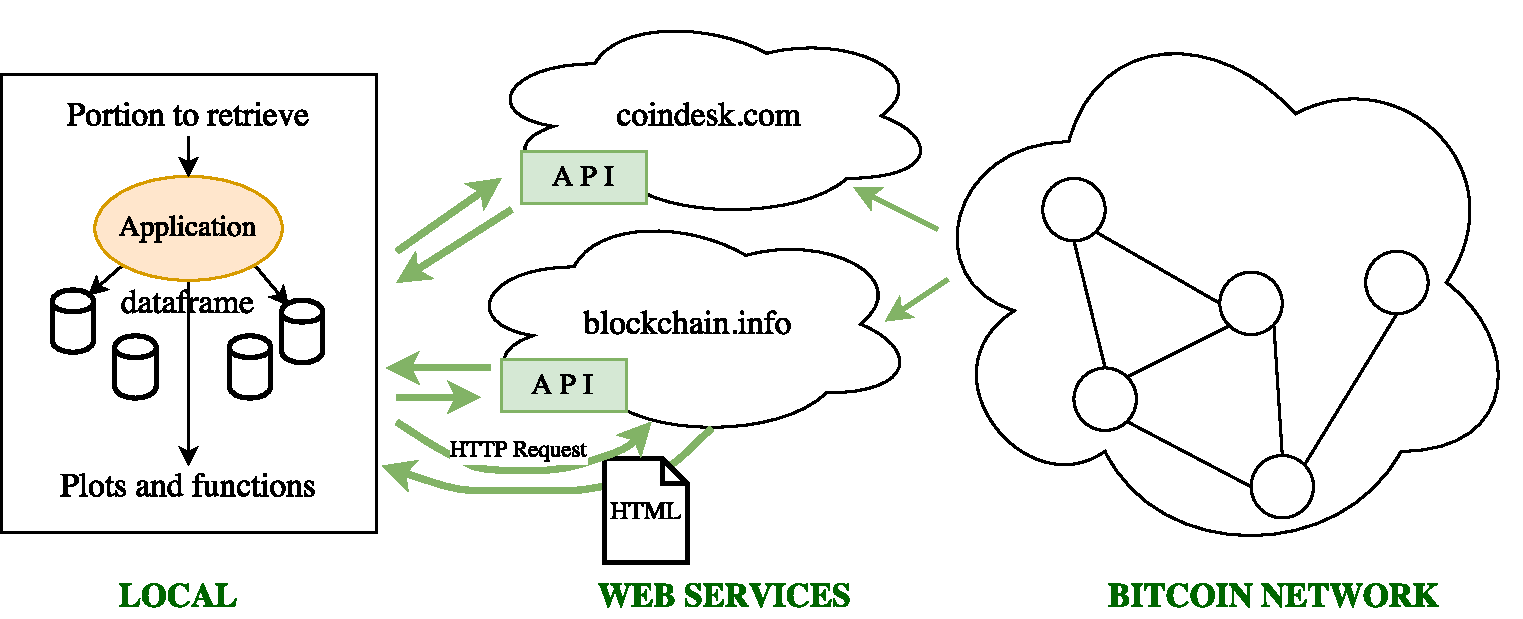
\includegraphics[width=1\textwidth]{img/architecture}
	\caption{Architecture of \gls{bas}.}
	\label{fig:architecture}
\end{figure}

As Figure~\ref{fig:retrieval_scheme} shows,
the information retrieval works
in a combined way, \emph{block-wise}
and \emph{transaction-wise},
information gathered from both sources are
written and stored in $D$. \gls{bas}
collects information from:
\begin{enumerate}[noitemsep]
	\item \textbf{\gls{json}} file sources: files processed block by block and
	for each block transaction by transaction, then information are added to $D$.
	\item \textbf{\gls{html}} file sources: files obtained via a HTTP request. The parsed information are directly added to $D$.
	
\end{enumerate}
\begin{figure}[h]
	\centering
	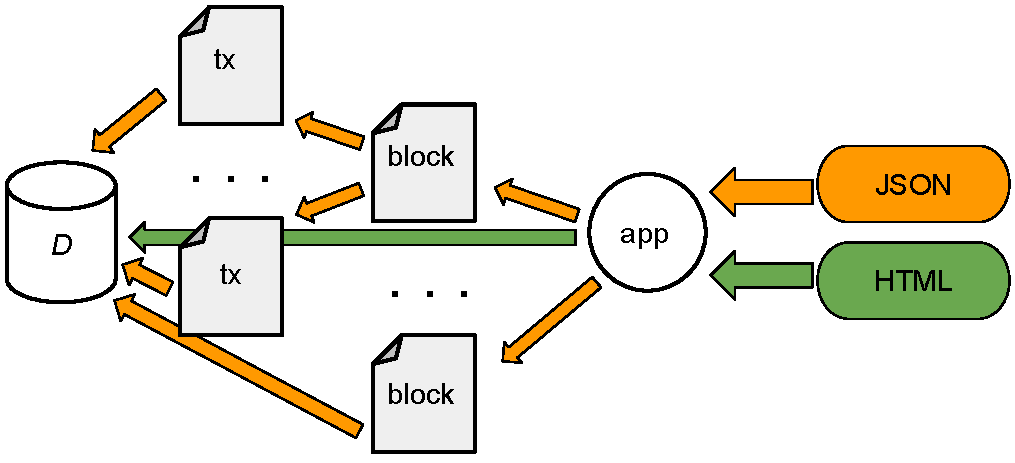
\includegraphics[width=1\textwidth]{img/retrieval_scheme}
	\caption{How information is retrieved and gathered in our data frame $D$.}
	\label{fig:retrieval_scheme}
\end{figure}

\section{Data Sources}
Many websites like \url{tradeblock.com}\,\cite{tradeblock}
or \url{blockchain.info}\,\cite{bitcoin_blockchain}
are observing the Bitcoin blockchain every day.
These websites also provide a remote \gls{api} 
that allows you to retrieve information about
blocks and transactions directly from
the website through \gls{rest} \gls{api}s.
Furthermore, websites like
\url{coinbase.com} provide useful information about the
money exchange price, and they arrange \gls{api} along with
libraries like the one we used, called
\emph{forex-python}\,\cite{forex-python}.
As already mentioned, one of the most
popular system for analyzing Bitcoin
data is Bitcoin Core\,\cite{bitcoincore}.
However, the client requires users to download
the full ledger of data before any analytics
can take place, which at the time of writing was
$125$\,\gls{gb}, with a total disk space required of
$250$\,\gls{gb}.
Since we wanted to optimize and
be able to select data we wished to analyze and
did not have the need to run a full node,
we developed a system for blockchain retrieval and analysis.
This system allows to fetch a portion of the blockchain by
storing data in Pandas data frame\,\cite{pandas}.
This allows saving one order of magnitude of disk space
while still storing all the information
needed for our purpose. Finally, the system
displays all the knowledge acquired,
analyzing data and applying machine learning techniques
on those, using Python libraries
such as \emph{matplotlib}\,\cite{matplotlib} and
\emph{seaborn}\,\cite{michael_waskom_seaborn}.
%Our blockchain analytic system was implemented
%on a MacBook Pro with MacOS Sierra \emph{v$10.12.6$},
%with a $2.8$\,GHz Intel Core i$7$ processor
%and $16$\,\gls{gb}~$1600$\,MHz DDR3 of RAM, using
%JetBrains PyCharm (\emph{v$2017.1.4$}) software as
%text editor and \emph{Python v$2.7.12$}
%as programming language.
Even though we know
Python is not known for its computational speed,
it provides nice access to the
Bitcoin blockchain by using \gls{api}s arranged
by \url{blockchain.info}, allowing the retrieval
of all the information stored in a block and transaction,
plus, its enormous amount of libraries grants
a vast flexibility on which machine learning algorithms
can be applied or which plotting system to use.

\subsection{Data Retrieval}
\label{sec:dataretrieval}
The architecture displayed in Figure~\ref{fig:architecture}
gives information about the different data
gathered in our system.
The system imports Bitcoin \gls{api}s and uses
them for data retrieval. The website \url{blockchain.info}
also provides \gls{rest} \gls{api}s, in that way
requests made to a resource's \gls{uri}
will elicit a response that may be in \gls{xml}, \gls{html}, \gls{json}
or some other defined format. In our case, \gls{rest} \gls{api}s
from Bitcoin return \gls{json} data.
The website \url{blockchain.info} is monitoring
the blockchain $24$-$7$,
producing graphs and
statistical analysis on the
actual Bitcoin network. The local
application is monitoring these data as well,
producing graphs that are not taken into
consideration from this website,
using a finer granularity to represents
the data, allowing us to
do an in-depth analysis on those.
For our analysis we select a time range from April~$2013$ to
September~$2017$, considering more than one hundred
twenty million of transactions
and one hundred thousand of blocks. Before $2013$, analyses
on the system were already performed and
evaluated\,\cite{croman2016, houy2014EOBTF,
	Moser2015, Rizun:2015:blocksizelimit}
plus the popularity of the system before
$2011$ was low and interpreting this early data would
not be useful and might even be self-defeating in order
to understand system's behavior.
\begin{table}
	\centering
		\caption{Data sources and information gathered}
		\label{tab:datasources}
	\begin{tabular}{|p{3cm}p{3cm}p{4cm}|} \hline
			\textbf{Source}&\textbf{Entity}& \textbf{Information}\\
			\hline
			Blockchain.info \gls{api}s&Block, Transaction&$B_{ha}$, $t_{ha}$, $B_t$, $B_h$, $\mathcal{T}$, $Q$, $t_{in}$, $t_{ou}$, $t_q$, $B_{epoch}$, $t_{epoch}$\\
			\hline
			Blockchain.info \gls{html} parsing&Miner& $B_{mi}$\\
			\hline
			Coindesk.com&Price&\gls{usd} and \bitcoinA~value\\
			\hline
			Data frame $D$&Block, Transaction, Miner, Price&$\tau$, $t_f$, $t_l$, $\gamma$, $\rho$, $t_\%$\\
			\hline
		\end{tabular}
\end{table}
To have an overall view of the entire Bitcoin network
we combine data from different sources. As Table~\ref{tab:datasources}
shows, we use both \url{blockchain.info} \gls{api}s and HTTP parsing
to gather information about blocks, transactions and miners,
plus we used \url{coindesk.com}~\gls{api}s\,\cite{coindesk, forex-python}
to gain information about the pricing of \gls{usd} and \bitcoinA.
Unfortunately \gls{api}s from \url{blockchain.info}
do not allow us to
retrieve all the information we need,
knowledge regarding miners is
not included in the blockchain, so we
need to get this information by parsing
web pages on \url{blockchain.info}.
Finally, additional useful information and derived data
such as throughput $\gamma$ or transaction
fee $t_f$ are obtained using our
data structure $D$~(Chapter~\ref{sec:dataorganization}),
containing both, this new
information and the previously collected ones.
An example of data retrieval is shown in Appendix~\ref{lst:jsonretrieval}
and the retrieved block and transaction structures
by using \gls{rest}ful \gls{api}s is
shown in Appendix~\ref{lst:block},\,\ref{lst:transaction}.

%TODO: Shows in the appendix the lst of the retrieval - intervals
\subsubsection{First idea, Blockchain Splitted in Portions}
During our analysis we evaluate different possible ways
to retrieve data. Because of its relevant size
and its fast growth, we considered the blockchain as
an object and we thought that analyzing different
portions over time following a certain pattern would
give us an accurate summary of the whole system. We
started retrieving data by dividing the blockchain in
$k$ portions.
Suppose now that $m$ is the last
block's height, then we divide
all in $k$ portions, having $p = m / k$.
While retrieving $b$ blocks, they are
retrieved and stored in the following way:
\[\langle 1 \dots b\rangle, \langle p \dots p+b\rangle, \langle 2p \dots 2p + b \rangle, \dots , \langle kp \dots kp+b\rangle.\]
Retrieving blocks in such portions gives
statistical representation of the whole system.
Like Figure\,\ref{fig:portions} shows,
every new $b$ blocks added to the
blockchain will be added to the indexes:
\begin{equation}
ip + b\textrm{ }
\begin{cases}
\textrm{for } i = 0 \textrm{ to } k.
\end{cases}
\end{equation}
\begin{figure*}[h]
	\centering
	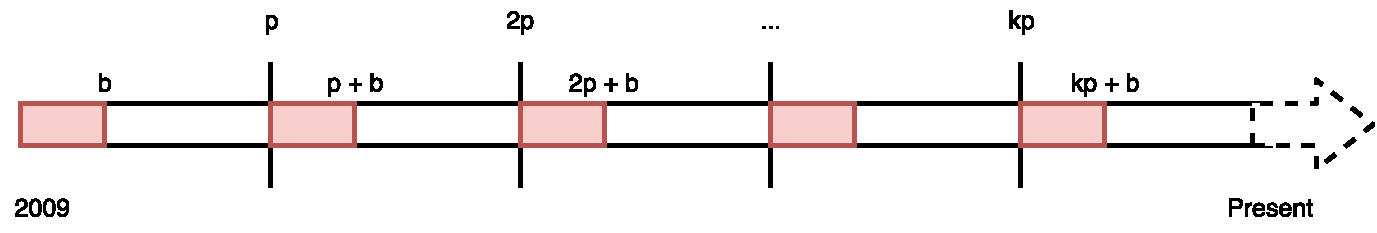
\includegraphics[width=1\textwidth]{img/portions}
	\caption{Science of Bitcoin blockchain, the entire blockchain considered as
		an object and divided in $k$ portions. One of the first attempts of data
	retrieval on Bitcoin blockchain.}
	\label{fig:portions}
\end{figure*}
Retrieving data in this way reduce drastically the space requirements
and yet retaining information about the whole system. However, data
collected using these methods were not enough to achieve
our target of longitudinal study and analysis,
but this technique gave us
a spark for the next data retrieval attempt.

\subsubsection{Fragmented Blockchain}
In the next approach, we use much smaller
interval between each portion
retrieved, called jump or $J$. Plus
we do not retrieve the earliest part of the
blockchain, the one from $2009$ to $2013$.
By retrieving $10$ blocks each time,
according to the granularity of $J$ we can
have a more or less precise analysis. To balance
disk space and precision, we choose a $J = 10$
and a $b = 10$ blocks retrieved each time
we performed \gls{bas}.
This means that every $10$ blocks retrieved, there was
a jump of other $10$ blocks, corresponding to the $\sim$$50\%$
of the entire blockchain, daily analyzed. Figure\,\ref{fig:portions_new}
shows how our last data fetching has been implemented,
so $D$ is generated accordingly, collecting transactions
happened in one hundred minutes and
then having one hundred minutes of gap.
This method allowed us to collect relevant
information from $2013$ to $2017$ by only
using $\sim$$25$\,\gls{gb} of disk space.
\begin{figure*}[h]
	\centering
	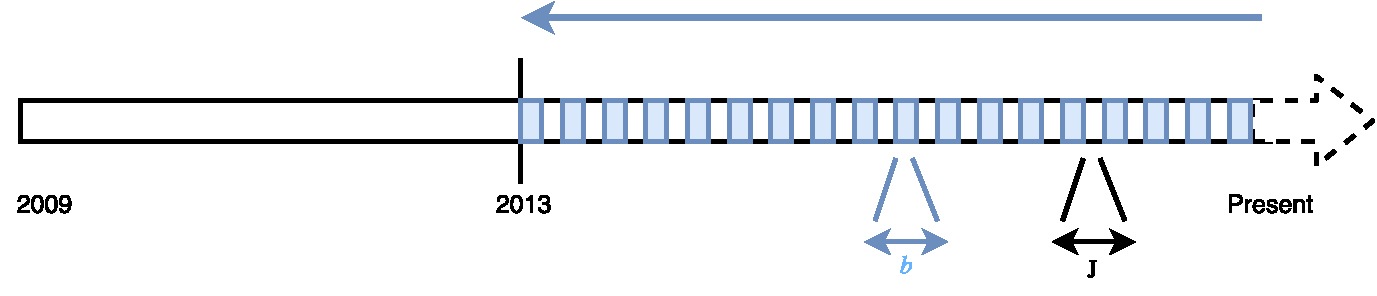
\includegraphics[width=1\textwidth]{img/portions_new}
	\caption{Fragmented blockchain divided in smaller portions with
	a jump of $J$ blocks.}
	\label{fig:portions_new}
\end{figure*}
Then, the pattern we have chosen to store
transactions is the following:
\[\langle m \dots m-b\rangle, \langle m-b-J \dots m-2b - J\rangle, \dots , \langle m-(k-1)b -(k-1)J \dots m - kb - (k-1)J\rangle.\]
And we can write the indexes for each portion that has to be retrieved
according to Equation~\ref{eq:patternfragmented},
following the format $\langle \text{start} \dots \text{end}\rangle$:
\begin{equation}
\label{eq:patternfragmented}
\langle m-ib+b-iJ+J\dots m-ib-iJ+J\rangle
\begin{cases}
\textrm{for } i = 1 \textrm{ to } k.
\end{cases}
\end{equation}

Having $m$ as the height of the most recent retrieved block and $k$ number
of portions. An example of this retrieval method is shown in
Appendix~\ref{lst:portionsretrieval}.

\subsection{Data Organization}
\label{sec:dataorganization}
Figure~\ref{fig:retrieval_scheme} shows how data,
once retrieved, are collected and gathered
in \gls{bas}.
The Pandas package makes it possible
to read data into a specialized data structure
called a \emph{data frame}\,\cite{pandas}.
As argued by Michael Bowles\,\cite{bowles2015machine},
you can think of a data frame as a table or matrix-like
structure with a row representing a single case
or observation and columns representing particular attributes.
We decided to use a data frame structure and not a
matrix because even though the data frame structure
is matrix-like, its elements in various columns may be of
different types. For statistical problems, the matrix is too
confining because statistical samples typically have a mix
of different types, in addition, Pandas package makes it possible
to automate the steps to calculate \emph{mean}, \emph{variance},
\emph{median}, \emph{group-by} elements, and it
offers a nice and smooth control over the data. 

Finally, once data are
retrieved and collected, they are saved in a data frame
structure that we call $D$.
Derived data such as $\gamma$ or $\rho$,
useful for the blockchain analysis, are obtained using $D$.
This data structure is divided among multiple files
with an overall size of $\sim$$25$\,\gls{gb} and it contains
both numerical and categorical variables, saving an average
of $5$ times the amount of disk space compared to the same
information you get by downloading the full ledger,
reaching peaks of $10$ times for some blocks.
In $D$, information is stored in a bi-dimensional table,
with transaction samples represented in
rows and their attributes in columns.
If we consider a set of attributes as a transaction, $T$,
and a set of transactions $D$, then we have
$
T = \{ a_1, a_2, \dots, a_m \}
$
and
$
Y = \{ T_1 \cup T_2 \cup \dots \cup T_n \}.
$
Our data frame $D$ will have then a cardinality of $|D| = (m \times n)$
and it will be structured as shown in Equation~\ref{eq:dataframe}.

Once defining the structure for our dataset $D$,
we consider a set $T$ having the following
attributes (Appendix\,\ref{app:LOS}):
\[
T = \{ t_{ha}, t_{in}, t_{ou}, t_f, t_q, t_\%, t_l, Q, \mathcal{T}, B_h, B_{epoch}, B_t, B_{ha}, B_{mi} \}.
\]
We structure the way our data are stored in order to do
subsequential sampling.
This is the reason why we stored transactions
ordered by block and each block ordered by height/epoch,
in that way we have the dataset ordered by block creation
with all its transactions, making it easier to do analyses
or sampling data in a chronological order.
Summarizing, our data frame allows us to collect all
the useful information without storing the whole raw
blockchain like current systems for
blockchain analysis\,\cite{bitcoincore} do.
Raw data are
collected in \gls{json} format, analyzed, printed to our data frame
and then deleted. This yielded up to save $10$ times the
amount of disk space,
storing in a $1$\,\gls{gb} data frame what the raw files
from \url{blockchain.info} store in $10$\,\gls{gb} space. Plus, we
believe that analyzing a small percentage of the blockchain
everyday will give us relevant information about the
whole system. Due to time limitations we could only collect $50$\%
of the data, every day.

\subsection{Data Visualization}
\label{sec:datavisualization}
%TODO: ============= VISUALIZING DATA ============
Once data are retrieved and saved in our data structure $D$,
is finally possible to get the information we need out of them.
Even though Pandas offers a nice way to plot your data, 
visualizing big data might be not always immediate or intuitive,
and a study on how to plot your data is necessary if you want
to gain the right information out of it.
Once data are ready to be analyzed, the first
step is to determine the outliers.
A spontaneous question that came up in our minds is:
\emph{how to deal with outliers?} We could segregate them
out and train on them as a separate class, or easier, when
data are grouped, a median is calculated instead of the mean,
since mean is extremely sensitive to outliers.
Dealing with categorical attributes instead, as the number
of attributes grows,
the complexity of handling them mounts,
also, most of binary tree algorithms, which are the basis for
ensamble methods, have a cutoff on how many
categories they can manage\,\cite{bowles2015machine}.
Random Forest package written by Breiman and Cutler
has a cutoff of 32 categories\,\cite{Breiman:2001:RF}.
Our only categorical variable is $B_{mi}$ so we
did not deepen the analysis of categorical attributes.

To visualize our data we use Pandas libraries
as well as \emph{matplotlib} and
\emph{seaborn}\,\cite{pandas, matplotlib, michael_waskom_seaborn}.
We mostly use seaborn when we need to plot data
according to a certain category, so we need multiple
samples for each $(x,y)$ point, e.g.
Figures~\ref{fig:trendy_miners},~\ref{fig:fee_latency}.
We use it to
calculate how major mining pools change their
number of transactions approved over time, or to
calculated the $\rho$ for every mining pool. We also
use it to calculate the linear regression and the Pearson's
coefficient for every attribute $a \in D$.
Pandas was used mainly for area plots and pie plots,
e.g. Figure~\ref{fig:txs_fee_distribution},~\ref{fig:txs_feedensity_distribution}.

One example of data manipulation and visualization on our
dataset $D$ regards to the calculation and classification
over time of the fee density, $\rho$. From $D$, we collected
the data we needed and we generated another data frame $D'$.
In that way we have a new data frame with a new set of attributes
$X'$, generated according to to the transformation
we need, calling it for brevity
$\xrightarrow{\text{$\lambda$}}$, having then
\[
D \xrightarrow{\text{$\lambda$}} D',
\]
\[
T \xrightarrow{\text{$\lambda$}} X'.
\]
So the transformation $\xrightarrow{\text{$\lambda$}}$ brings a new set
of attributes with new data in it.
This new $X'$ contains a set of numerical values categorized, 
regarding $\rho$,
plus the related date and the total number of transactions approved in
the following way:
\[
X' = \{\text{0, <50, <100, <200, <300, >300, date, total} \}.
\]

Another use of data manipulation for visualization is the one we apply to
the epoch. We want to make our data more readable and categorize the
time, by transforming
our epoch in date time and then get only the information we need
regarding the day, the month or the year. By doing that we have to
apply a function to our data frame $D$ that hits one attribute
(in this case the epoch, $B_{epoch}$), convert it to date
and then parse it to get information about the day, month or year.
The listing is shown in Appendix~\ref{lst:epochdatetime}.

\subsection{Derived Data}
As shown In Table~\ref{tab:datasources}, our data frame $D$ gives
us information about derived data, from other data
collected. This section aims to explain how they are
calculated and why they are so important. We first focus on
calculating the exact amount a transaction has to pay in order to
get the payment processed and approved: the transaction fee,
$t_f$. This fee is a difference between the sum of all
inputs $t_{in}$ and the sum of every output $t_{ou}$ of a transaction $t$.
In that way, if $n$ is the number of input and $m$ the number of output,
$t_f$ is calculated according to Equation~\ref{eq:txfee} and measured
in \gls{btc} (\bitcoinA).
\begin{equation}
\label{eq:txfee}
t_f = \sum_{i = 1}^{n}t_{in_i} - \sum_{i = 1}^{m} t_{ou_i}.
\end{equation}
Next, we calculate the time it takes for every transaction $t$, to
be approved in the network: transaction latency, $t_l$.
This value is calculated following
Equation~\ref{eq:txlatency} and is the difference between two epochs,
the first is the block creation time in which
a transaction $t$ is included, the second is the transaction
timestamp, so when it was created. $t_l$ it could be measured in
seconds, minutes or hours.
\begin{equation}
\label{eq:txlatency}
t_l = B_{epoch} - t_{epoch}.
\end{equation}
Another relevant derived information using $D$, is the throughput
of the Bitcoin network, or how many transactions it can approve
per second. We measure it according to Equation~\ref{eq:throughput},
we call it $\gamma$ and the unit used is transactions per second ($tx/sec$).
\begin{equation}
\label{eq:throughput}
\gamma = \frac{t_B}{\mathcal{T}}.
\end{equation}

As stated by Rizun\,\cite{Rizun:2015:blocksizelimit},
information regarding fee density might be of a relevant
interest.
This value, that we represent with
$\rho$, could be an important factor for miners
to chose whether to include a transaction or not in their
next block, and indicates how many \gls{btc}(\bitcoinA) per bytes
a transaction $t$ has to offer. Equation~\ref{eq:feedensity}
shows how $\rho$ is calculated.
\begin{equation}
\label{eq:feedensity}
\rho = \frac{t_f}{t_q}.
\end{equation} 

We also calculate and insert in $D$ the fee paid in percentage,
compared it with the total input of a transaction $t$.
This value might be useful when the
Bitcoin price increases or decreases drastically, in a way that we are
able to monitor if the fee is stable, or changes over time.
Then we calculated $t_\%$ as it is shown in
Equation~\ref{eq:tpercentage}:
\begin{equation}
\label{eq:tpercentage}
t_\% = 100 - \frac{f_{ou} \times 100}{f_{in}}.
\end{equation}

The last derived data is the block propagation time, $\tau$.
The calculation
of this value follows the papers from Decker and
Croman\,\cite{Decker2013IPBN, croman2016}. From $2012$
to $2015$ block propagation time had an increment.
When it was tested from Decker and Wattenhofer in
$2012$ the median and $90$-percentile time for Bitcoin
nodes to receive a block was $6.5$ seconds and
$26$ seconds respectively. Considering that
at the time of their measurements, the average block size was $87$\,\gls{kb},
a full $1$\,\gls{mb} block would have taken $5$ minutes to be
visible for $90\%$ of the nodes in the network.
In $2015$, the last measurements from Decker and Croman showed
that the $10\%$, median, and $90\%$ block propagation times were
$0.8$ seconds, $8.7$ seconds, and $79$ seconds respectively.
Further, the average block size was at the time roughly $540$\,\gls{kb}.
Projecting to a $1$\,\gls{mb} block size, the $90\%$, median, and
$10\%$ block propagation times would be $2.4$\,min, $15.7$\,sec,
and $1.5$\,sec respectively. We consider this last measurement
our reference for the block propagation time $\tau$.

%One of the reason why Python is chosen as a programming language is because
%data structures are easy to manage and it offers many libraries such as Pandas or Seaborn for data analysis and visualization.
%
%\section{Version Control}
%\label{sec:versioncontrol}
%For the version control on the source code, a public \emph{git} repository at:
%\url{https://github.com/ted92/blockchain.git} was created. Git version \emph{2.6.4}
%is used in the local environment and every significant update is pushed to the
%repository to keep a history of all the changes and how the application was
%developed.
\begin{table}
	\begin{threeparttable}
		\caption{Possible Relations Between Major Attributes}
		\label{tab:assumptions}
		\centering
		\begin{tabular}{|p{1.4cm}|p{0.8cm}|p{0.8cm}|p{0.8cm}|p{0.8cm}|p{0.8cm}|p{0.8cm}|p{1.1cm}|p{0.8cm}|} \hline
			&\textbf{$Q$}&\textbf{$\mathcal{T}$}&\textbf{$\tau$}&\textbf{$\gamma$}&	\textbf{$t_f$}&\textbf{$\langle C\rangle$}&	\textbf{$\mathbb{P}_{orphan}$} &\textbf{$t_l$} \\
			\hline
			\textbf{$Q\uparrow$}& \cellcolor{gray!25}& &$\uparrow\uparrow$ &$\uparrow$ &$(\downarrow)$ &$\uparrow$ &$\uparrow\uparrow$ &$(\downarrow)$\\
			\hline
			\textbf{$\mathcal{T}\uparrow$}&$(\uparrow)$&\cellcolor{gray!25}&&$\downarrow$
			&&&&$\uparrow$\\
			\hline
			\textbf{$\tau\uparrow$}&$\uparrow\uparrow$&&\cellcolor{gray!25}&$\downarrow$&$(\downarrow)$&$(\uparrow)$&$\uparrow$$\uparrow$ &$\uparrow$\\
			\hline
			\textbf{$\gamma\uparrow$}&$\uparrow$&$\downarrow$&&\cellcolor{gray!25}&$(\downarrow)$&$\uparrow$&$(\uparrow)$& $\downarrow$\\
			\hline
			\textbf{$t_f\downarrow$}&&&$(\uparrow)$&&\cellcolor{gray!25}&$\uparrow$&&
			$\uparrow$\\
			\hline
			\textbf{$\langle C\rangle\downarrow$}&$\downarrow$&&&&$\uparrow$&\cellcolor{gray!25}
			&&$(\downarrow)$\\
			\hline
			\textbf{$\mathbb{P}_{orphan}\downarrow$}&$\downarrow$&&&&&$\downarrow$& \cellcolor{gray!25}&\\
			\hline
		\end{tabular}
		\begin{tablenotes}
			\item[1] $\uparrow\uparrow$/$\downarrow\downarrow$: more than linear or
			even exponential
			increase/decrease
			\item[2] $\uparrow$/$\downarrow$: increase/decrease.
			\item[3] $(\uparrow)$/$(\downarrow)$: might increase/decrease.
			
		\end{tablenotes}
	\end{threeparttable}
\end{table}
\section{Assumptions}
\label{sec:assumptions}
Our focus and studies
are related to blockchain scalability, performance and
to investigate whether the constant
increase of transactions per day
affects the way miners include transactions
or the way users offer fees to miners.
We assume that, analyzing the last $5$\,years
of transactions might produce interesting
results about how this system is evolving and changing its
properties, and how this properties are related
between each others.
We studied and analyzed previous works on the Bitcoin
blockchain\,\cite{croman2016, Rizun:2015:blocksizelimit,
	Moser2015, Decker2013IPBN}
and we made some assumptions of how
the following properties of the Bitcoin systems may vary if other
attributes are changed as well. We tried to classify the main
properties of the system and make assumptions on how they
may vary. These attributes are $Q$, $\mathcal{T}$, $\tau$,
$\gamma$, $t_f$, $\langle C\rangle$, $\mathbb{P}_{orphan}$ and $t_l$ and
our assumptions are summarized in Table~\ref{tab:assumptions}. For
each property, the rows describe what happens to other attributes
if the attribute considered, is increased/decreased. White spaces
means that there might be no relation or we do not have any assumption
yet. For example, if we are going to increase the block space $Q$,
then we have a relevant increase of the propagation time, $\tau$,
the chances of orphaning are way bigger, so it will be the cost of mining a block,
but we have a better throughput $\gamma$, and we might have
less fee from transactions, $t_f$, since they will have less competition
while trying to be included in a block.

\chapter{Observations}
\label{chap:evaluation}
In this chapter we present and discuss observations of the
Bitcoin blockchain, captured by the
analytic system outlined in Chapter~\ref{chap:expsetup}. 
To evaluate and discuss our problem definition in Chapter~\ref{sec:probdefinition},
we focus on considerations related to performance,
scalability, fees and costs.
To answer our questions and focus on
the problems and possible solutions,
a large number of test has been evaluated,
more than one hundred twenty million
transactions over one hundred thousands
blocks were collected, stored
and analyzed, between April~$2013$ and September~$2017$.
Graphs and relations between attributes are represented
and discussed, and they mine to
verify our assumptions in Table~\ref{tab:assumptions}.
We can finally state that
scalability brought to a centralization problem concerning miners,
since nowadays there are less individual miners and more mining pools,
an unlikely and ill-judged increment of $\mathcal{T}$
that might lead to an excessive high throughput $\gamma$,
and an urgent problem whether to increase the block size $Q$ or not,
due to the massive scale of transactions to approve;
performance studies brought to consider carefully
an increment of $\gamma$ since it may
leads either to a raise in costs $\langle C \rangle$
or a growth of $\mathbb{P}_{orphan}$, while a user-side
performance study concerning the transaction latency $t_l$,
enhanced after $2015$, $t_l$ became strictly
dependent of $t_f$; and finally a study on
tips and tolls brought us to analyze miner's profits
and users' benefits, and thanks to our data collected
we were able to infer the miner profit function
$f_{\langle \Pi \rangle}^2$, which establishes a relation
between a block creation time and a miner's profit
$\langle \Pi \rangle$, and to analyze how the
fee paid to the miner changed over time, studying
also the fee density $\rho$.

%TODO: put the following also in the abstract and in the introduction
%TODO: we show that ... events happening on the bitcoin blockchain might influence fee, tolls and the way blocks choose transactions

%TODO: Our observations could be miners oriented or epoch oriented. Analyzing categorical data such as mining pools we could determine which ones are more effective than others and why a block should most likely be mined by a certain mining pool rather than another. Studying the epoch instead, gave us useful information about the changes and the development of the blockchain during time.

%TODO: In our studies, we focused on finding any correlation between attributes using heat map with \emph{seaborn}\,\cite{michael_waskom_seaborn}. If the heat map chart shows any possible correlation then we study the degree of correlation between two attributes, $corr(u,v)$, which can be quantified using Pearson's correlation coefficient showed in Eq.\,\ref{eq:pearson}. However, calculating the correlations and printing them or drawing cross-plots works fine for few correlations, but it is difficult to get a grasp of a large table of numbers, and it is difficult to squeeze all the cross plots onto a page if the problem has a large number of attributes. For that reason we use a heat map with Pearson's correlation coefficient for pairs of attributes arranged into a matrix where the $m_{ij}$ entry is the correlation between the $i^{th}$ attribute and the $j^{th}$ attribute.

%TODO: The next step wants to get some ideas about the relationship among the attributes and between attributes and labels including also categorical attributes.

%TODO: We used for prediction both, \emph{linear} and \emph{nonlinear} algorithms and we considered that linear models are preferable when the data set has more columns than rows or when the underlying problem is simple, nonlinear models are preferable for complex problems with many more rows than columns of data.

%TODO: To get values in $(0,1)$ the logit function in Eq.\,\ref{eq:logit} is applied to our data.


%TODO: The Bitcoin price has been affected of a high volatility. For that reason, predicting the fee in \gls{usd} that a client might pay is difficult and it might change from the Bitcoin price. According to \emph{Coindesk.com}.... show the bitcoin price!

%TODO: In our longitudinal plot each data point visualizes aggregated data of \# blocks.

%TODO: Talk about the observations during time, how the scalability of the system from # transactions per day to # transactions per day influenced the fees and tolls in the system.
\section{Scalability}
\label{sec:scalability}
Scalability may concern the number
of nodes in the network but also
the amount of transactions requested
per second that the system faces.
The constant growth of
cryptocurrencies popularity rise
many concerns regarding the scalability
of the system. The reward for miners
resulted in an increasing interest in mining, and
the number of nodes for this purpose highly increased
during years.
From that, \emph{mining pools} emerged to solve
the puzzles faster and share the earned reward afterwards.
This creates a centralization problem though, only bigger
mining pools nowadays, such as \emph{AntPool}\,\cite{antpool},
\emph{F2Pool}\,\cite{f2pool},
\emph{BTCC Pool}\,\cite{btcc} or \emph{BitFury}\,\cite{bitfury},
will find a solution to mine new blocks, discouraging a lot of small miners
to join the network.

More scalability problems are related to the growing amount
of transactions that need to be approved every day.
With an average $t_q$ of $500$\,bytes, a fixed estimated
$\mathcal{T}=10$ minutes
and a maximum block size $Q$ fixed at $1$\,\gls{mb}, the outside number
of transactions the system can approve
per second is roughly $3$-$4$ transactions per second.
Compared to systems like VISA that can
easily approve two thousand transactions per second, Bitcoin
or any other digital cryptocurrency using the blockchain
protocol are still far in taking over digital systems such as VISA or
Master Card. However we want to analyze these boundaries and understand
what it possible to do with regards to improving scalability.
%TODO: block size limit, block creation time and transaction size.
%TODO: Transactions increment, Blocks need more space

\subsection{Miners \& Mining Pools}
\label{sec:minersminingpools}
In our data frame $D$, all the information
regarding every single transaction are stored,
including which miner approved it. We analyzed and
tracked down every active miner in the system from $2013$ to $2017$.
With $50\%$ of the total information we evaluate a total number
of $6137$ miners, of which $6066$ are just
occasional nodes not belonging
to any mining pool. Note that this number is
approximate to the number of active miners, and
it counts every mining pool as one, since mining
pools withheld information about miners in their
systems.
\begin{figure}[h]
	\centering
	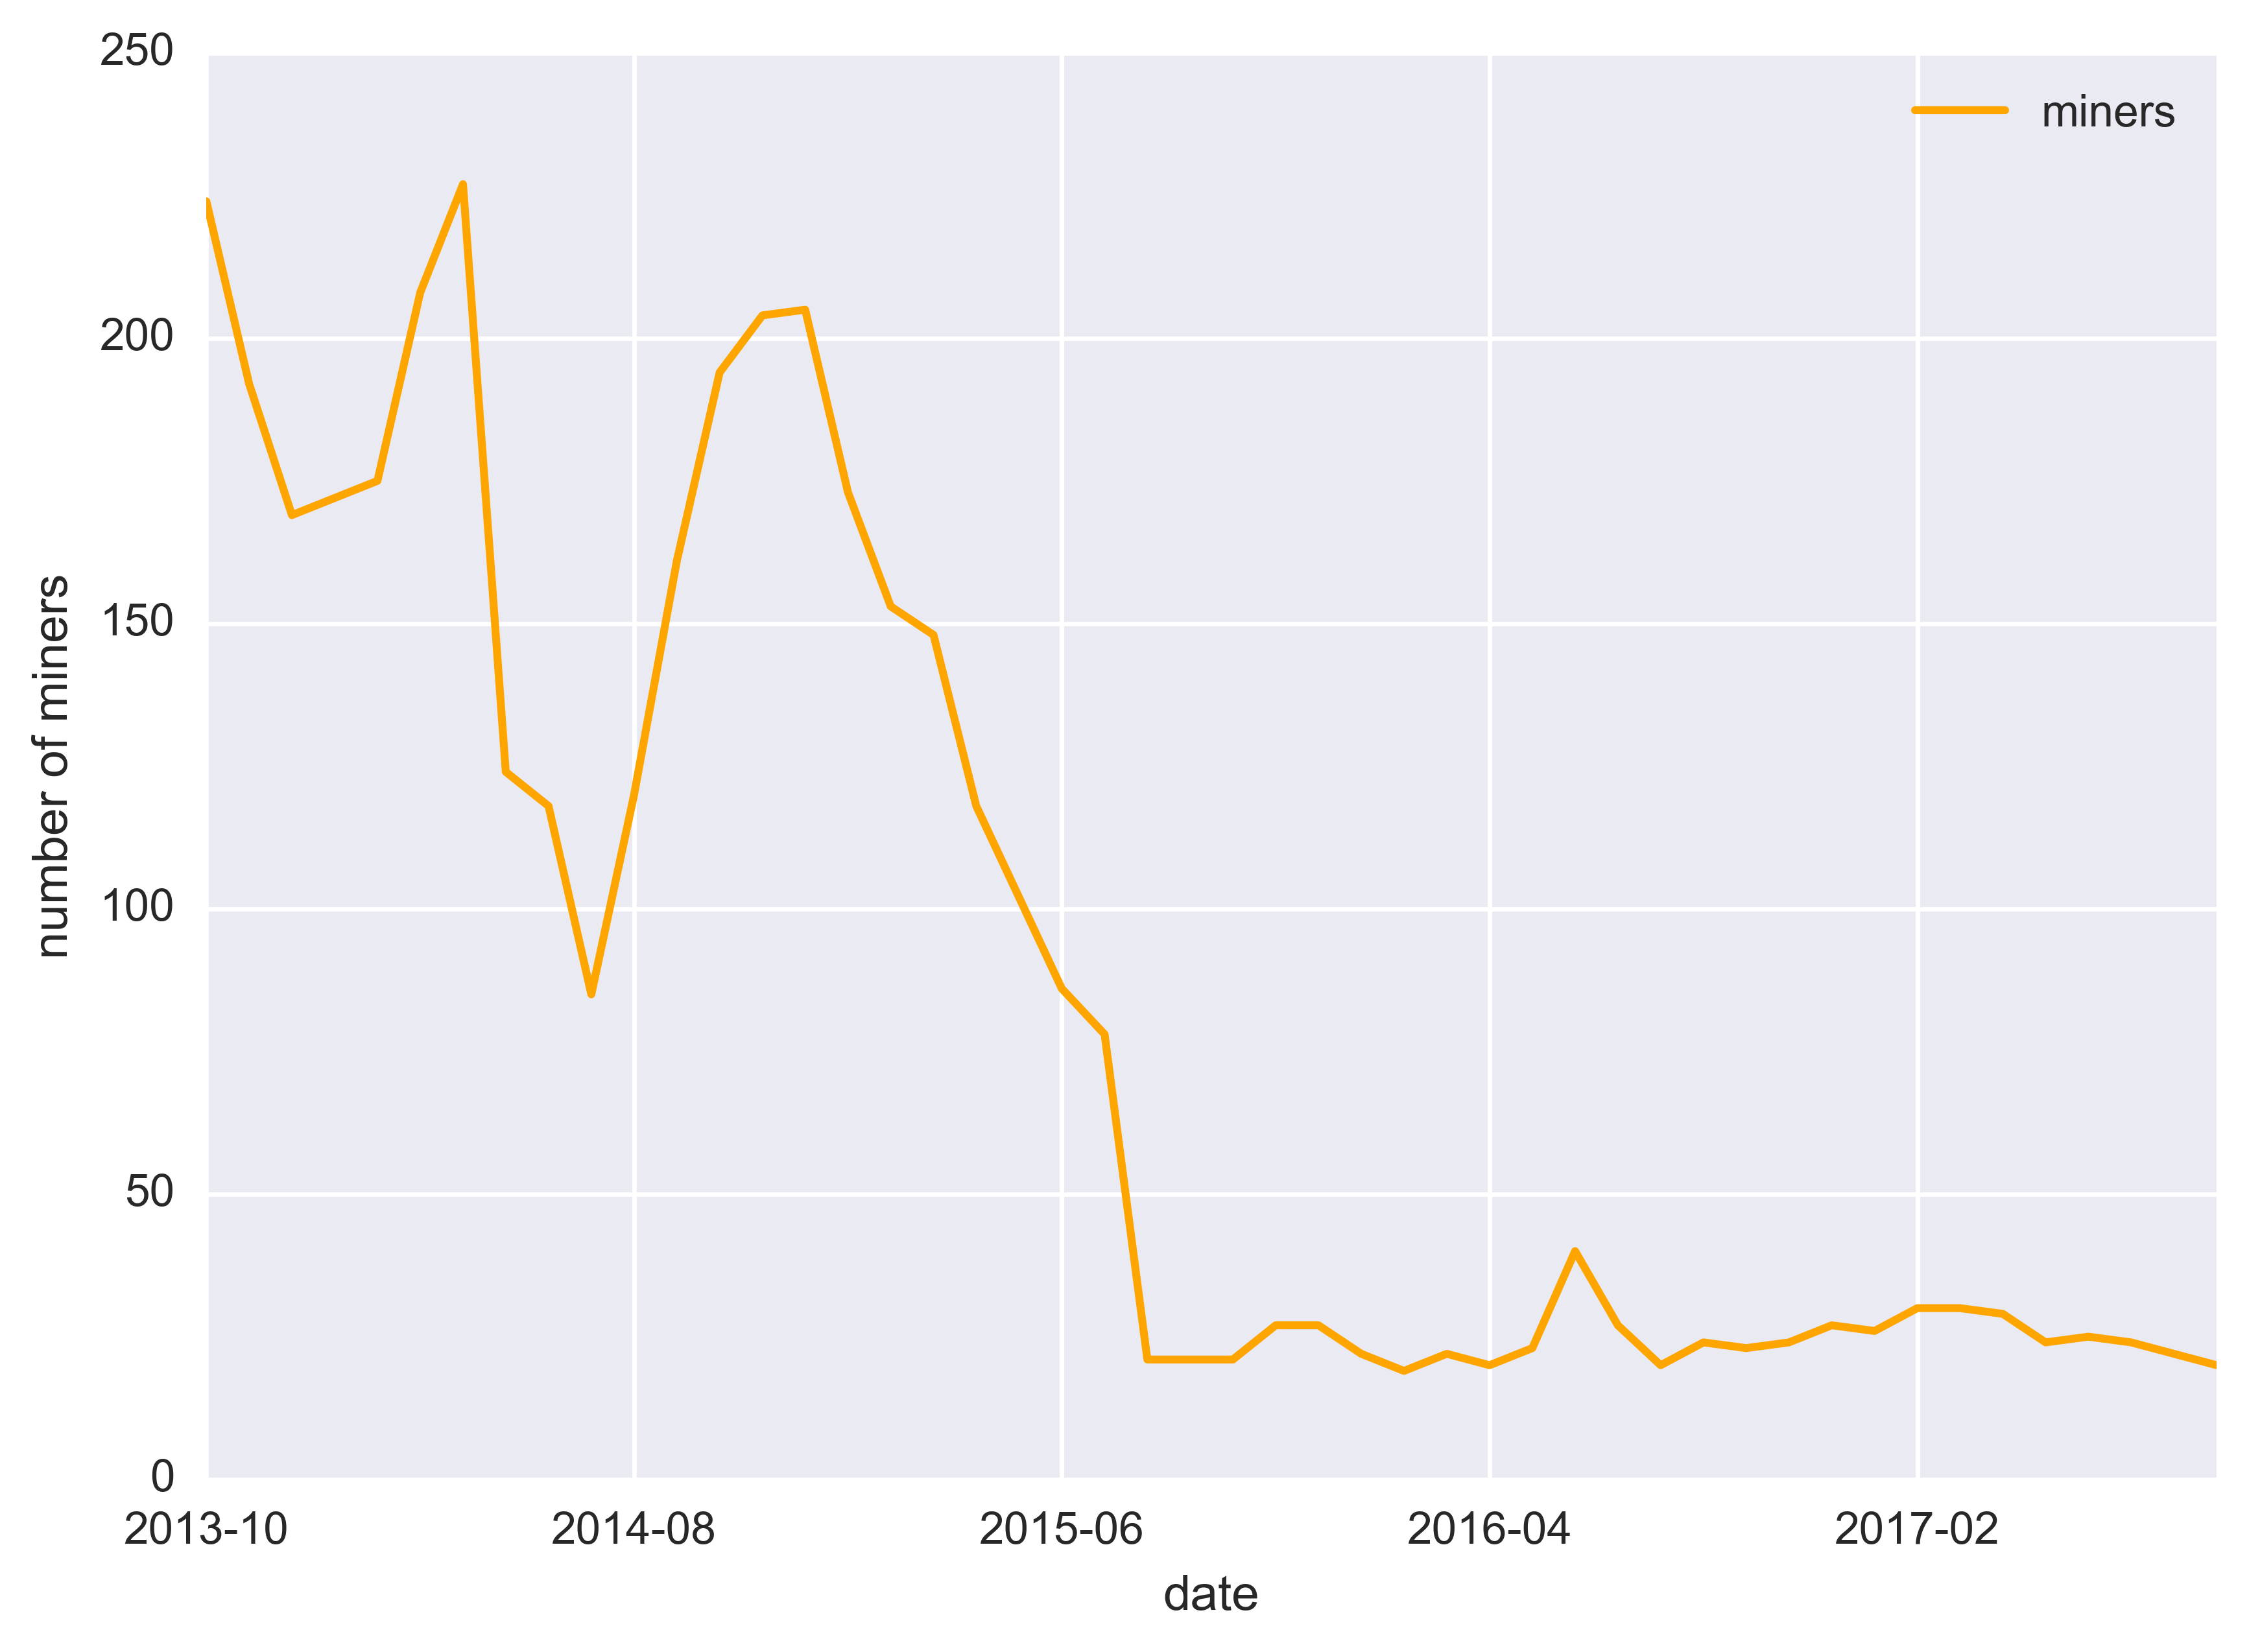
\includegraphics[width=1\textwidth]{img/number_of_miners}
	\caption{Monthly number of active miners from $2013$ to $2017$.}
	\label{fig:number_of_miners}
\end{figure}
In Figure~\ref{fig:number_of_miners} the number
of monthly active miners from $2013$ until now is displayed.
Even if the number is relative to $50\%$ of the
blockchain, we analyze every block mined over time and we state
that after December~$2014$ until August~$2015$
there was a relevant drop, connected to the growth
showed in Figure~\ref{fig:trendy_miners},
mainly caused by the come of mining
pools, KnCMiner, AntPool and BitFury in late $2014$, and the massive
mining power growth of SlushPool and F2Pool in mid $2015$.
This is the main cause of the occasional miners' drop in the system,
and more mining pools will join the network, more it will be
disheartening for smaller nodes to start mining, since the costs
will be probably higher than the revenue.
This creates a sort of centralization problem, since
only the biggest mining pools could take part in the whole
process of approving transactions, forcing small and
occasional miners to join big mining pools.
From our analysis, we state that there are different mining pools
joining and leaving the Bitcoin network during these years.
\begin{figure}[h]
	\centering
	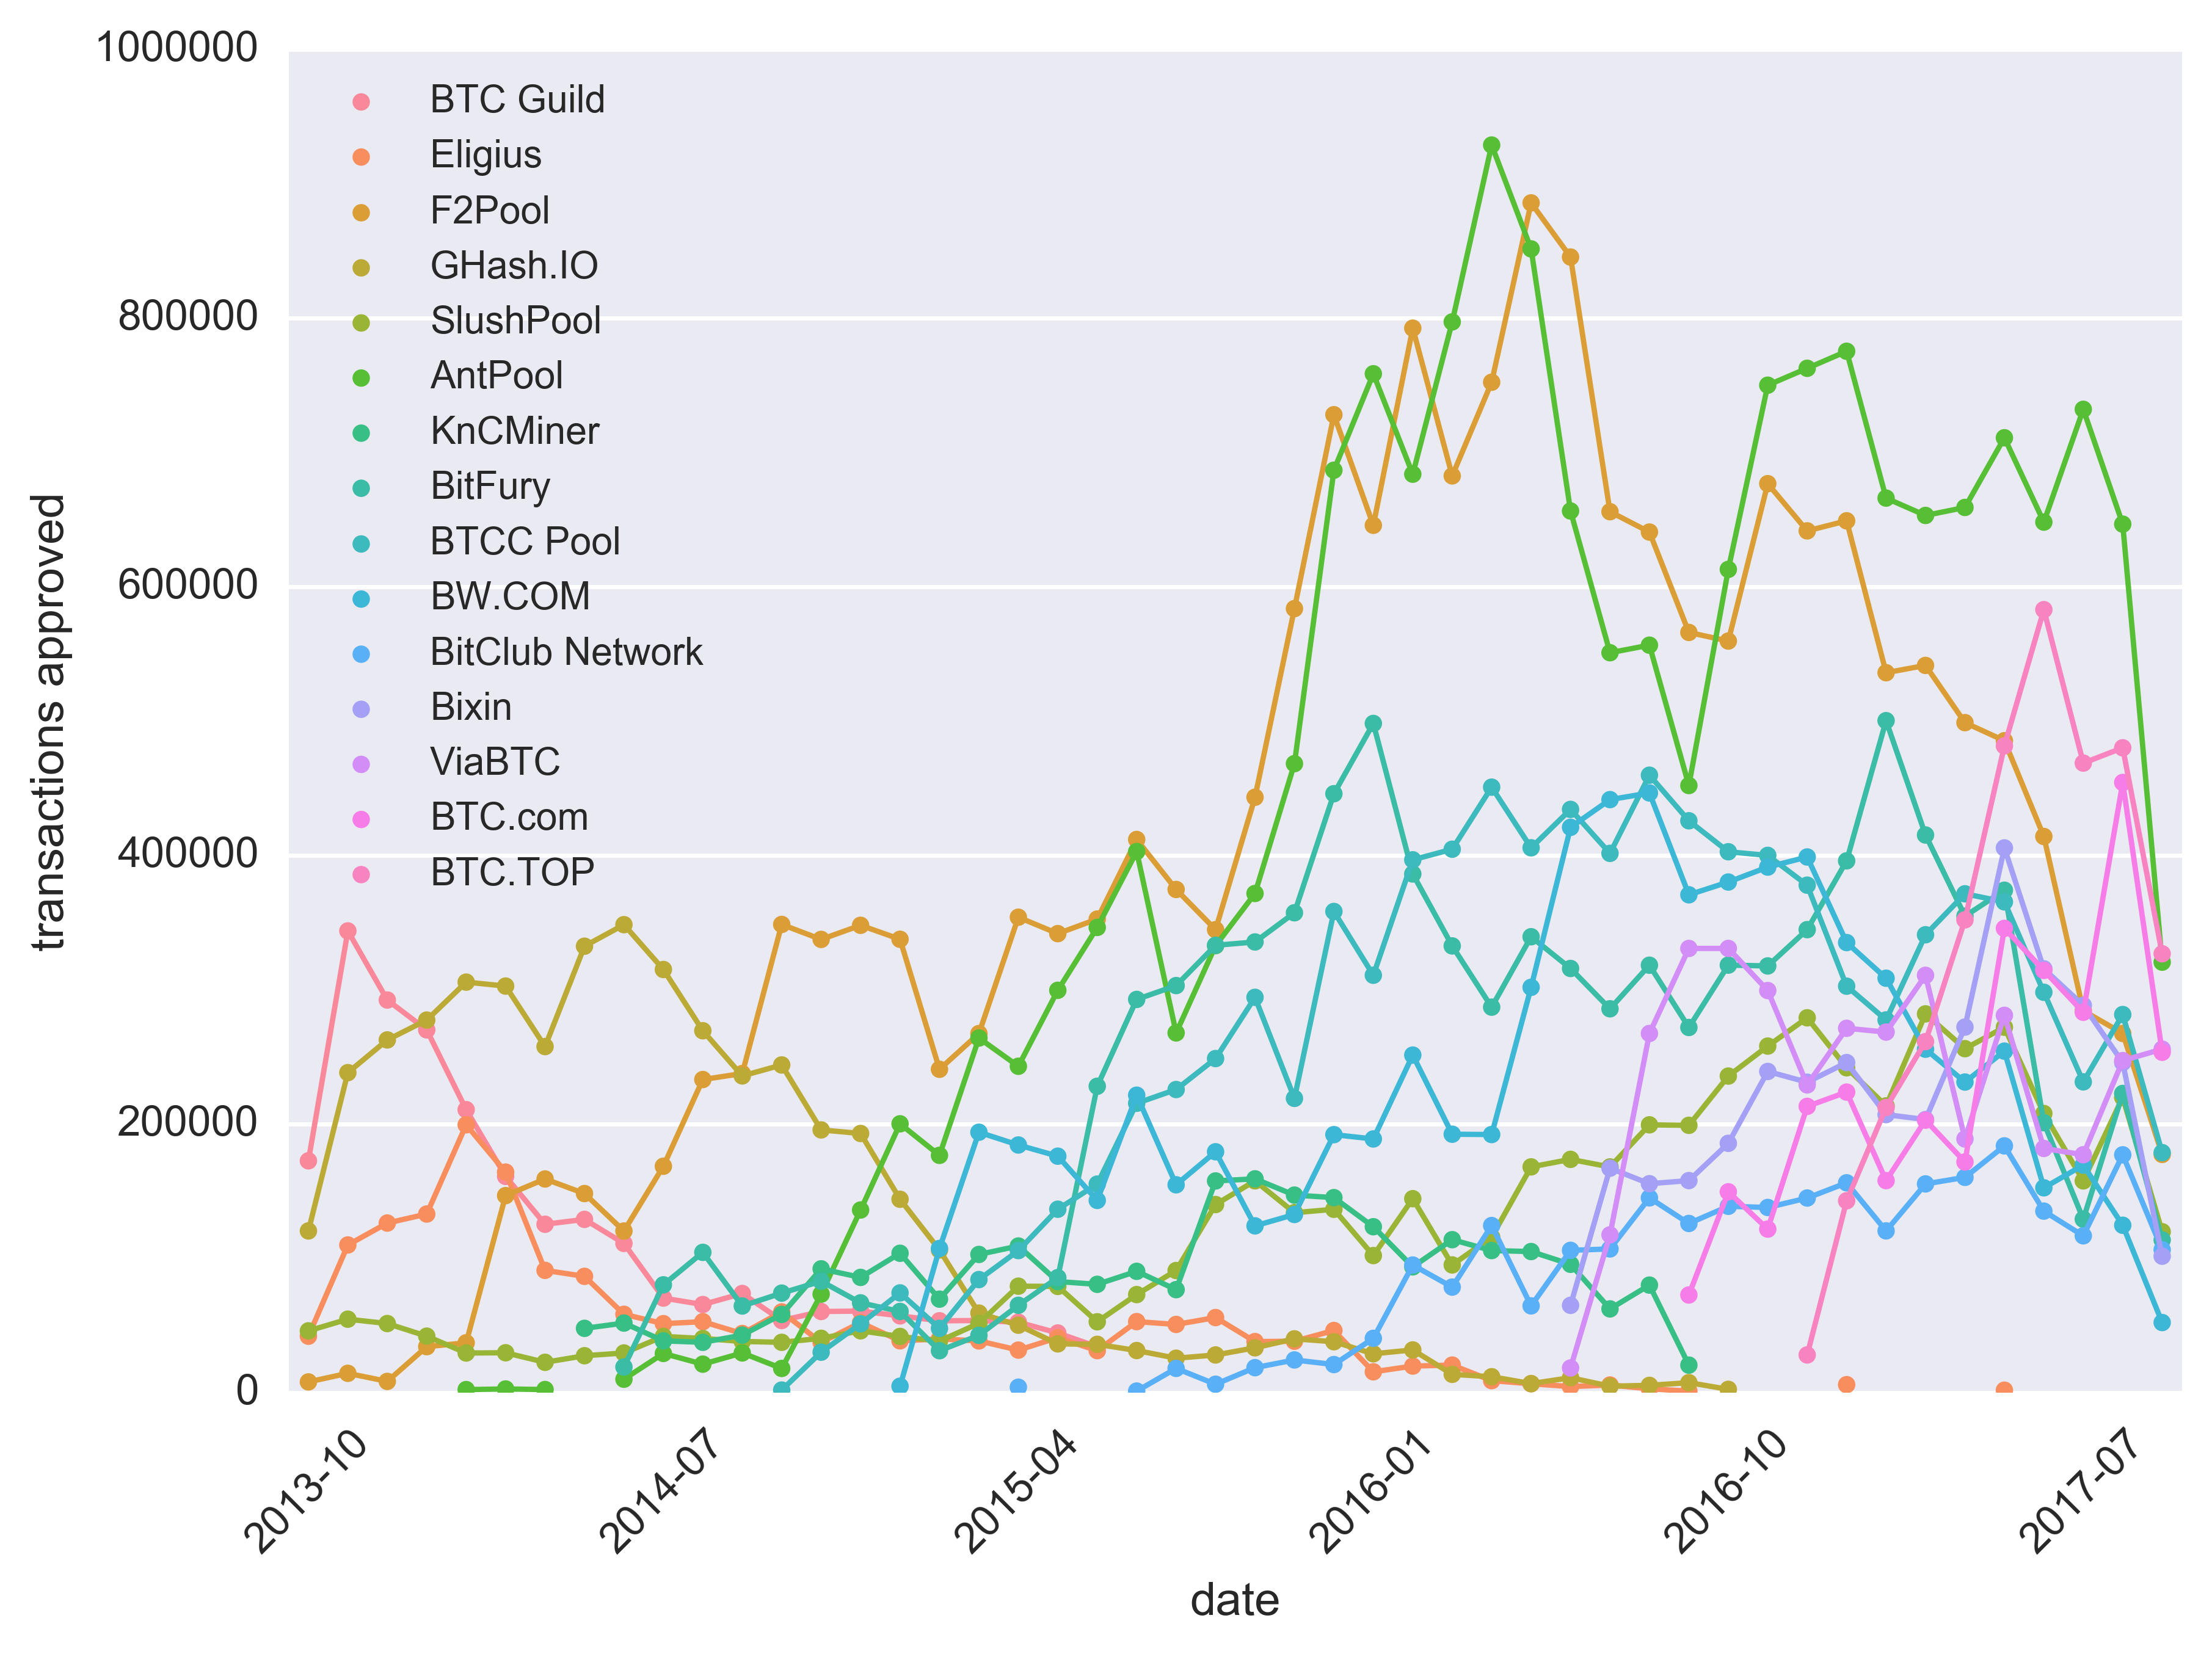
\includegraphics[width=1\linewidth]{img/trendy_miners}
	\caption{Top $15$ mining pools from $2013$ until $2017$ and their trend
		according to the number of transaction they approve every month.}
	\label{fig:trendy_miners}
\end{figure}
\begin{figure}[h]
	\centering
	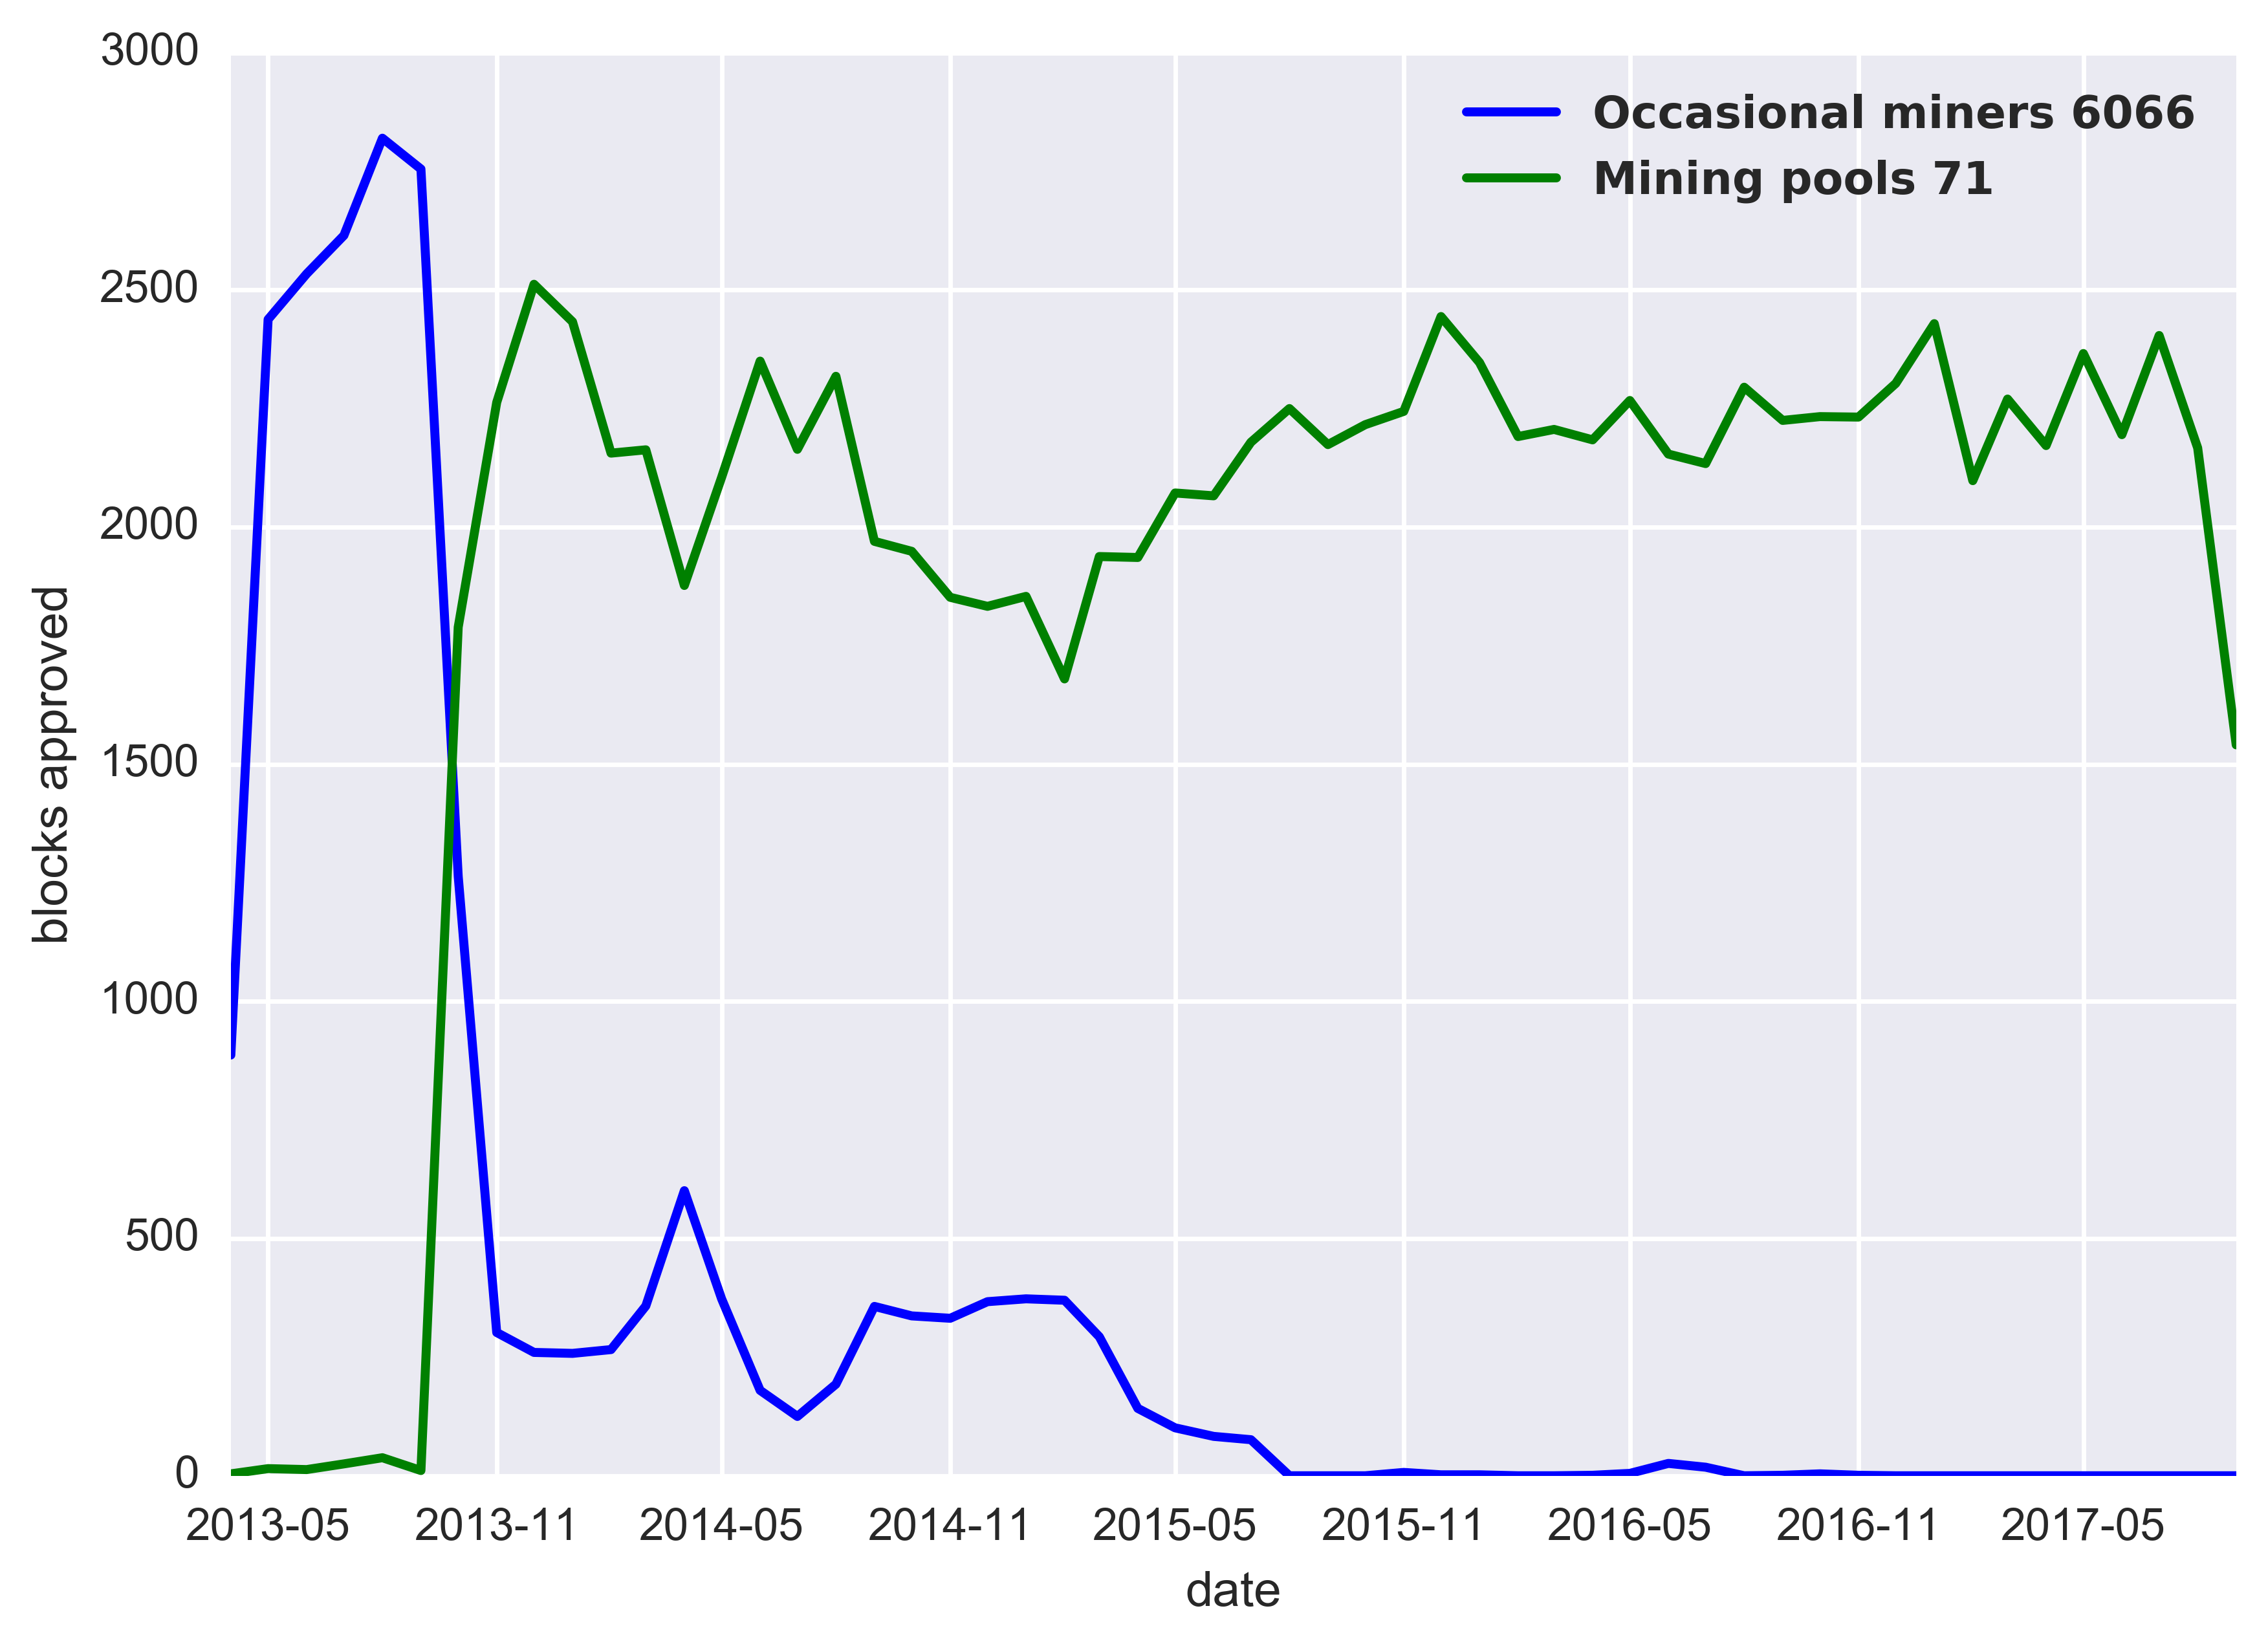
\includegraphics[width=1\textwidth]{img/top_miners_monthly}
	\caption{Number of transactions approved from occasional miners and mining pools from $2013$ until $2017$.}
	\label{fig:top_miners_monthly}
\end{figure}
As Figure~\ref{fig:trendy_miners} shows,
the most relevant example is the \emph{GHash.IO}
pool, which was one of the major mining
pool until mid~$2015$, then its mining power started to decrease
slowly until its end in October~$2016$. We refer to an article
from \url{coindesk.com}\,\cite{coindesk_ghash_ditched}
which says that Bitcoin miners ditched GHash.IO pool over
fears of $51\%$ attack~(Appendix~\ref{app:otherdefinitions}).
Indeed in $2014$, according to \url{blockchain.info},
GHash.IO accounted for more than $42\%$ of Bitcoin mining power.
Nowadays as the Table~\ref{tab:miner_share_2017}
shows, AntPool has $19.53\%$ of
the mining power, and there is no centralization risk.
After that, we analyzed the major mining pools from $2013$ until $2017$,
dividing the time period in two portions,
$2013$-$2015$ and $2016$-$2017$,
and selecting the first $10$ miners regarding their mining power,
as represented in Tables~\ref{tab:miner_share_2015}-\ref{tab:miner_share_2017}.
Table~\ref{tab:miner_share_2015}, shows that a big percentage of the mining
power comes from occasional miners, and for the whole period
between $2013$ and $2015$ GHash.IO only had $13.3\%$ of
share. We can see in Figure~\ref{fig:trendy_miners}
that this mining pool only had a short time peak between $2013$-$2015$,
but anyway in an overall scheme it managed to collect $13.3\%$
of the whole share. Table~\ref{tab:miner_share_2017} shows that
AntPool, F2Pool and BTCC Pool are dominating the mining
power in the Bitcoin network from $2016$ until now with values
respectively of $19.53\%$, $16.43\%$ and $10.5\%$ of share.
If compared with Table~\ref{tab:miner_share_2015}, AntPool
is the one which is growing the fastest, and mining
pools such as GHash.IO and BTC Guild stopped their activity.
We state that today, no miner seems to get
even close to the GHash.IO share in $2014$ and it
seems like we will not have
a centralization problem in the very near future.
However, the mining power over the years
changed from a distributed architecture to a decentralized one.
We can see in Figure~\ref{fig:top_miners_monthly} that
occasional miners almost disappeared in the last two years,
leaving space to mining pools in their absence,
while they were contributing
for almost the $100\%$ at the end of $2013$. This brought a
downside for individual users that want to buy
their own hardware and start mining for themselves.
Since Bitcoin always claimed its distribution as a 
system strength, this scalability issue
might result a centralization problem in the long run,
excluding small miners from the system and letting
only the biggest mining pools to have information
about the whole blockchain. Bitcoin is useful only if is decentralized because
centralization requires trust and Bitcoin value proposition is trustlessness.
\begin{table}
	\centering
	\caption{Mining power distribution in a scenario from $2016$ until $2017$,
		considering the $10$ major mining pools.}
	\label{tab:miner_share_2017}
	\begin{tabular}{|p{3.3cm}|p{3.3cm}|p{3.3cm}|} \hline
		\textbf{Mining Pool}&\textbf{Mining Power (\%)}& \textbf{Blocks Mined}\\
		\hline
		\rowcolor{AntPool}
		AntPool&$19.53$&$9,078$\\
		\hline
		\rowcolor{F2Pool}
		F2Pool&$16.43$&$7,635$\\
		\hline
		\rowcolor{BTCC Pool}
		BTCC Pool&$10.5$&$4,874$\\
		\hline
		\rowcolor{BitFury}
		BitFury&$8.71$&$4,050$\\
		\hline
		\rowcolor{BW.COM}
		BW.COM&$8$&$3,717$\\
		\hline
		\rowcolor{SlushPool}
		SlushPool&$5.26$&$2,447$\\
		\hline
		ViaBTC&$4.8$&$2,222$\\
		\hline
		Bixin&$4.12$&$1,947$\\
		\hline
		BTC.TOP&$4$&$1,857$\\
		\hline
		BTC.com&$3.55$&$1,648$\\
		\hline
		\rowcolor{TablesColor}
		\textbf{Total Analyzed}&$84.9$&$39,475$\\
		\hline
		\textbf{Other Miners}&$15.1$&$6,996$\\
		\hline
	\end{tabular}
\end{table}
\begin{table}
	\centering
	\caption{Mining power distribution in a scenario from $2013$ until $2015$,
		considering the $10$ major mining pools.}
	\label{tab:miner_share_2015}
	\begin{tabular}{|p{3.3cm}|p{3.3cm}|p{3.3cm}|} \hline
		\textbf{Mining Pool}&\textbf{Mining Power (\%)}& \textbf{Blocks Mined}\\
		\hline
		\rowcolor{F2Pool}
		F2Pool&$13.53$&$10,548$\\
		\hline
		GHash.IO&$13.3$&$10,370$\\
		\hline
		BTC Guild&$7.37$&$5,749$\\
		\hline
		\rowcolor{AntPool}
		AntPool&$6.82$&$5,323$\\
		\hline
		Eligius&$4.99$&$3,889$\\
		\hline
		\rowcolor{BitFury}
		BitFury&$4.73$&$3,693$\\
		\hline
		\rowcolor{BTCC Pool}
		BTCC Pool&$3.9$&$3,042$\\
		\hline
		\rowcolor{SlushPool}
		SlushPool&$3.37$&$2,627$\\
		\hline
		KNCMiner&$3.12$&$2,432$\\
		\hline
		\rowcolor{BW.COM}
		BW.COM&$2.67$&$2,064$\\
		\hline
		\rowcolor{TablesColor}
		\textbf{Total Analyzed}&$63.8$&$49,737$\\
		\hline
		\textbf{Other Miners}&$36.2$&$28,225$\\
		\hline
	\end{tabular}
\end{table}

\subsection{Unconfirmed Transactions}
\label{sec:unconfirmedtxs}
Another relevant concern about scalability in blockchains,
is the number of transaction requests the system
can accept. As we state in Chapter~\ref{sec:throughput},
throughput ($\gamma$) may vary according to $Q$,
$\mathcal{T}$ and $t_q$.
The difficulty of the Bitcoin proof-of-work
is adjusted according to the hashing power of the entire
Bitcoin network so that the average time to mine a block, $\mathcal{T}$,
will always be around a certain value. In our analysis, we prove
that $\mathcal{T}$ stays stable for the whole time and this
value is set at $10$\,minutes. In this interval of time, since
the block size $Q$ is set to a limit of $1$\,\gls{mb}, the system can
approximately approve, if we consider an average $t_q$
of $500$\,bytes, $3.3$ transactions per second. This value is calculated
considering the maximum possible block size of $1$\,\gls{mb}.
If we consider the time between $2013$ and
$2017$, the number of daily transactions that need to be approved
scaled from fifty thousand in $2013$ to three hundred thousand
in $2017$, and all blocks are filled over their maximum
capacity since April~$2016$, as Figure~\ref{fig:block_size} shows.
\begin{figure}[h]
	\centering
	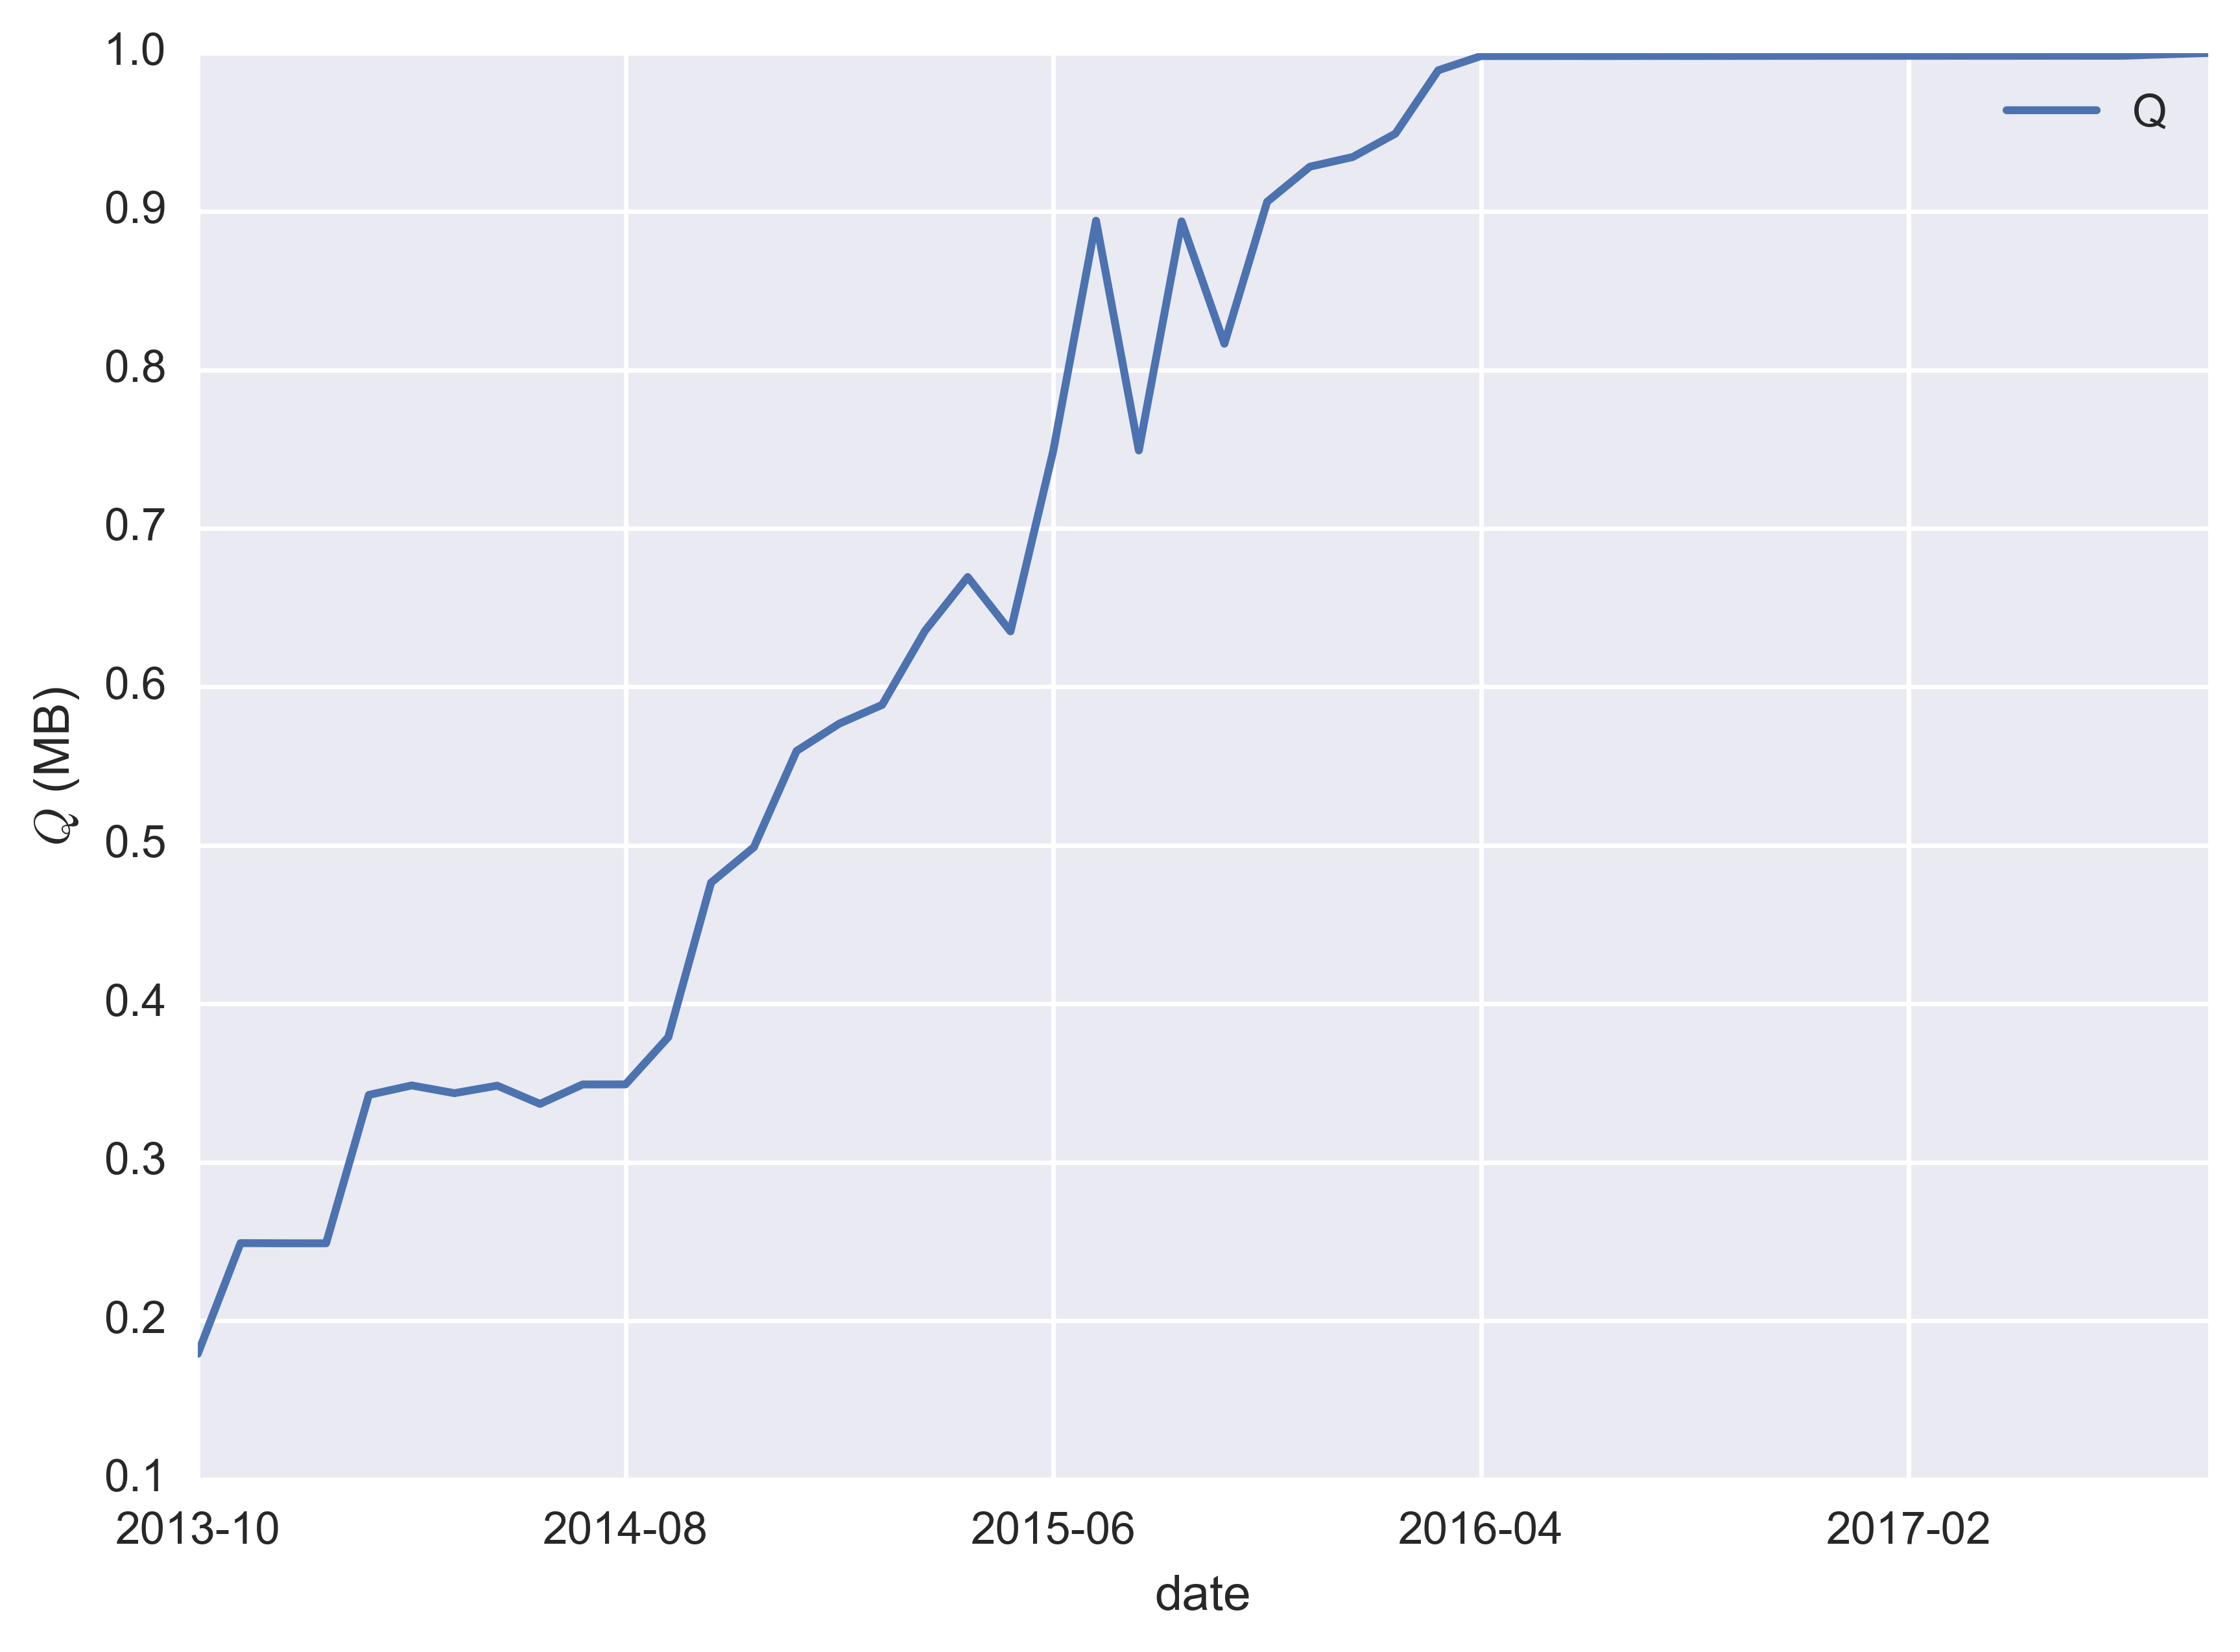
\includegraphics[width=1\textwidth]{img/block_size}
	\caption{Average block size every month, from $2013$ until $2017$.}
	\label{fig:block_size}
\end{figure}
Because of this scaling limitation, transactions might be willing
to pay more fee in order to get accepted in miner's mempools.
To improve the number of transactions that can be
accepted per second by the system, we consider
an eventual change of $\mathcal{T}$ and $Q$, since
we analyzed that the average $t_q$ is constant and equal to
$500$\,bytes for the whole period of testing.

\subsubsection{Block Creation Time $\mathcal{T}$}
In our assumptions, listed in Table~\ref{tab:assumptions}, we argue
that an increment of $\mathcal{T}$ may lead to a
drop in $\gamma$ and an increment on $t_l$, for that reason we believe
that it is a better choice to adjust the difficulty of the proof-of-work in order to
have a shorter block creation time rather than increasing it. Furthermore,
according to Equation~\ref{eq:hashingcost},
the cost of mining a block is directly proportional to the block creation
time, which means that if the $\mathcal{T}$ is decreased, the cost of
mining a block is less. Thanks to our data frame $D$, we managed to
prove that there is an inverse proportionality between $\gamma$ and
$\mathcal{T}$. Only in blocks with a creation time lower than $10$\,minutes,
the throughput reaches peaks of $10$-$14$ transactions per second, while in
cases from $10$ to $20$\,minutes of creation
time, the throughput is between
$2$-$4$ transactions per second and in blocks where the $\mathcal{T}$ is
higher than $20$\,minutes, throughput never reaches
$2$ transactions per second.

Our assumptions about transaction latencies were partially right.
It is true that $t_l$ tends to grow along with
$\mathcal{T}$, but this is true
only if $\mathcal{T} \geq 10$\,minutes. If the block is mined
before that time then we do not have any relation between
transaction latency and block creation time.
We suspected that this uncertain relation might be
somehow connected with who mined that particular block.
While mining pools may have different criteria (higher transaction
fee) while appending transactions to be mined,
occasional miners might have none, or less. This is the reason why
the $t_l$ is so random if $t$ is mined by an occasional miner,
since transactions are not selected
according to any criteria, so a transaction $t$ that did not offer any fee
and has been waiting to be approved for long time, might be included
by some occasional miner if it luckily wins the proof-of-work before
the $10$\,minutes time. After some tests, we show the results in
Figure~\ref{fig:creation_time_miners}. As suspected, for $0 \leq \mathcal{T} \leq 7$,
the occasional miners take the $21.3\%$ of mining share, while in the
other portions they never reach the $18\%$ of the total blocks mined.

In conclusion, an increment of $\mathcal{T}$ is ill-judged, while
decrementing it should be considered, acknowledging, according to
Equation~\ref{eq:orphaning}, that an increased bandwidth
for a better inner node communication is needed, otherwise we
might have an exponential growth on $\mathbb{P}_{orphan}$.
Furthermore, in Chapter~\ref{sec:minersprofit}, we state that
with a higher $\mathcal{T}$ the profit $\langle \Pi \rangle$ of
a miner is significantly lower.
\begin{figure}[h]
	\centering
	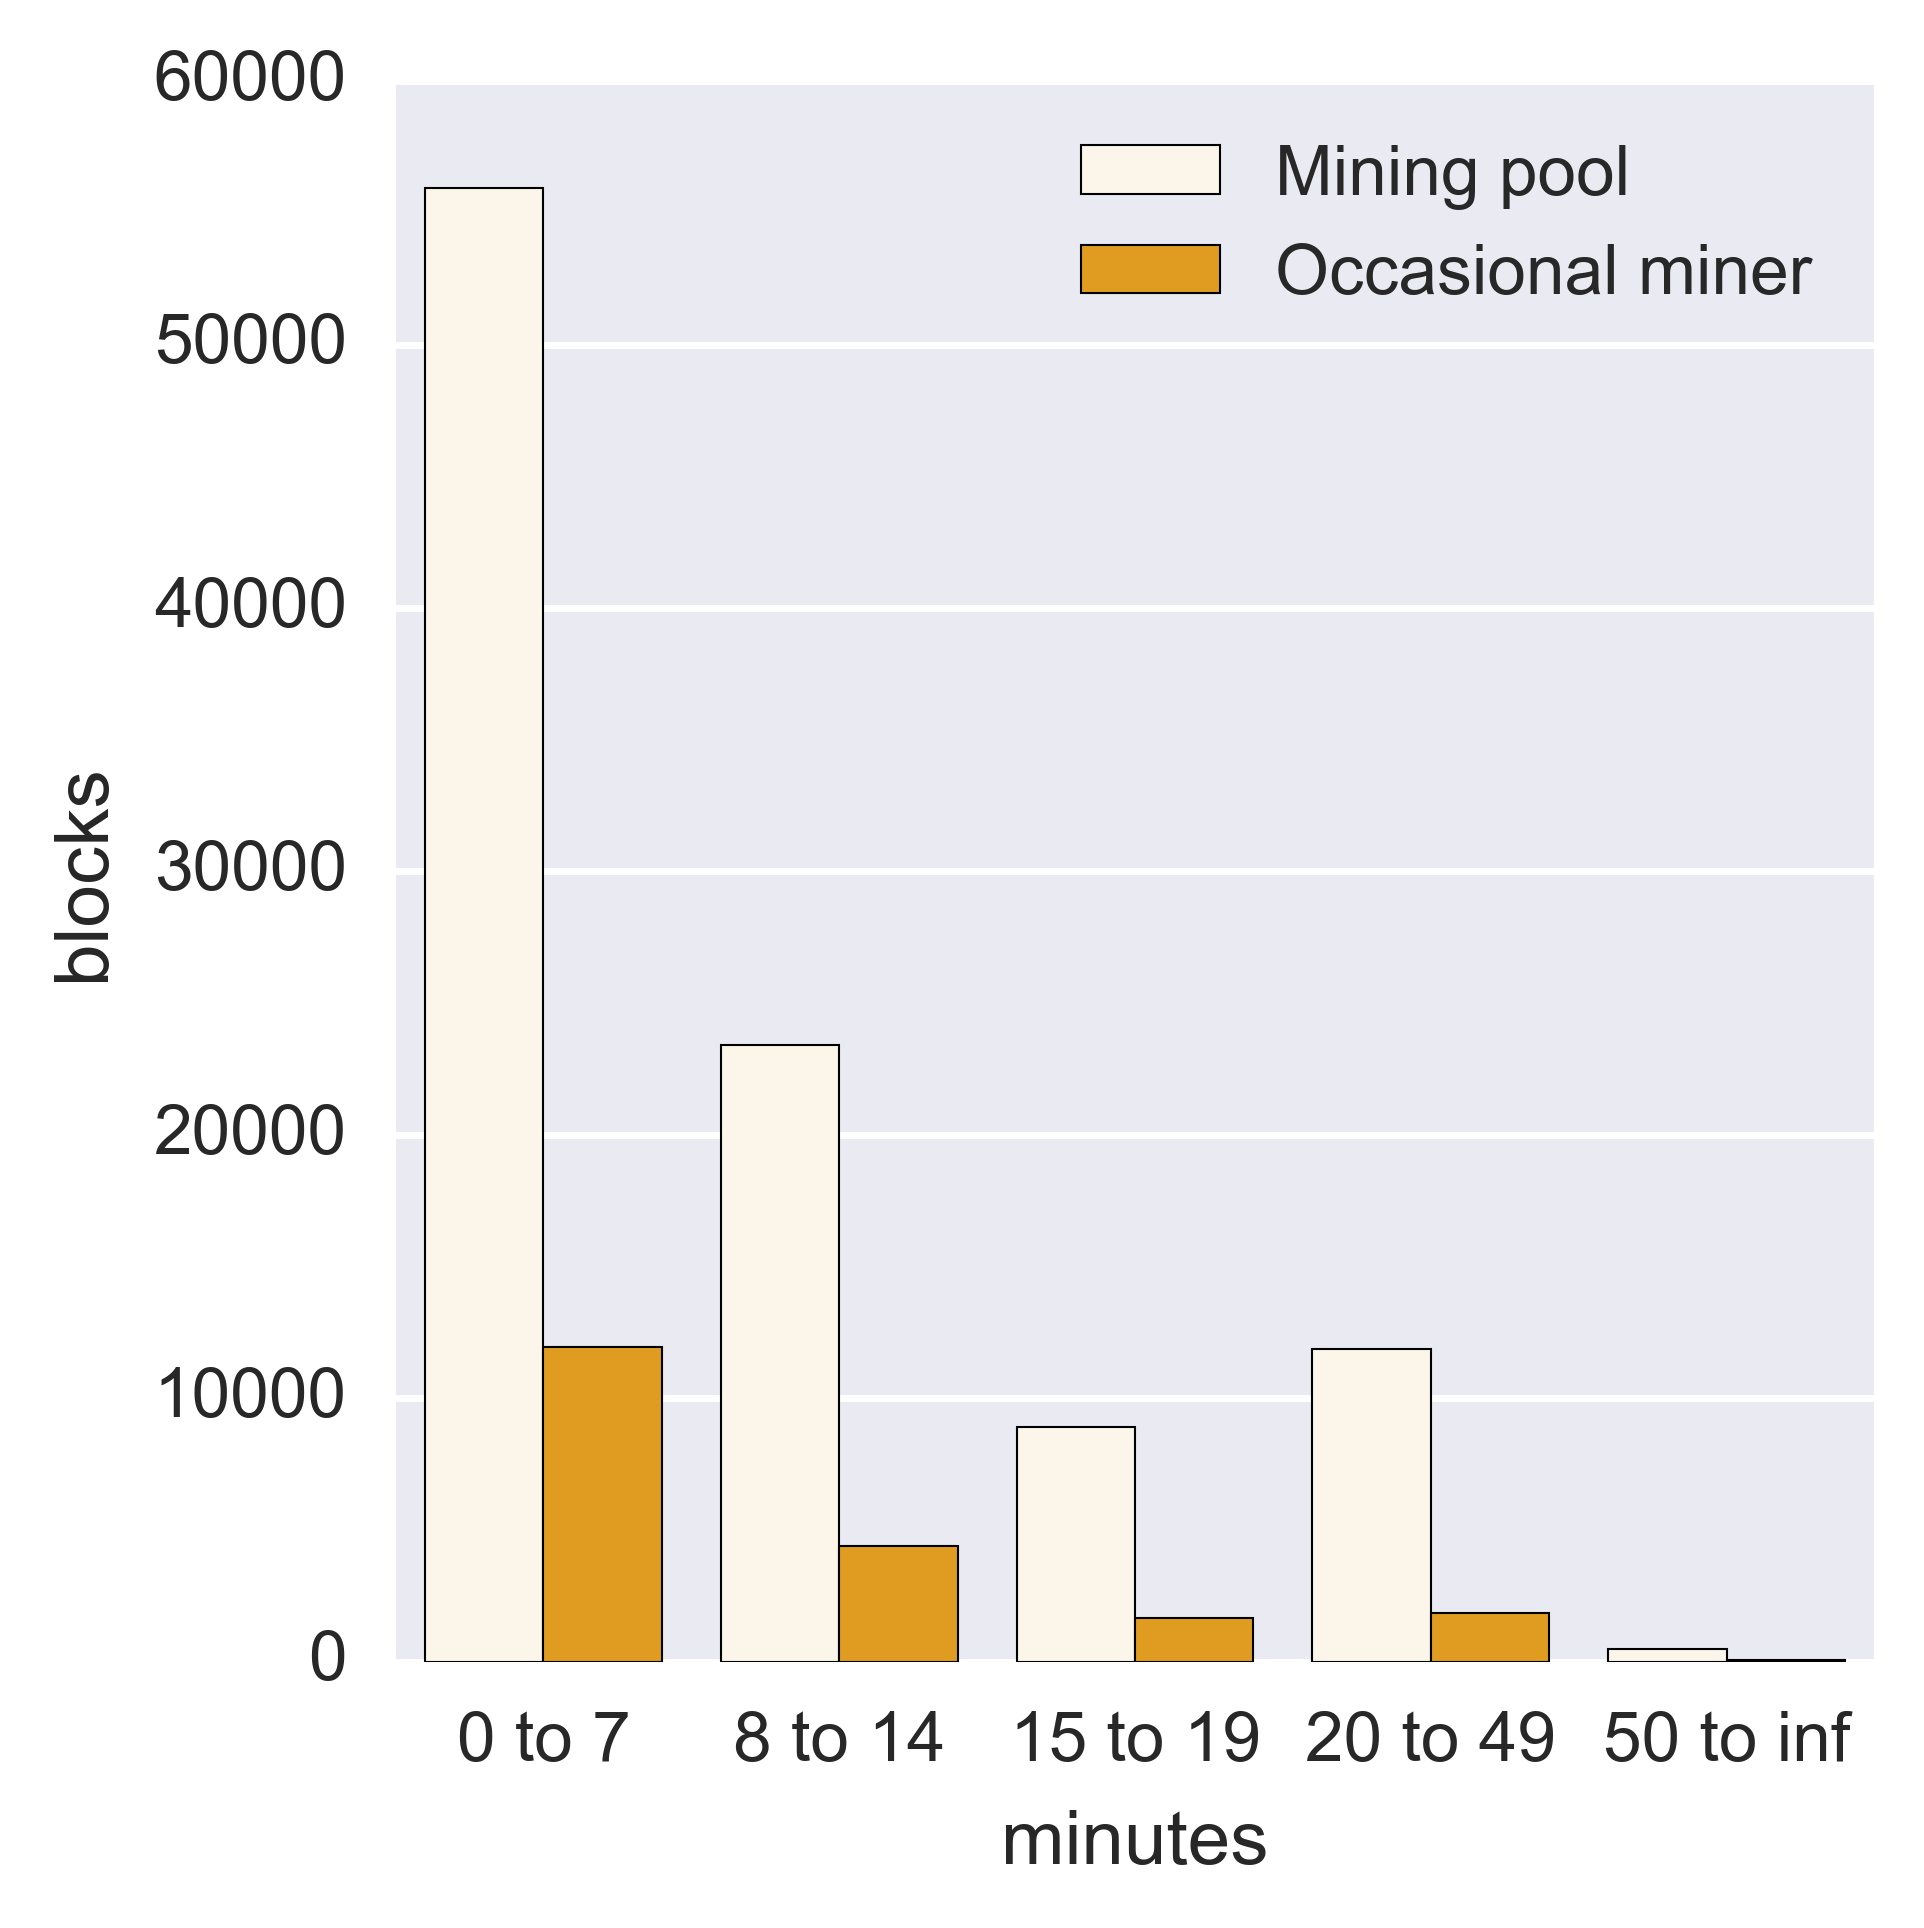
\includegraphics[width=1\textwidth]{img/creation_time_miners}
	\caption{Number of blocks mined by mining pools and occasional miners according their creation time.}
	\label{fig:creation_time_miners}
\end{figure}

\subsubsection{Block Size $Q$}
If the creation time $\mathcal{T}$ tends to have a fixed value, then
$Q$ plays a big role in throughput limitations.
Discussions on whether to increase the block size
limit or not are still ongoing
and this issue has been brought up
in several papers\,\cite{Rizun:2015:blocksizelimit, houy2014EOBTF}. Increasing
the block size limit leads to a bigger amount of transactions that could
be accepted at every block creation time, so we may think that
this could be the right solution to adopt
in order to increase the performance of the system.
Anyway there is a big controversy on this topic, and even the
biggest entities in the Bitcoin system do not agree to a solution.
Some such as CoinBase, Blockchain.info or BTC Guild, deem
that is beneficial to increase the block size,
some others like F2Pool or Ethereum
are neutral and other entities, for example GreenAddress, Bitrated or
Bitcoinpaygate, think that this is just pushing the problem a little
further and is not a good solution.
In our assumptions we also state that transaction fee
$t_f$ may decrease with an increment of the block size
limit, since transactions do not compete for space in the block
anymore. So a small block size will require higher
fees for fast confirmation, which will bring the
following pros ($+$) and cons ($-$)\,\cite{blocksizecontroversy}:
\begin{itemize}
	\item [$+$] It will no longer be cheap to spam transactions such as Satoshi Dice bets\,\cite{satoshidice}.
	\item [$+$] Fees will not be zero. This is eventually a necessity in order to encourage miners and secure the mining ecosystem.
	\item [$-$] Bitcoin may look unattractive to new users, having high fees.
	\item [$-$] Users pay higher fees.
\end{itemize}
We tested not only that the $t_f$ is related
to the increment of the block
size limit, but thanks to our evaluations presented in
Figures~\ref{fig:txs_fee_distribution}-\ref{fig:txs_feedensity_distribution},
we can state that from when the blockchain started
to become saturated in mid $2016$~(Figure~\ref{fig:block_size}),
$t_f$ but also the fee density $\rho$ had a big increment,
which is a sign that the blockchain is needing an urgent
change according to
avoid scalability problems.
Increasing the block size limit is one of the possible solutions,
but we have to consider that it might not only be good
for users, but also bad for miners.
The cost of mining increase along
with the block size, so receiving
no more fees from users would be costly effective
and lead to a centralization problem, since
larger blocks make full nodes more expensive to
operate, having then less hashers running full nodes,
discouraging in that way miners to join the network.
If we consider now the statement that block size
limit should be increased, these are the
arguments against it:
\begin{itemize}
	\item Orphan rate amplification.
	\item Damage to centralization.
	\item "Congestion" concerns can be solved with mempool improvements including transaction eviction.
	\item No amount of max block size would support all the world's future transactions on the main blockchain (various types of off-chain transactions are the only long-term solution).
\end{itemize}
In conclusion, even if we think that an immediate increment of the block size
is not the final solution to the scalability problem, we believe that
an immediate and temporary solution should be considered to
avoid network congestion, too high $t_l$ and drastic increment of $t_f$.
This temporary solution
might be the block size limit increment, especially if
big mining pools such as F2Pool claim that they could support
a maximum block size of $20$\,\gls{mb}\,\cite{blocksizecontroversy}.

\section{Performance}
\label{sec:performance}
Together with scalability, performance is one of our
main subject to study on Bitcoin and we can
say that it is highly related with scalability. In
Chapter~\ref{sec:unconfirmedtxs} we already
talked about throughput $\gamma$ and how it is
related to the block size $Q$ and block creation time
$\mathcal{T}$. We are now going to focus on
the Bitcoin network
performance from both, user side ($t_l$)
and system side ($\gamma$). Moreover,
our target by studying
transaction latency $t_l$ is to verify our assumptions
whether there is any relation between $t_f$ and $t_l$
during the whole period analyzed. These tests are
strictly related to the cost and fee problems
(Chapter~\ref{sec:feesandtolls}), and are important
to make users aware whether is possible
to pay for bandwidth in Bitcoin system, and
if yes, how to optimize their fee, $t_f$, according to get
faster $t_l$.

\subsection{Throughput $\gamma$}
\label{sec:throughput}
As we state in Chapter~\ref{sec:unconfirmedtxs}, $\gamma$
is highly dependent on $Q$ and $t_q$, but also related
to $\mathcal{T}$. Block size limit can set the
number of transactions the network can confirm
per block, thereby the throughput of the whole Bitcoin
network. In Figure~\ref{fig:throughput} we show how
throughput has changed during the years. We want to clarify that
in $2013$ the system was not performing less, there were just less
transactions to process, roughly fifty thousands per day, and
only when the blocks started to get saturated in mid $2016$,
the system began to use its maximum throughput capacity of
$\sim$$3$-$4$ transactions per second. However,
if compared to centralized trusted-oriented
system, throughput is extremely low.
Assumptions in Table~\ref{tab:assumptions} about
throughput were correct, and in order to have a higher
throughput, $Q$ needs to be bigger,
$\mathcal{T}$ lower, or both.
However, an increment on $\gamma$ will bring
a raise on the cost $\langle C\rangle$ if $Q$ is changed, and
a growth of $\mathbb{P}_{orphan}$ with also repercussions
on $\langle C\rangle$ if $\mathcal{T}$ is lowered.
\begin{figure}[h]
	\centering
	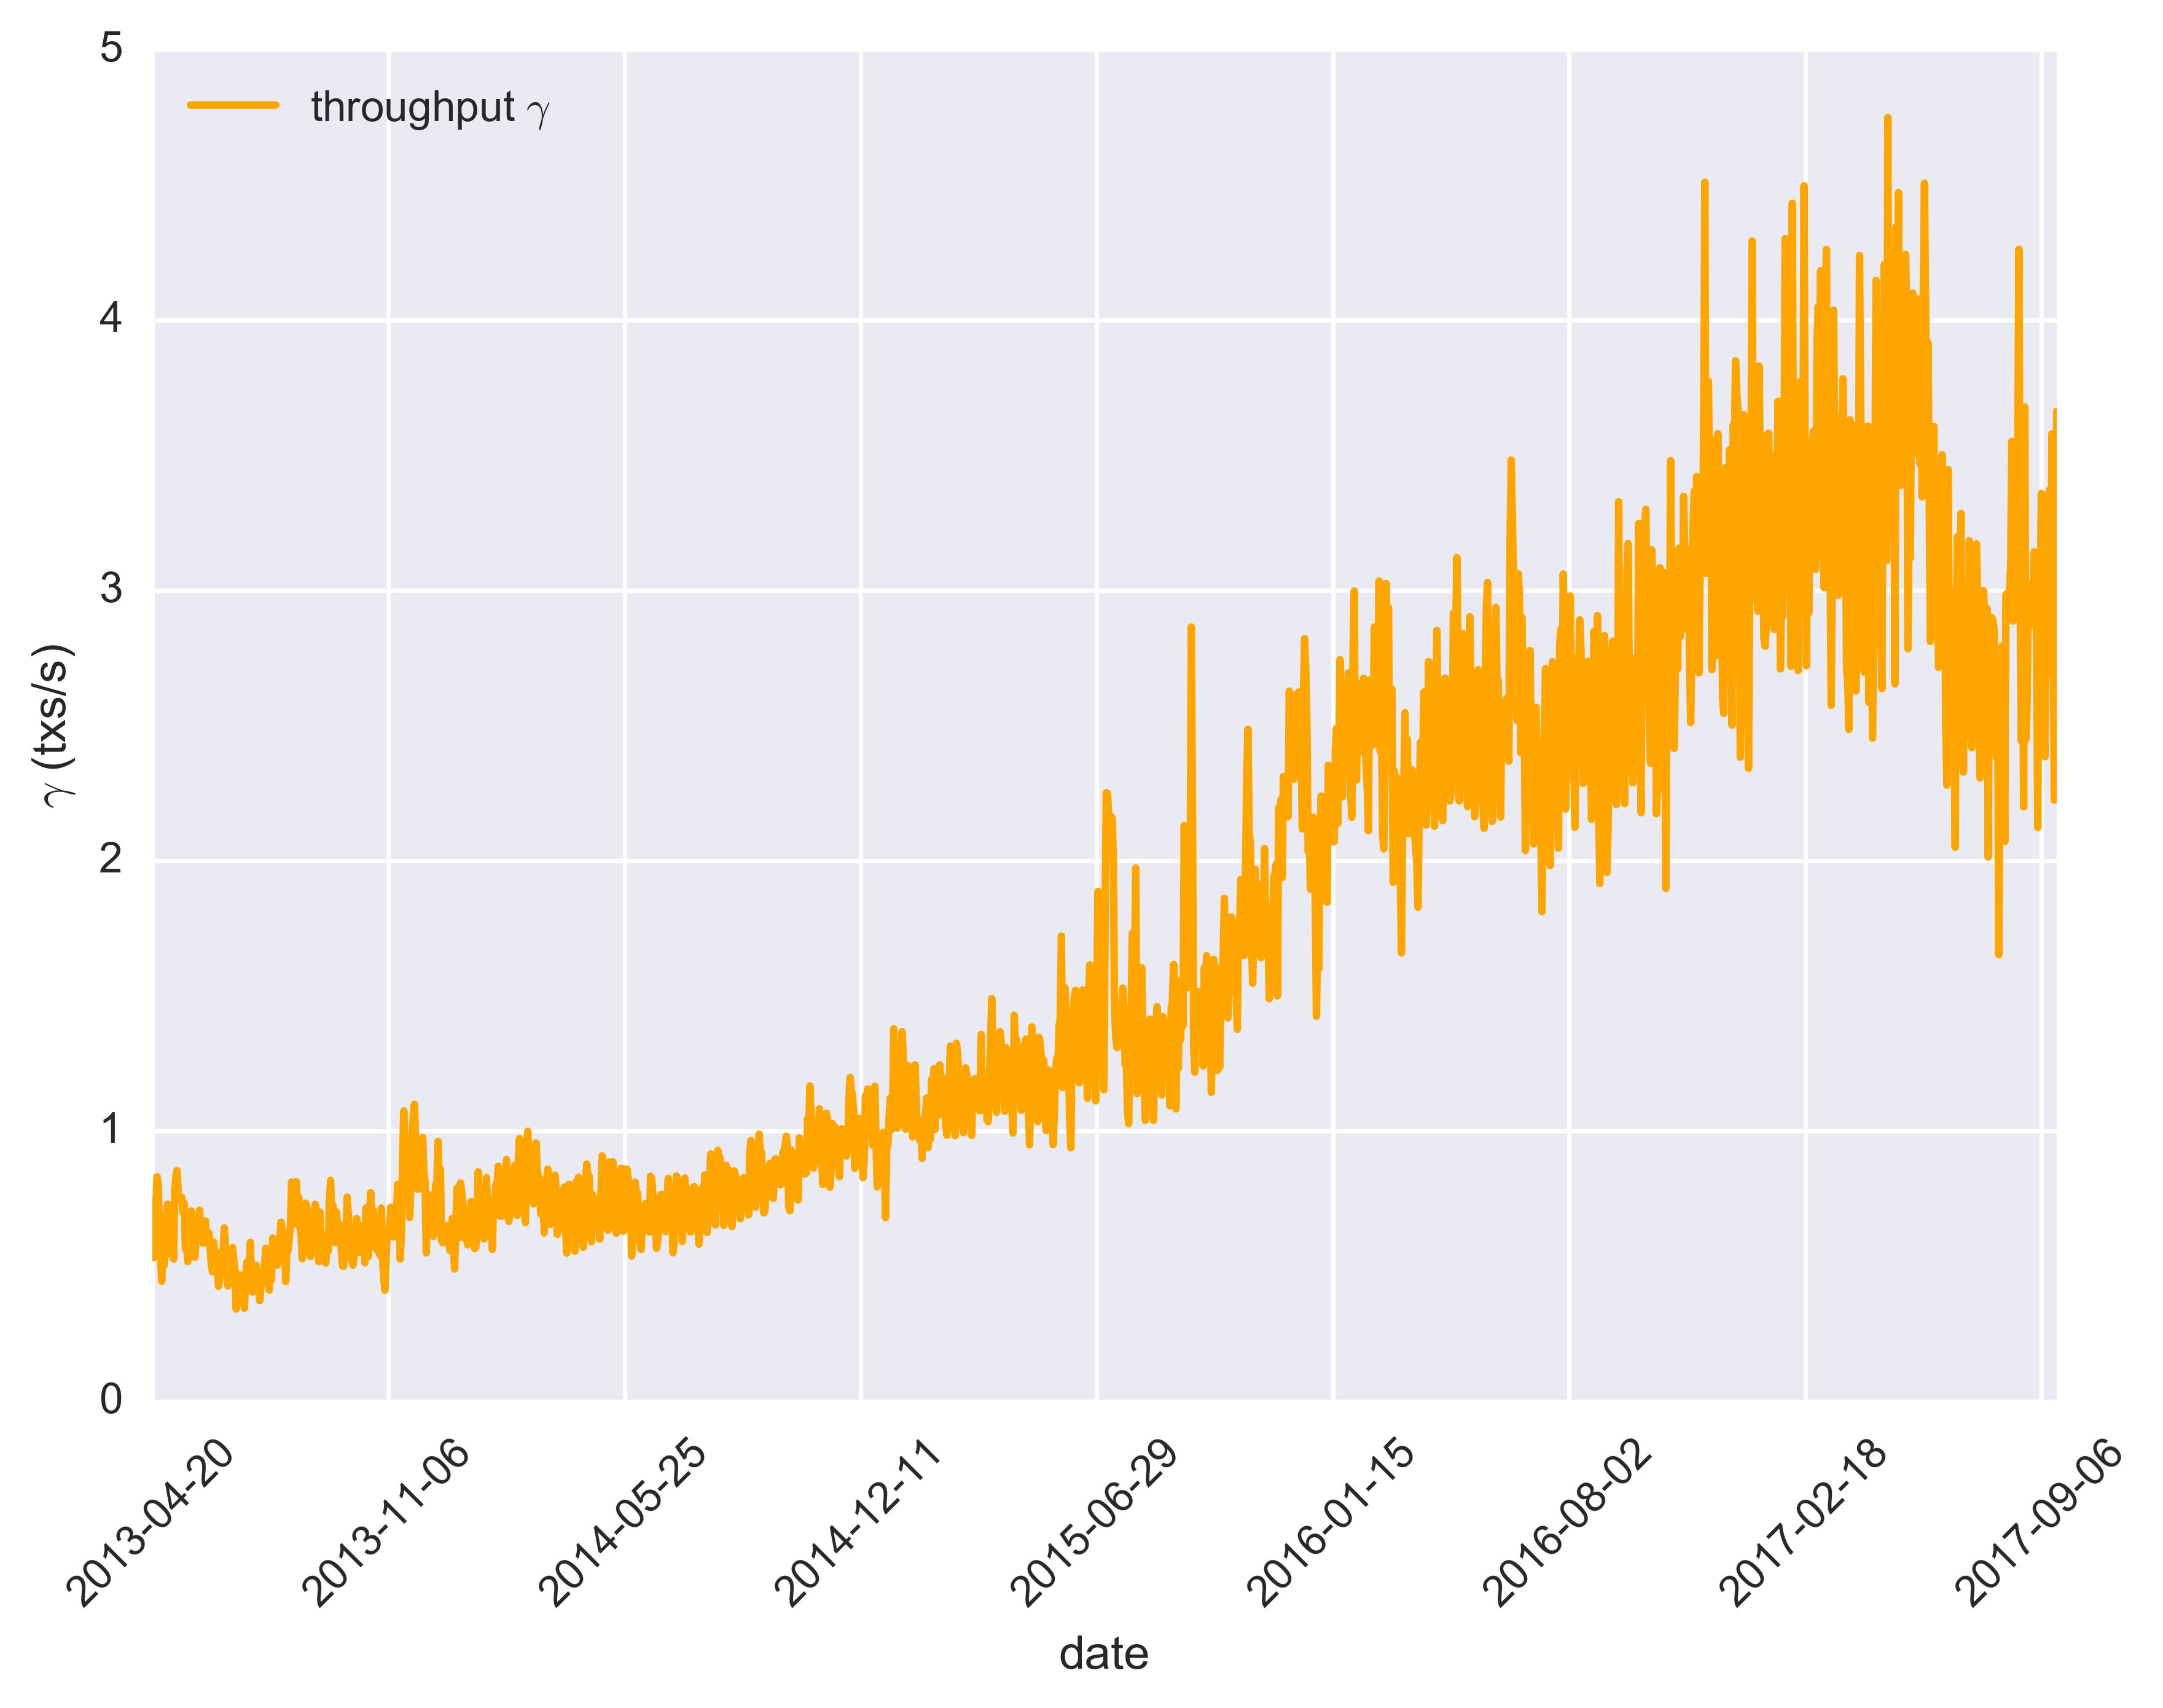
\includegraphics[width=1\textwidth]{img/throughput}
	\caption{Throughput ($\gamma$) of the Bitcoin blockchain calculated in a period from $2013$ until $2017$.}
	\label{fig:throughput}
\end{figure}

\subsection{Transaction Latency $t_l$}
\label{sec:txslatency}
Another important aspect of performance
regards the bandwidth that Bitcoin could offer to users.
We considered the latency $t_l$ of every
transaction, which is the time necessary for
$t$ to be approved by the network. We want to find
out how and why $t_l$ and $t_f$
changed during these years pointing out, if any,
the relation between these two attributes, so that
users are aware while paying a certain $t_f$, in how much
time approximately their transactions will be approved
and confirmed by the network.
We observed that from $2013$ to $2017$, while the average
transaction latency did not vary much and was stable
at $\sim$$15$ minutes, the fee paid from users to the miners
has undergone a relevant raise, from an average of $0.0001$\,\bitcoinA~to
$0.0004$\bitcoinA, with peaks of $0.0012$\,\bitcoinA~in $2017$,
where the Bitcoin price is
also $2000$ times higher than in $2013$.
In our assumptions (Table~\ref{tab:assumptions})
we show how $t_l$ could be affected
by other attributes in the system.
Assumptions on $\tau$ and $\gamma$ are immediate,
so the transaction latency will increase if the
propagation time grows and will decrease if the throughput
gets higher.
Other assumptions required a deeper study, for example,
we analyzed the relation between
block size $Q$ and transaction latency $t_l$. We divided
the block size in categories, then plotted these
categories in relation with $t_l$ and grouped the whole
dataset by year, Figure~\ref{fig:blocksize_latency}.
As we suspected, during the years,
whenever there was an increment on the block size, transaction
latency had a drop. In $2016$ when we had the final
increment to $1$\,\gls{mb}, the latency started
to become incredibly low, while in $2017$ when the blocks
started to get saturated we have a latency up to
$9$ times higher, plus, smaller blocks in $2017$ verify
a much higher transaction latency since they include less
transactions than the amount that need to be approved.
\begin{figure}[h]
	\centering
	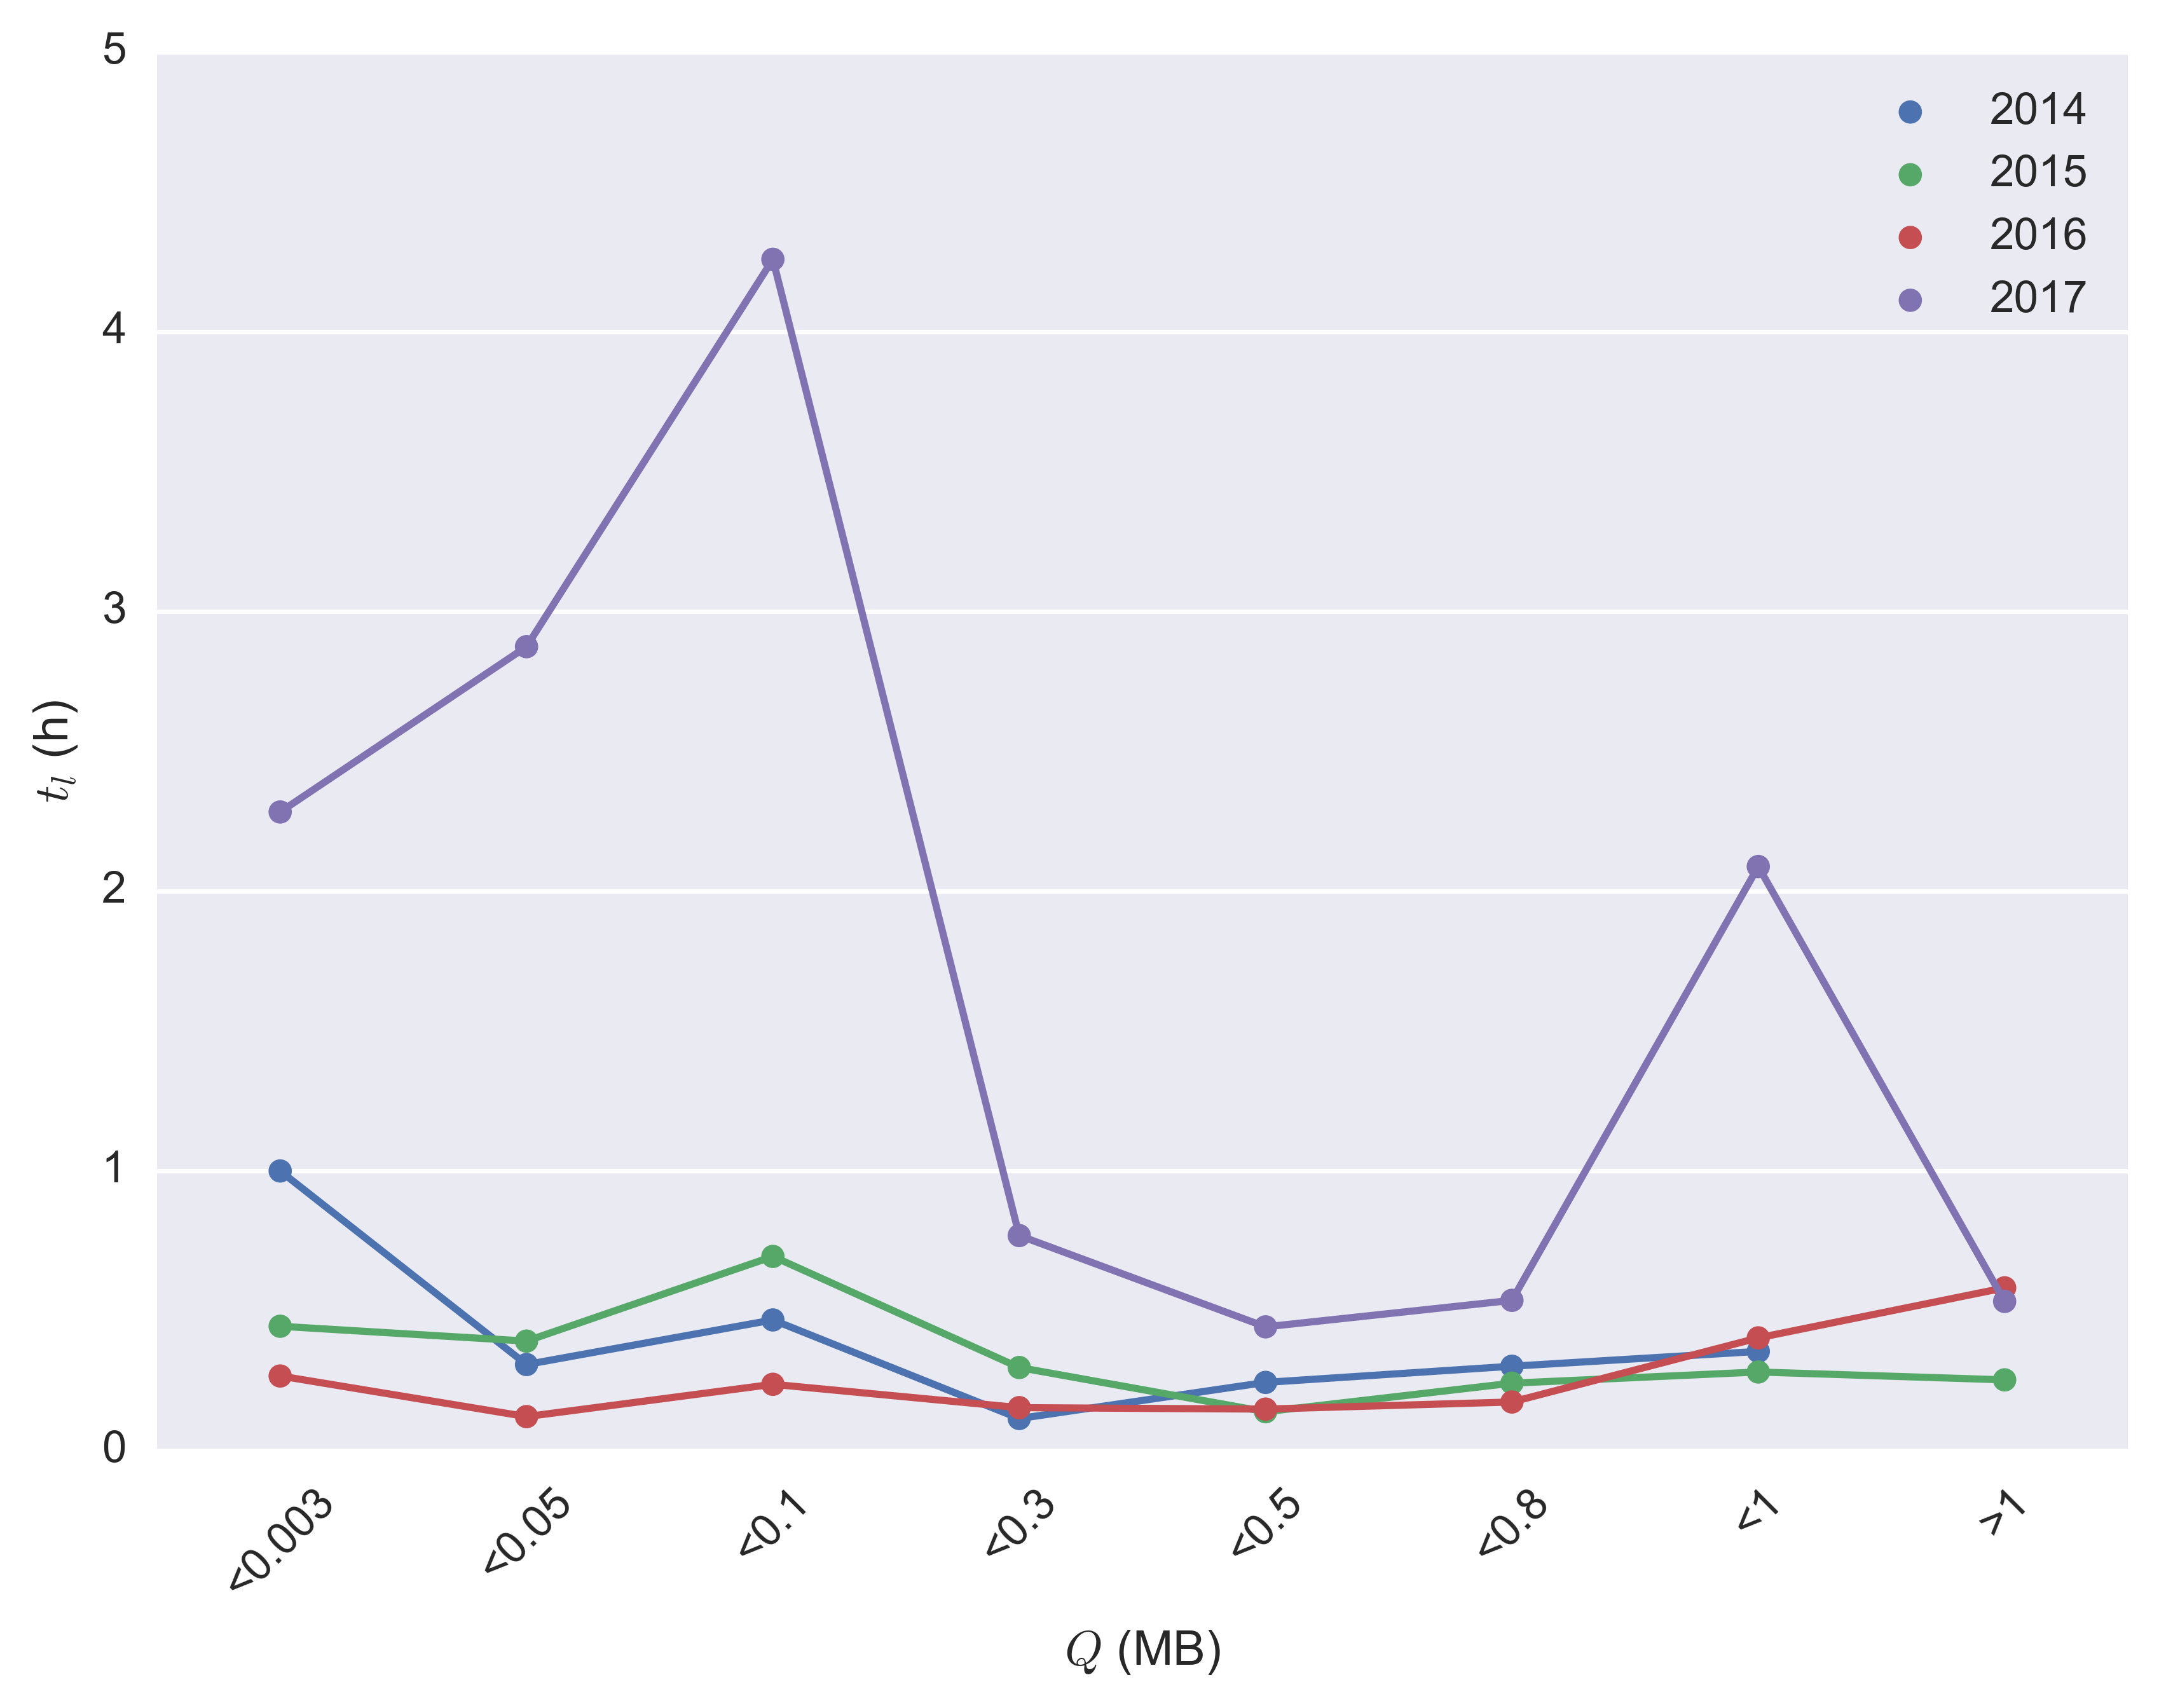
\includegraphics[width=1\textwidth]{img/blocksize_latency}
	\caption{Relation between $t_l$ and $Q$ from $2014$ until $2017$.}
	\label{fig:blocksize_latency}
\end{figure}

Not much intuitive and more difficult to study was the
relation between $t_l$ fee and $t_f$. According to the
analysis made on $t_f$ we categorized the fee paid
from users to miners and then we split the data frame per year.
Table~\ref{tab:fee_categorized} enhance this categorization and
Figure~\ref{fig:fee_latency} shows the plot generated while analyzing
more than one hundred twenty million of transactions from $2013$ to $2017$.
\begin{table}
	\centering
	\caption{Table representing the results in Figure~\ref{fig:fee_latency},
	showing how $t_l$ might vary for each category of fee.}
	\label{tab:fee_categorized}
	\begin{tabular}{|p{2.5cm}|p{4.5cm}|p{3cm}|} \hline
		\textbf{Fee category}&\textbf{$t_f$ value (\bitcoinA)}& \textbf{$t_l$ variation (h)}\\
		\hline
		$0$&$t_f = 0$& $1$ to $33$\\
		\hline
		$<$$0.0002$&$0\leq t_f < 0.0002$&$0$+ to $5$+\\
		\hline
		$<$$0.0004$&$0.0002\leq t_f < 0.0004$&$0$+ to $2.5$\\
		\hline
		$<$$0.0006$&$0.0004\leq t_f < 0.0006$&$0$+ to $1.5$\\
		\hline
		$<$$0.0008$&$0.0006\leq t_f < 0.0008$&$0$+ to $1$\\
		\hline
		$<$$0.001$&$0.0008\leq t_f < 0.001$&$0$+ to $1$\\
		\hline
		$<$$0.01$&$0.001\leq t_f < 0.01$&$0$+ to $1$\\
		\hline
		$<$$0.1$&$0.01\leq t_f < 0.1$&$0$+ to $1.5$\\
		\hline
		$>$$0.1$&$t_f \geq 0.1$&$0$+ to $2$\\
		\hline
	\end{tabular}
\end{table}
As Table~\ref{tab:fee_categorized} and Figure~\ref{fig:fee_latency} enhance,
the fee paid from users has a bigger impact year by year on the
available bandwidth the system offers. Our assumptions about this relation
were right, and especially after the blocks started to get saturated in
mid $2016$ there was big change in the way miners include transactions.
If during $2013$ and $2014$, miners and mining pools tended to include in blocks
a compromise between fee and waiting time, in $2017$ miners tend to
completely ignore $0$-fee transactions. This could be good to
avoid transaction spamming and it is good for miners that are gaining
more from mining, since the block reward is halved every two
hundred ten thousand blocks.
On the other hand, impatient users need to pay a higher fee to
see their transactions approved faster.
\begin{figure}[h]
	\centering
	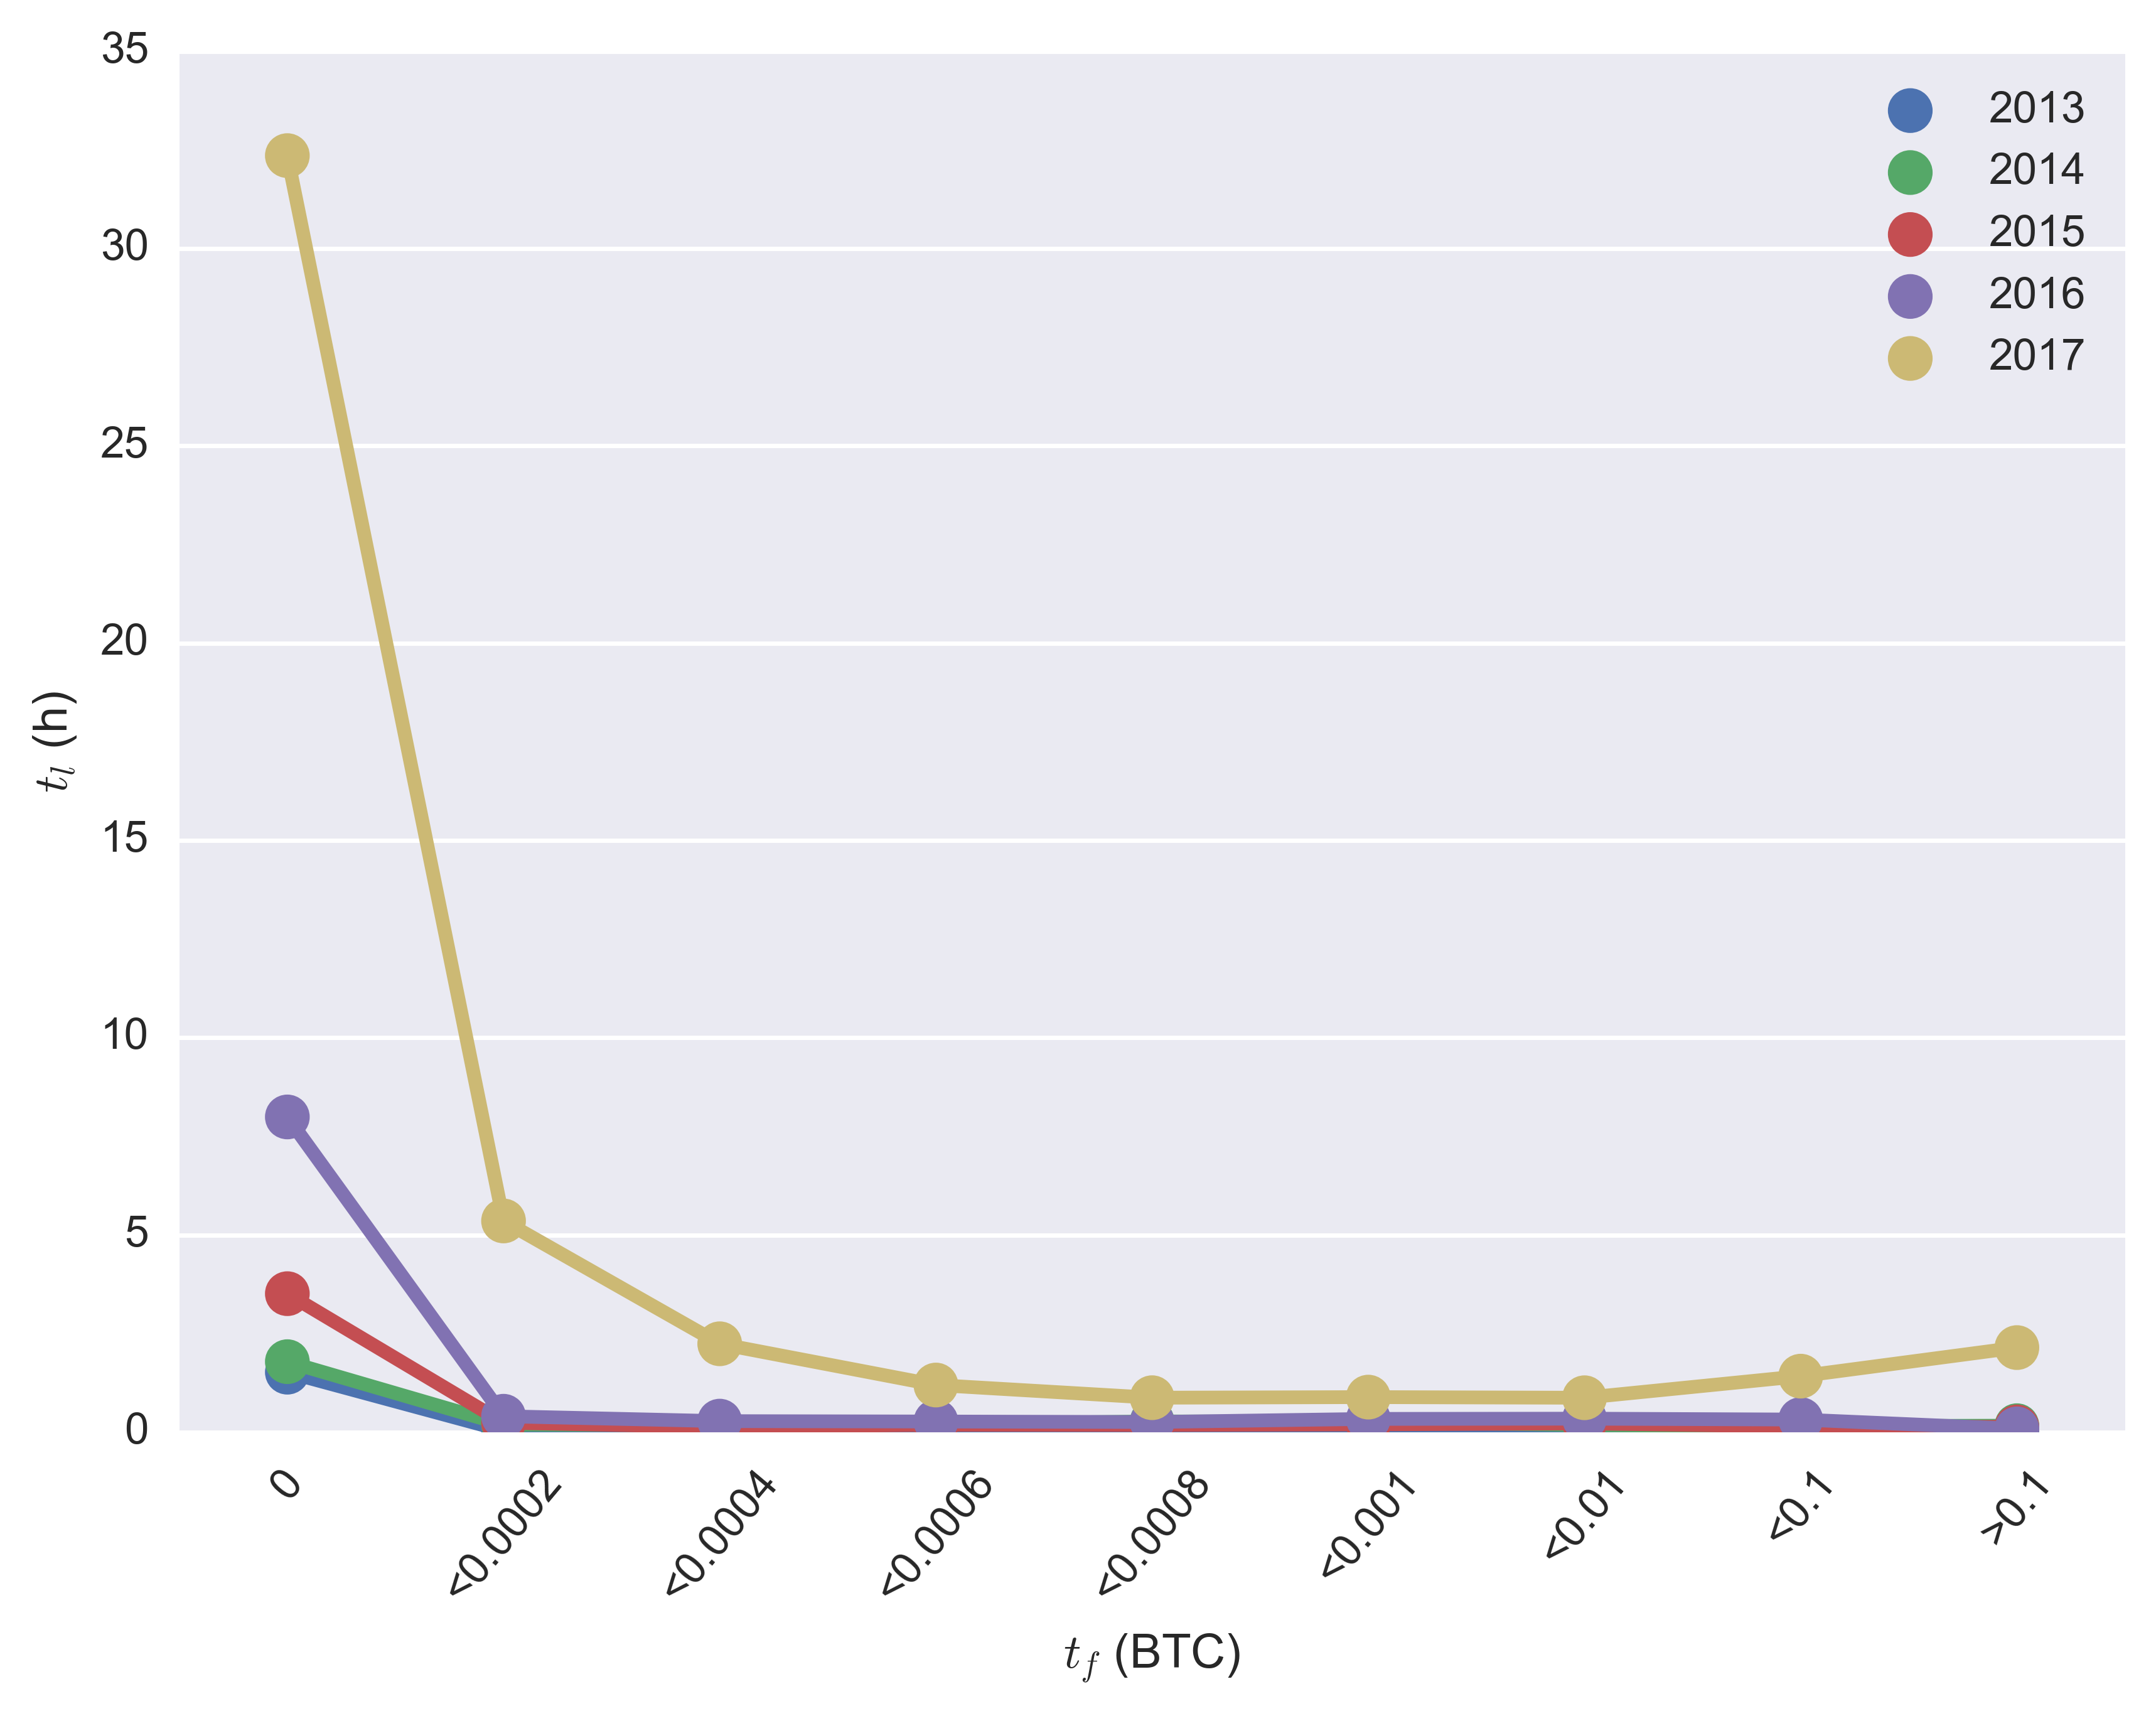
\includegraphics[width=1\textwidth]{img/fee_latency}
	\caption{Relation between $t_l$ and $t_f$ grouped by year.}
	\label{fig:fee_latency}
\end{figure}
Furthermore, we can state that in $2017$,
$0$-fee transactions have a latency of $\sim$$33$\,hours,
$4$ times bigger than $2016$, $8$ times than $2015$,
and more than $16$
times bigger than $2013$ and $2014$, which means that the problem
of block saturation has been partially considered by some miners
with $0$-fee transactions eviction.
Today miners are using fork mechanism such
as \emph{BitcoinABC}\,\cite{bitcoinabc} and they tend to exclude
$0$-fee transactions, so users should be aware that,
a $0$-fee transaction might not be mined at all.

\section{Costs and Fees}
\label{sec:feesandtolls}
This Section aims to show the changes in tips and tolls in Bitcoin
system from $2013$ to $2017$.
Möser and Böhme\,\cite{Moser2015}, claim that
the hard size limit still does not affect the level of the fee paid.
We want to enhance instead, that nowadays the saturation
problem significantly drives the fee paid
from users in order to get more bandwidth
or to be accepted at all. Furthermore, at the time
of analysis ($2015$), Bitcoin claimed that the fees were
lower than $0.1\%$ while today
we analyzed (Figure~\ref{fig:fee_input_miners})
to have an average
percentage of $0.25$\%,
which is more than the double.
Plus we want to consider the mining cost
for miners, from what it is driven and how it will change
in the past years.
When we talk about fees and tolls we might refer both to miner's
profit and users' benefits.

\subsection{Miners' Profit}
\label{sec:minersprofit}
The study of how profitable is mining for miners,
is complex and a lot of
data analysis and manipulation is required. Knowledge
regarding electricity consumption, mining hardware, and
cost of hashing is needed, and a deep study and data analysis
on how the Bitcoin hashing rate and the Bitcoin price in \gls{usd}
changed during the years has to be taken into consideration.
Making assumptions about mining costs/profits might be
difficult due to the information withheld from mining pools.
We think though, that this is an important concern and it has
to be addressed and studied, since the block reward is even
halved every two hundred ten thousand
blocks, and miners should find another
way to profit from mining. Solutions for miners might be to
additionally charge users with higher fees or to optimize
their mining profit $\langle \Pi \rangle$ by analyzing
the costs $\langle C \rangle$ and the revenue $\langle V \rangle$
over time. We refer to Equations~\ref{eq:hashingcost},
\ref{eq:expectedrevenue},
\ref{eq:minerprofiteq} in order to calculate
$\langle C \rangle$, $\langle V \rangle$ and $\langle \Pi \rangle$.
For the reckoning
we had to adapt our data and formulas to the
Bitcoin price and Bitcoin total hash rate $H$ at the time
when data were generated. To do so, we extracted our
time information from $D$, collected \gls{json} data
regarding $H$ and Bitcoin price from \url{blockchain.info}
and finally fitted them in order to get $\langle \Pi \rangle$,
$\langle C \rangle$ and $\langle V \rangle$.
Equation~\ref{eq:minerprofiteq} gives us information
in order to calculate $\langle C \rangle$ and
$\langle V \rangle$, and we use
a propagation time of $\tau = 15.7$\,seconds,
considering in that way a scenario with
an average block size of $1$\,\gls{mb} and
a $50$\% propagation; in addition, we contemplate
an electricity cost of $0.04$\,\$/kWh (Chinese price, since
AntPool is a Chinese mining pool), and
examining the most powerful
mining hardware on the market for Bitcoin,
AntMiner~S$9$\,\cite{antminerS9}, having a hashing power
of $h = 14,000,000$\,MH/s and a consumption
of $1375$\,W, with an overall cost per hash of
$\eta = 1.091 \times 10^{-18}$\,\$/H.
A similar analysis on electricity consumption and
cost of mining was made by Croman et al.\,\cite{croman2016}
in $2016$.
For our calculations, we only considered transactions from
late $2016$ and $2017$, when Bitcoin's price was already over
$1000$\,\$, before that, data might contain too many
outliers due to huge differences in Bitcoin's hashing
rate and Bitcoin price, and they could drive the
analysis to an incorrect status.
\begin{figure}[h]
	\centering
	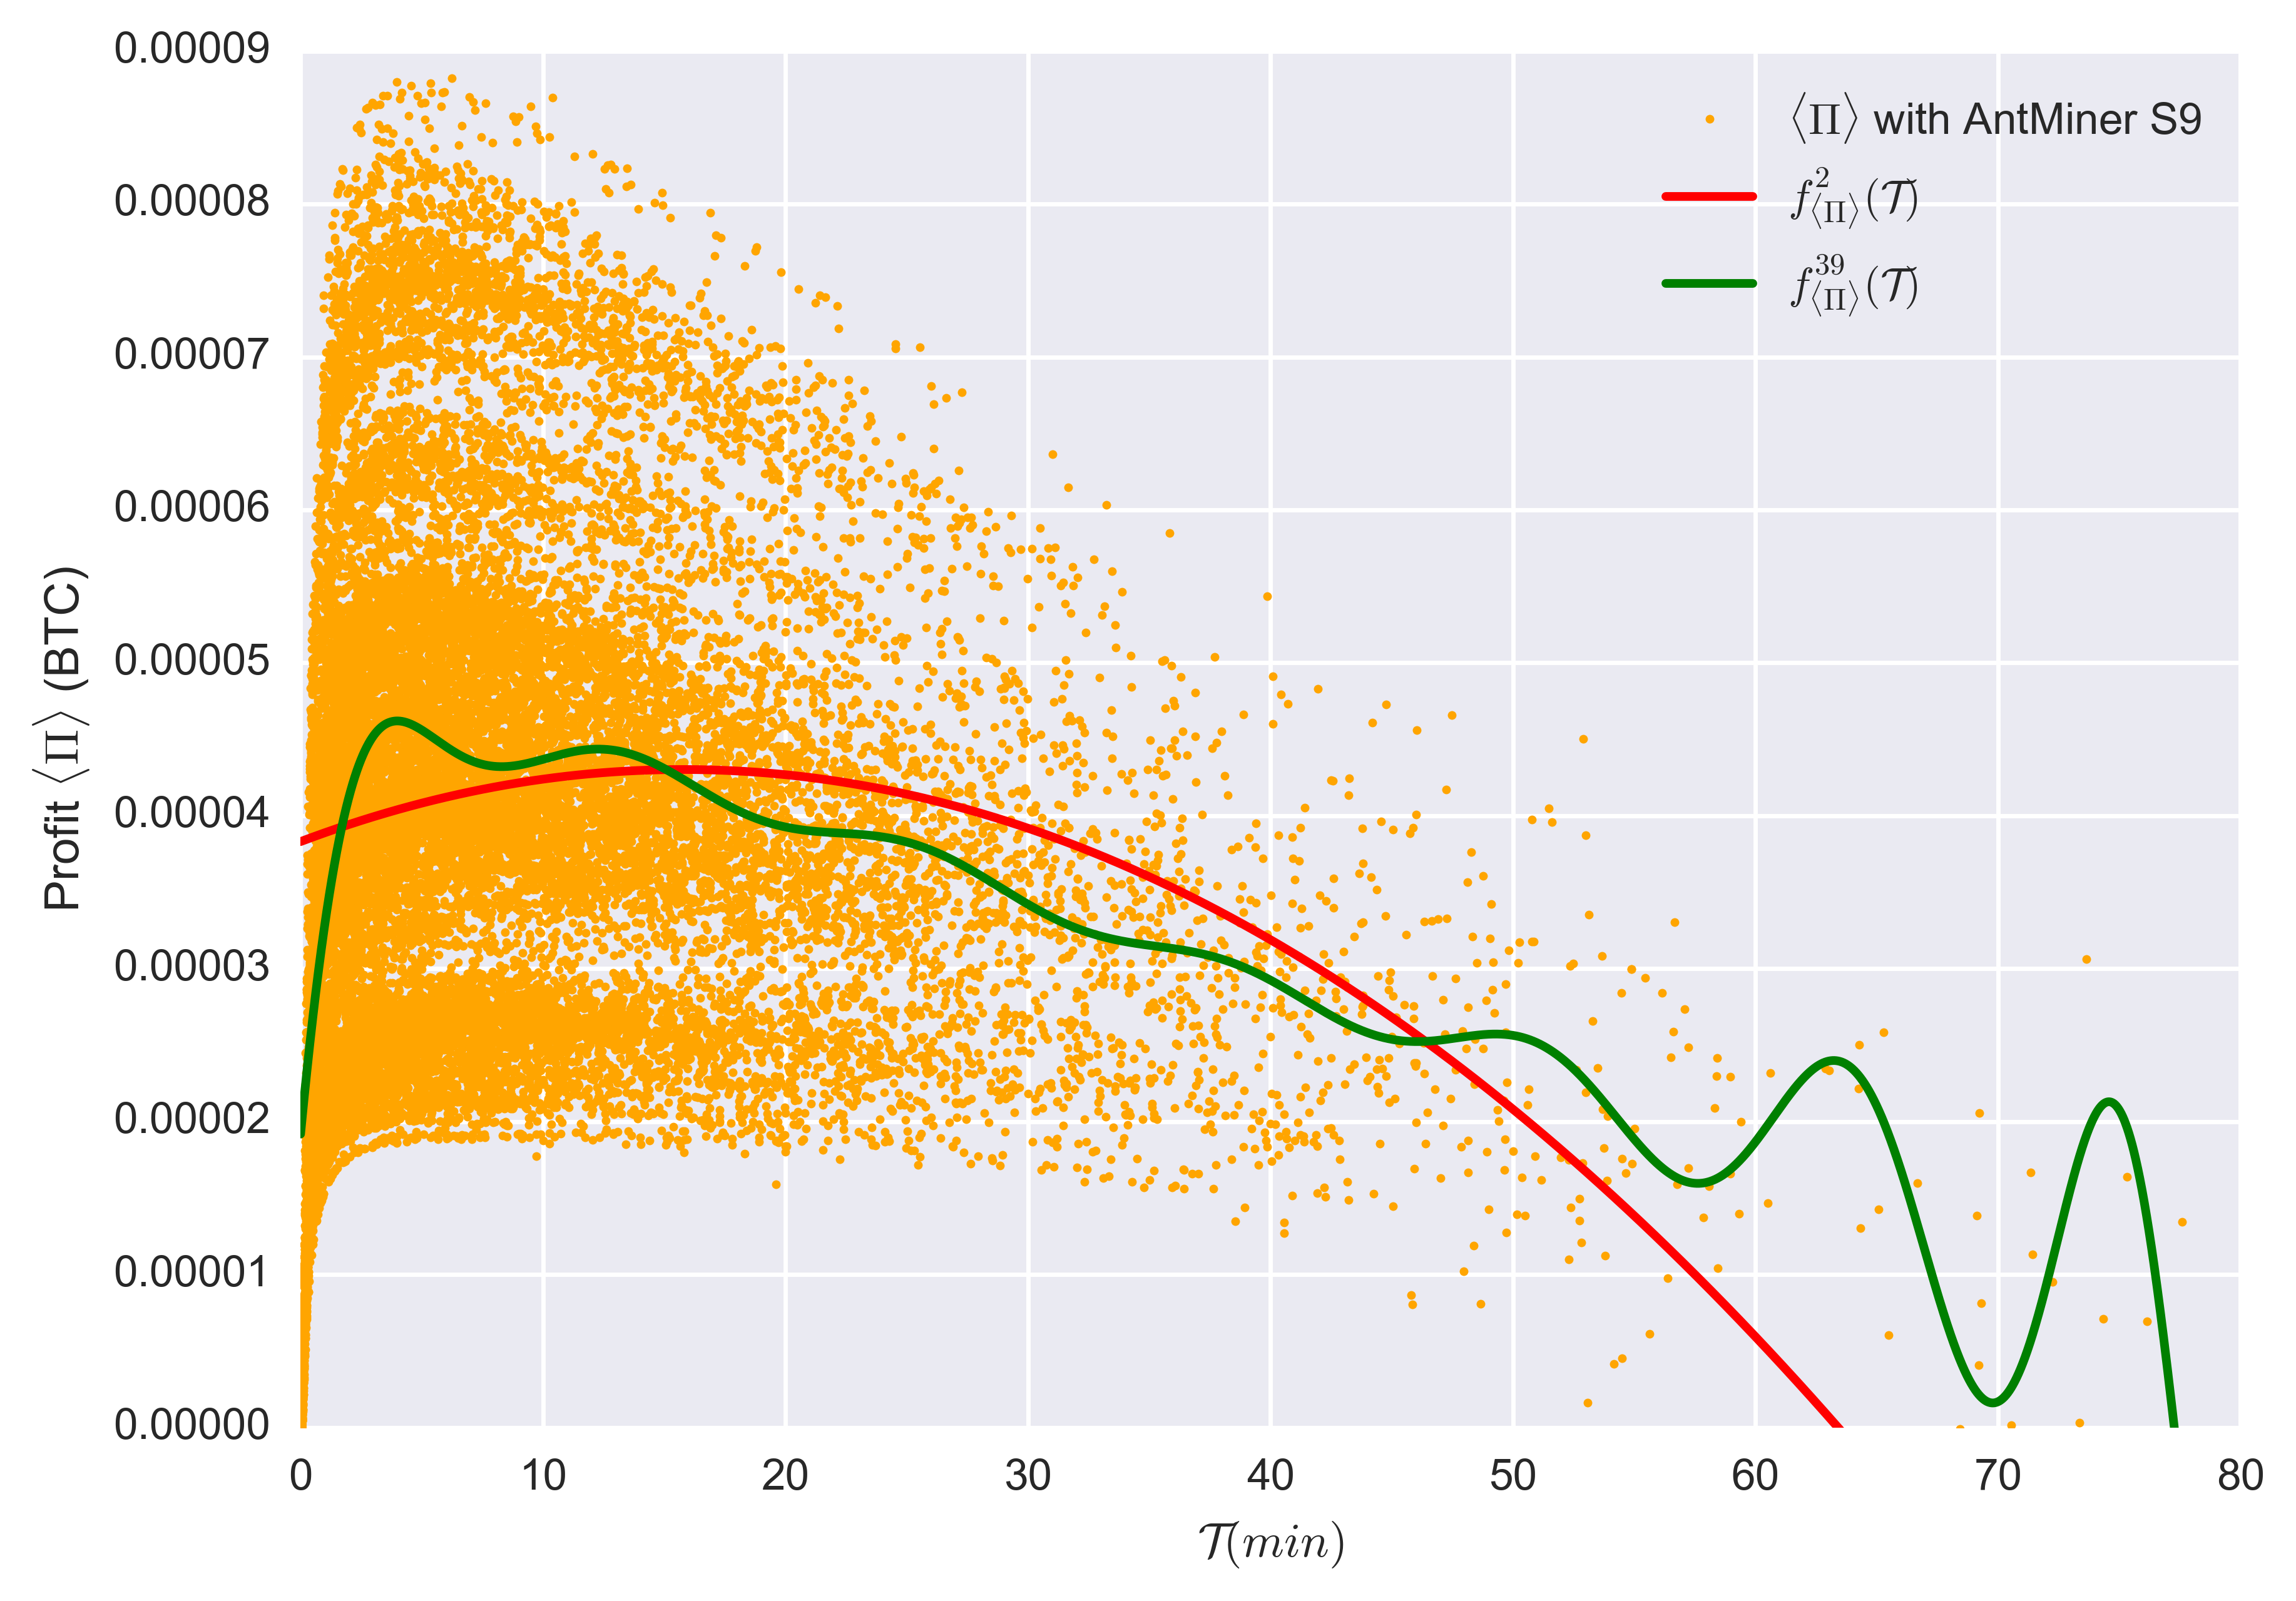
\includegraphics[width=1\textwidth]{img/profit_creation_time}
	\caption{Profit $\langle \Pi \rangle$ in relation with block creation time $\mathcal{T}$
		while mining with AntMiner~S$9$ from
		$2015$ until $2017$.}
	\label{fig:profit_creation_time}
\end{figure}
Figure~\ref{fig:profit_creation_time}, shows how the
miner's profit is related with the block creation time and how,
after $15$-$20$\,minutes, the miner starts to decrease its profit.
This is caused by the constant growth of the cost
necessary to mine a block, $\langle C \rangle$,
which is directly proportional to the cost per hash $\eta$ and
the block creation time $\mathcal{T}$.
Is important to enhance that Figure~\ref{fig:profit_creation_time} shows
the profit $\langle \Pi \rangle$ for a single miner,
using AntMiner~S$9$, and that in a real
case scenario we might have hundreds of
computers working together, so the possibilities
to find a new block are much higher and
the revenue $\langle V \rangle$ is
accordingly bigger, having then
much greater profit that needs to be shared
among all the miners.

Furthermore, as we will see in
Chapter~\ref{sec:userbenefits}, miners most likely
include transactions with a higher fee density ($\rho$),
so if users are not willing to pay more fee,
once all the best $\rho$-wise
transactions are already included in the new upcoming block
but $Q$ is not reached yet, miners
have to include lower fee density
transactions, having in that way a loss in their profit.
So if we look at it from a miner's prospective, the increment
of $Q$ might not be the best choice in the long run, unless the
fees are standardized in a way that every
miner has a guaranteed profit.
\begin{figure}[h]
	\centering
	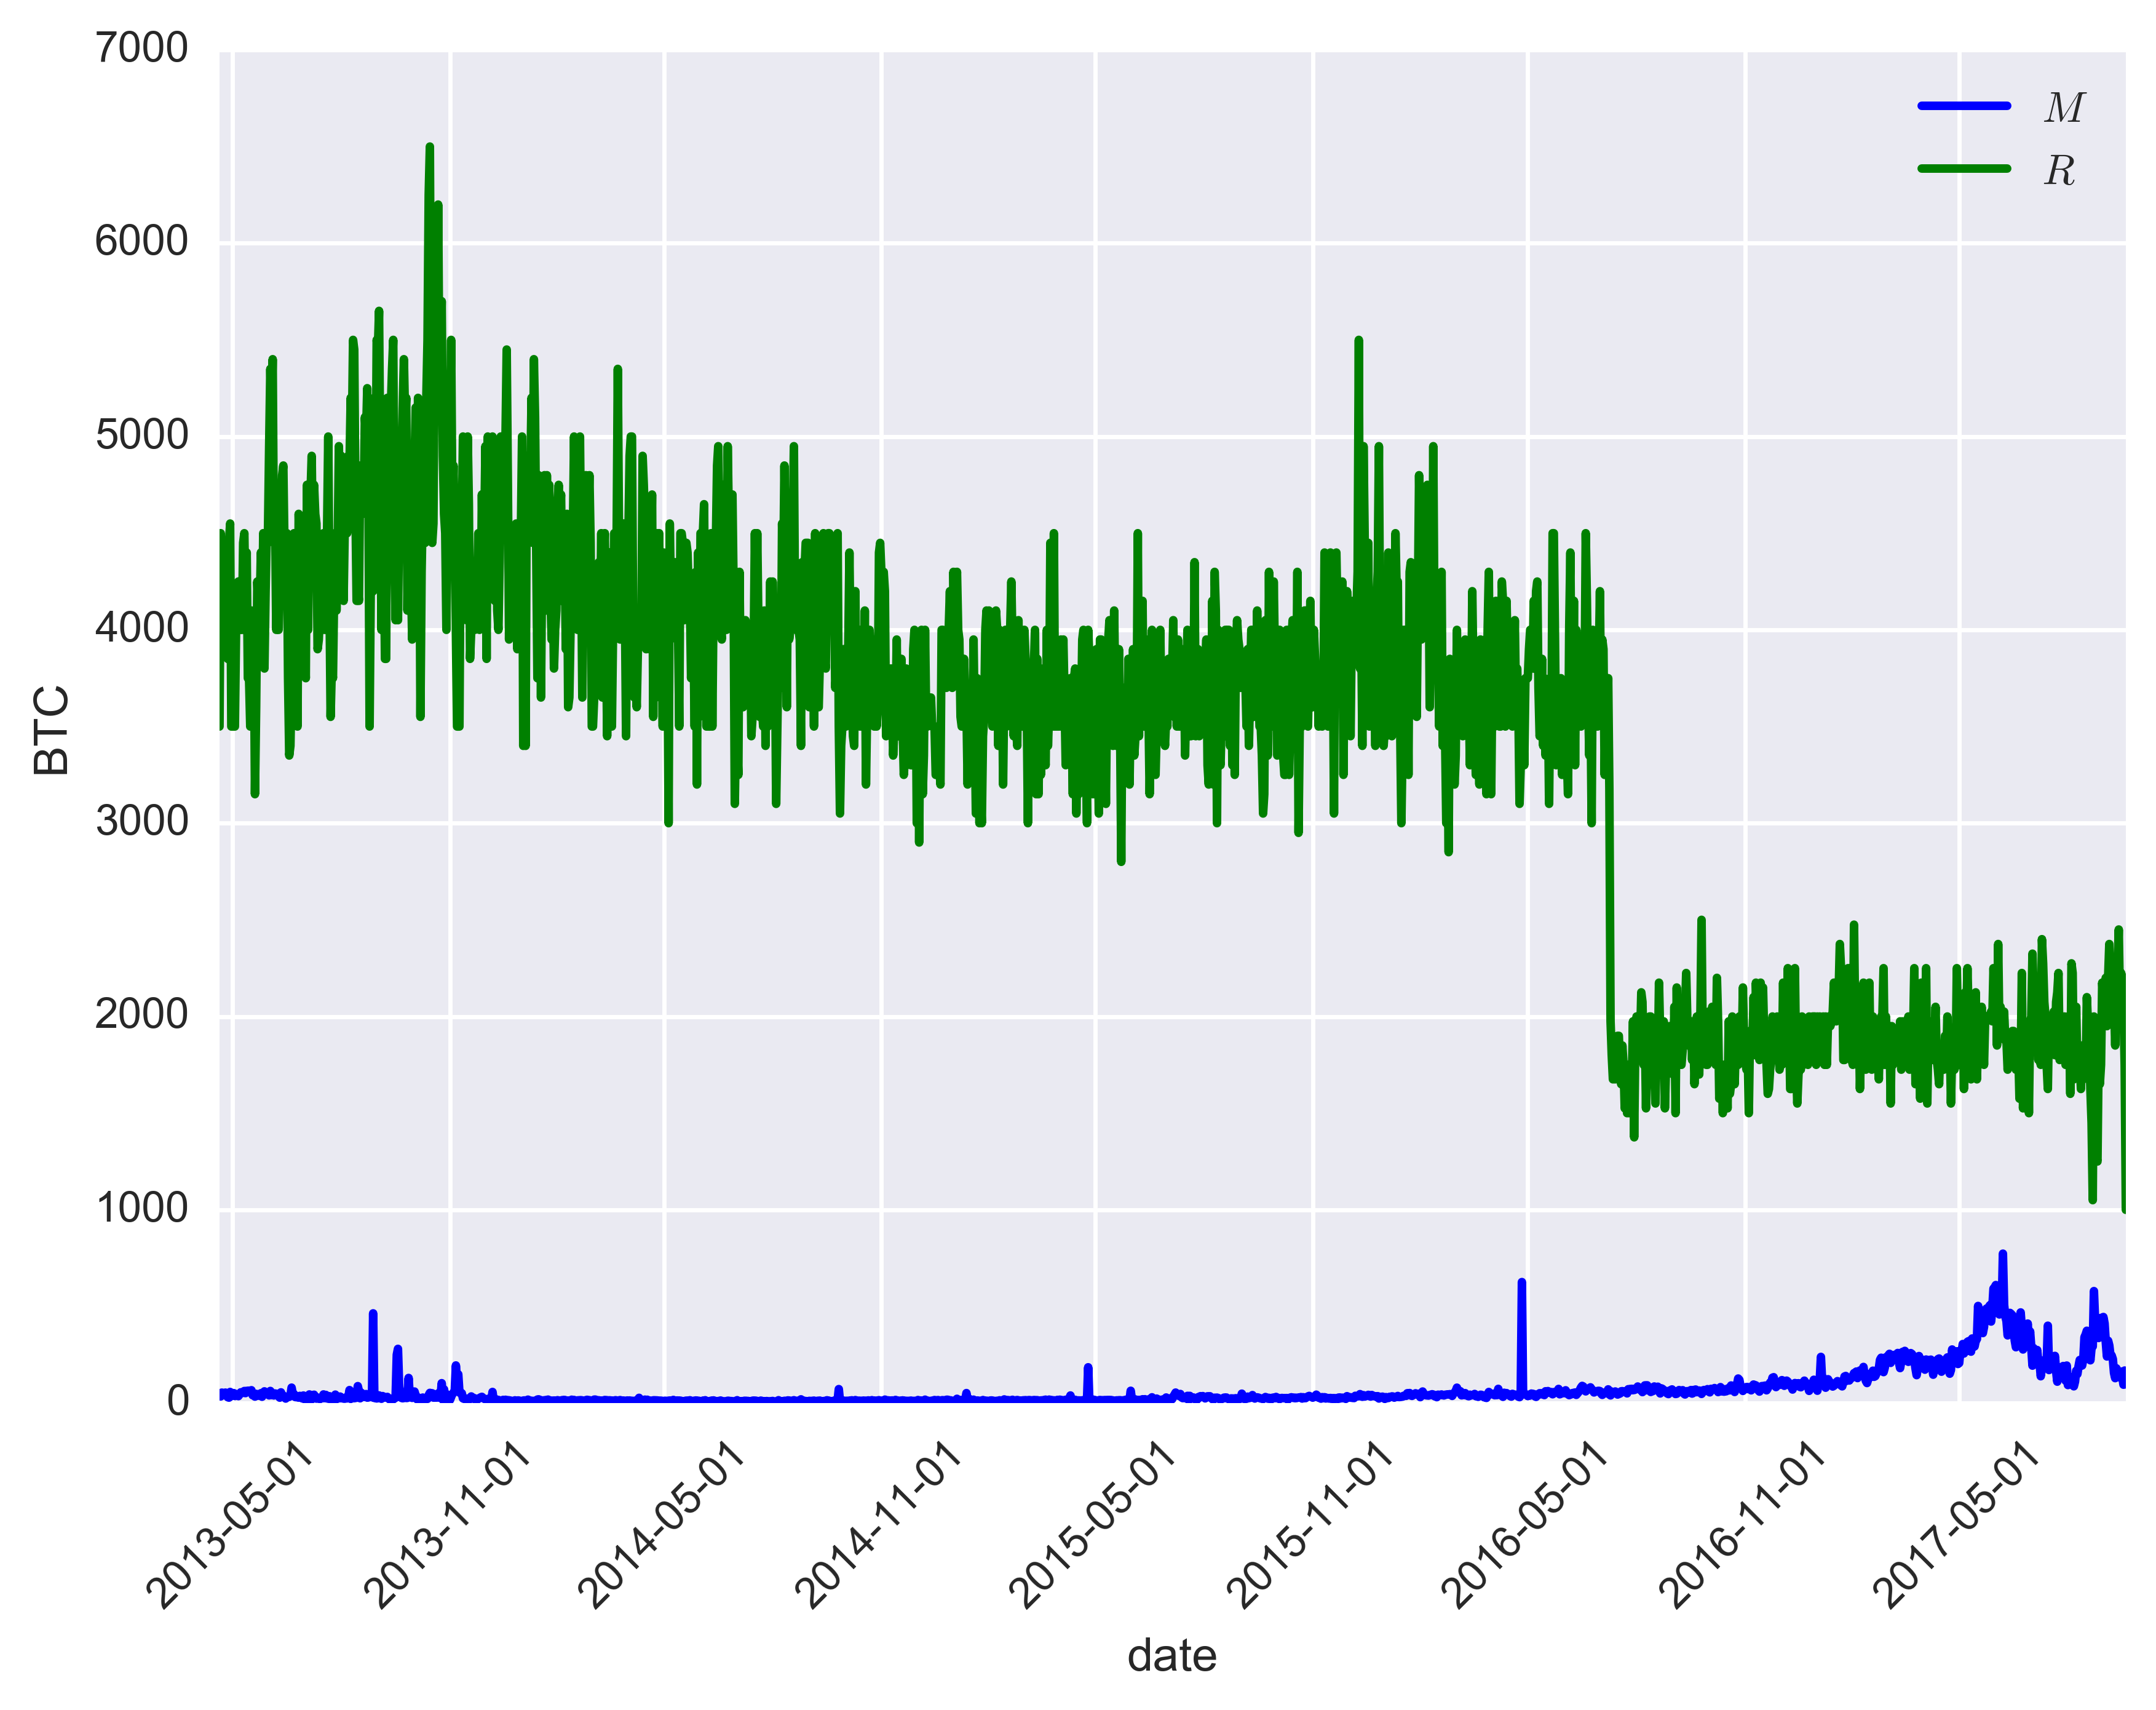
\includegraphics[width=1\textwidth]{img/reward_fee}
	\caption{Miners revenue $\langle V \rangle$ divided in block reward $R$ and sum
		of all $t_f$s in a block, $M$, analyzed between $2013$ and $2015$. Data are
	represented daily, and the $R$ and $M$ values are sums of every specific day.}
	\label{fig:reward_fee}
\end{figure}
If back in $2009$-$2013$ the block revenue was
poorly influenced by user's fees and it relied more
on the reward $R$, we can see instead
in Figure~\ref{fig:reward_fee}, that $R$ is decreasing
while the fees are getting higher, and we expect 
$M$ to overcome $R$ by $2020$ when the
reward is halved again at $6.25$\,\bitcoinA.
We have seen that the block profit $\langle \Pi \rangle$
is highly influenced by users' fees $t_f$,
unfortunately, more miners will request for fee,
more users are discouraged to pay with Bitcoin.
Furthermore we noticed a strong link between
the halving of $R$ in mid $2016$ and the increment of $t_f$.
Because of that we analyzed transaction fees
offered by users to see how they are influenced
in paying more or less \bitcoinA~to the miners during
they years.

\subsubsection{Miner Profit Function}
\label{sec:minerprofitfunction}
To have a mathematical idea of what is happening
between miner's profit and creation time,
we define $f^{2}_{\langle \Pi \rangle}$ as the
\emph{Miner Profit Function}, and represents it in Equation~\ref{eq:miner_profit},
which is inferred after our analysis on almost
twenty-five thousand blocks, considering a single
miner using AntMiner~S$9$, and having $\mathcal{T}$
in minutes as input.
\begin{equation}
\label{eq:miner_profit}
f^{2}_{\langle \Pi \rangle}(\mathcal{T}) = - \frac{1.896}{10^8} x^2 + \frac{5.977}{10^7} x + \frac{3.831}{10^5} \mbox{ }\begin{cases} \mbox{ with } 0 \leq \mathcal{T} < 80 \end{cases}
\end{equation}
%TODO: MAE: 1.1916861568e-05 for f39
%TODO MAE: 1.26572248346e-05 for f2
To optimize the profit $\langle \Pi \rangle$, according
to $f^{2}_{\langle \Pi \rangle}$, the
difficulty should never be increased in a way to
have a creation time $\mathcal{T} >> 20$\,minutes otherwise
miners have a loss in their profit,
and for miner's sake, should be even better to slightly
decrease $\mathcal{T}$ according to avoid
useless computation that leads to a higher cost and waste
of electricity.
We also generate, to have a more accurate trend, $f_{\langle \Pi \rangle}^{39}$,
which is also shown in Figure~\ref{fig:profit_creation_time} but
not mathematically represented, being a $39$ degrees polynomial.
We could use this trend though to assume that the real
profit occurs between $3$ and $8$ minutes,
while having less or more creation time the
$\langle \Pi \rangle$ will not be optimized.

\subsection{Users' Benefits}
\label{sec:userbenefits}
In order to make assumptions and conclusions on how
users should use their fee to optimize their bandwidth in
the system, we first analyze how the $t_f$ changed during
time. Figure~\ref{fig:txs_fee_distribution}, shows the numerical
attribute $t_f$ divided into categories and
represented in percentage for each category.
We can notice that, after the first half of $2016$,
fees between $0$\,\bitcoinA~and $0.0002$\,\bitcoinA~almost disappeared
from the system, and considering that the Bitcoin price raised
from less than $1000$\,\$ to more than $5000$\,\$ between
mid $2016$ and second half of $2017$, this results to be
as a huge increment on the fees paid to miners, especially if
we consider that, if we compare the Bitcoin price and the fee paid
in \gls{usd}, we see a substantial co-movement which indicates
that \gls{btc} is the dominant unit of account when deciding about
the fee offers. Is possible also to see this increment in
Figure~\ref{fig:reward_fee},
indeed the total $t_f$ paid to miners almost reaches
$1000$\,\bitcoinA~per day $2017$.
We can also see that we had
higher fees early in $2013$, but at the time the \gls{usd}
price for Bitcoin was less than $120$\,\$ so respectively the fees
were much lower. We believe that, events happening
on the Bitcoin blockchain might influence fee, tolls and
the way blocks choose transactions, and to confirm
our assumptions we see that the biggest
increment in $t_f$ was in late $2016$, which coincides
with the halving of $R$ and the blocks saturation.
%TODO: Define when is convenient for users to pay fee for bandwidth
%TODO: Proved that from 2013 to 2017 the $t_l$ is more dependent from the $t_f$ 
\begin{figure}[h]
	\centering
	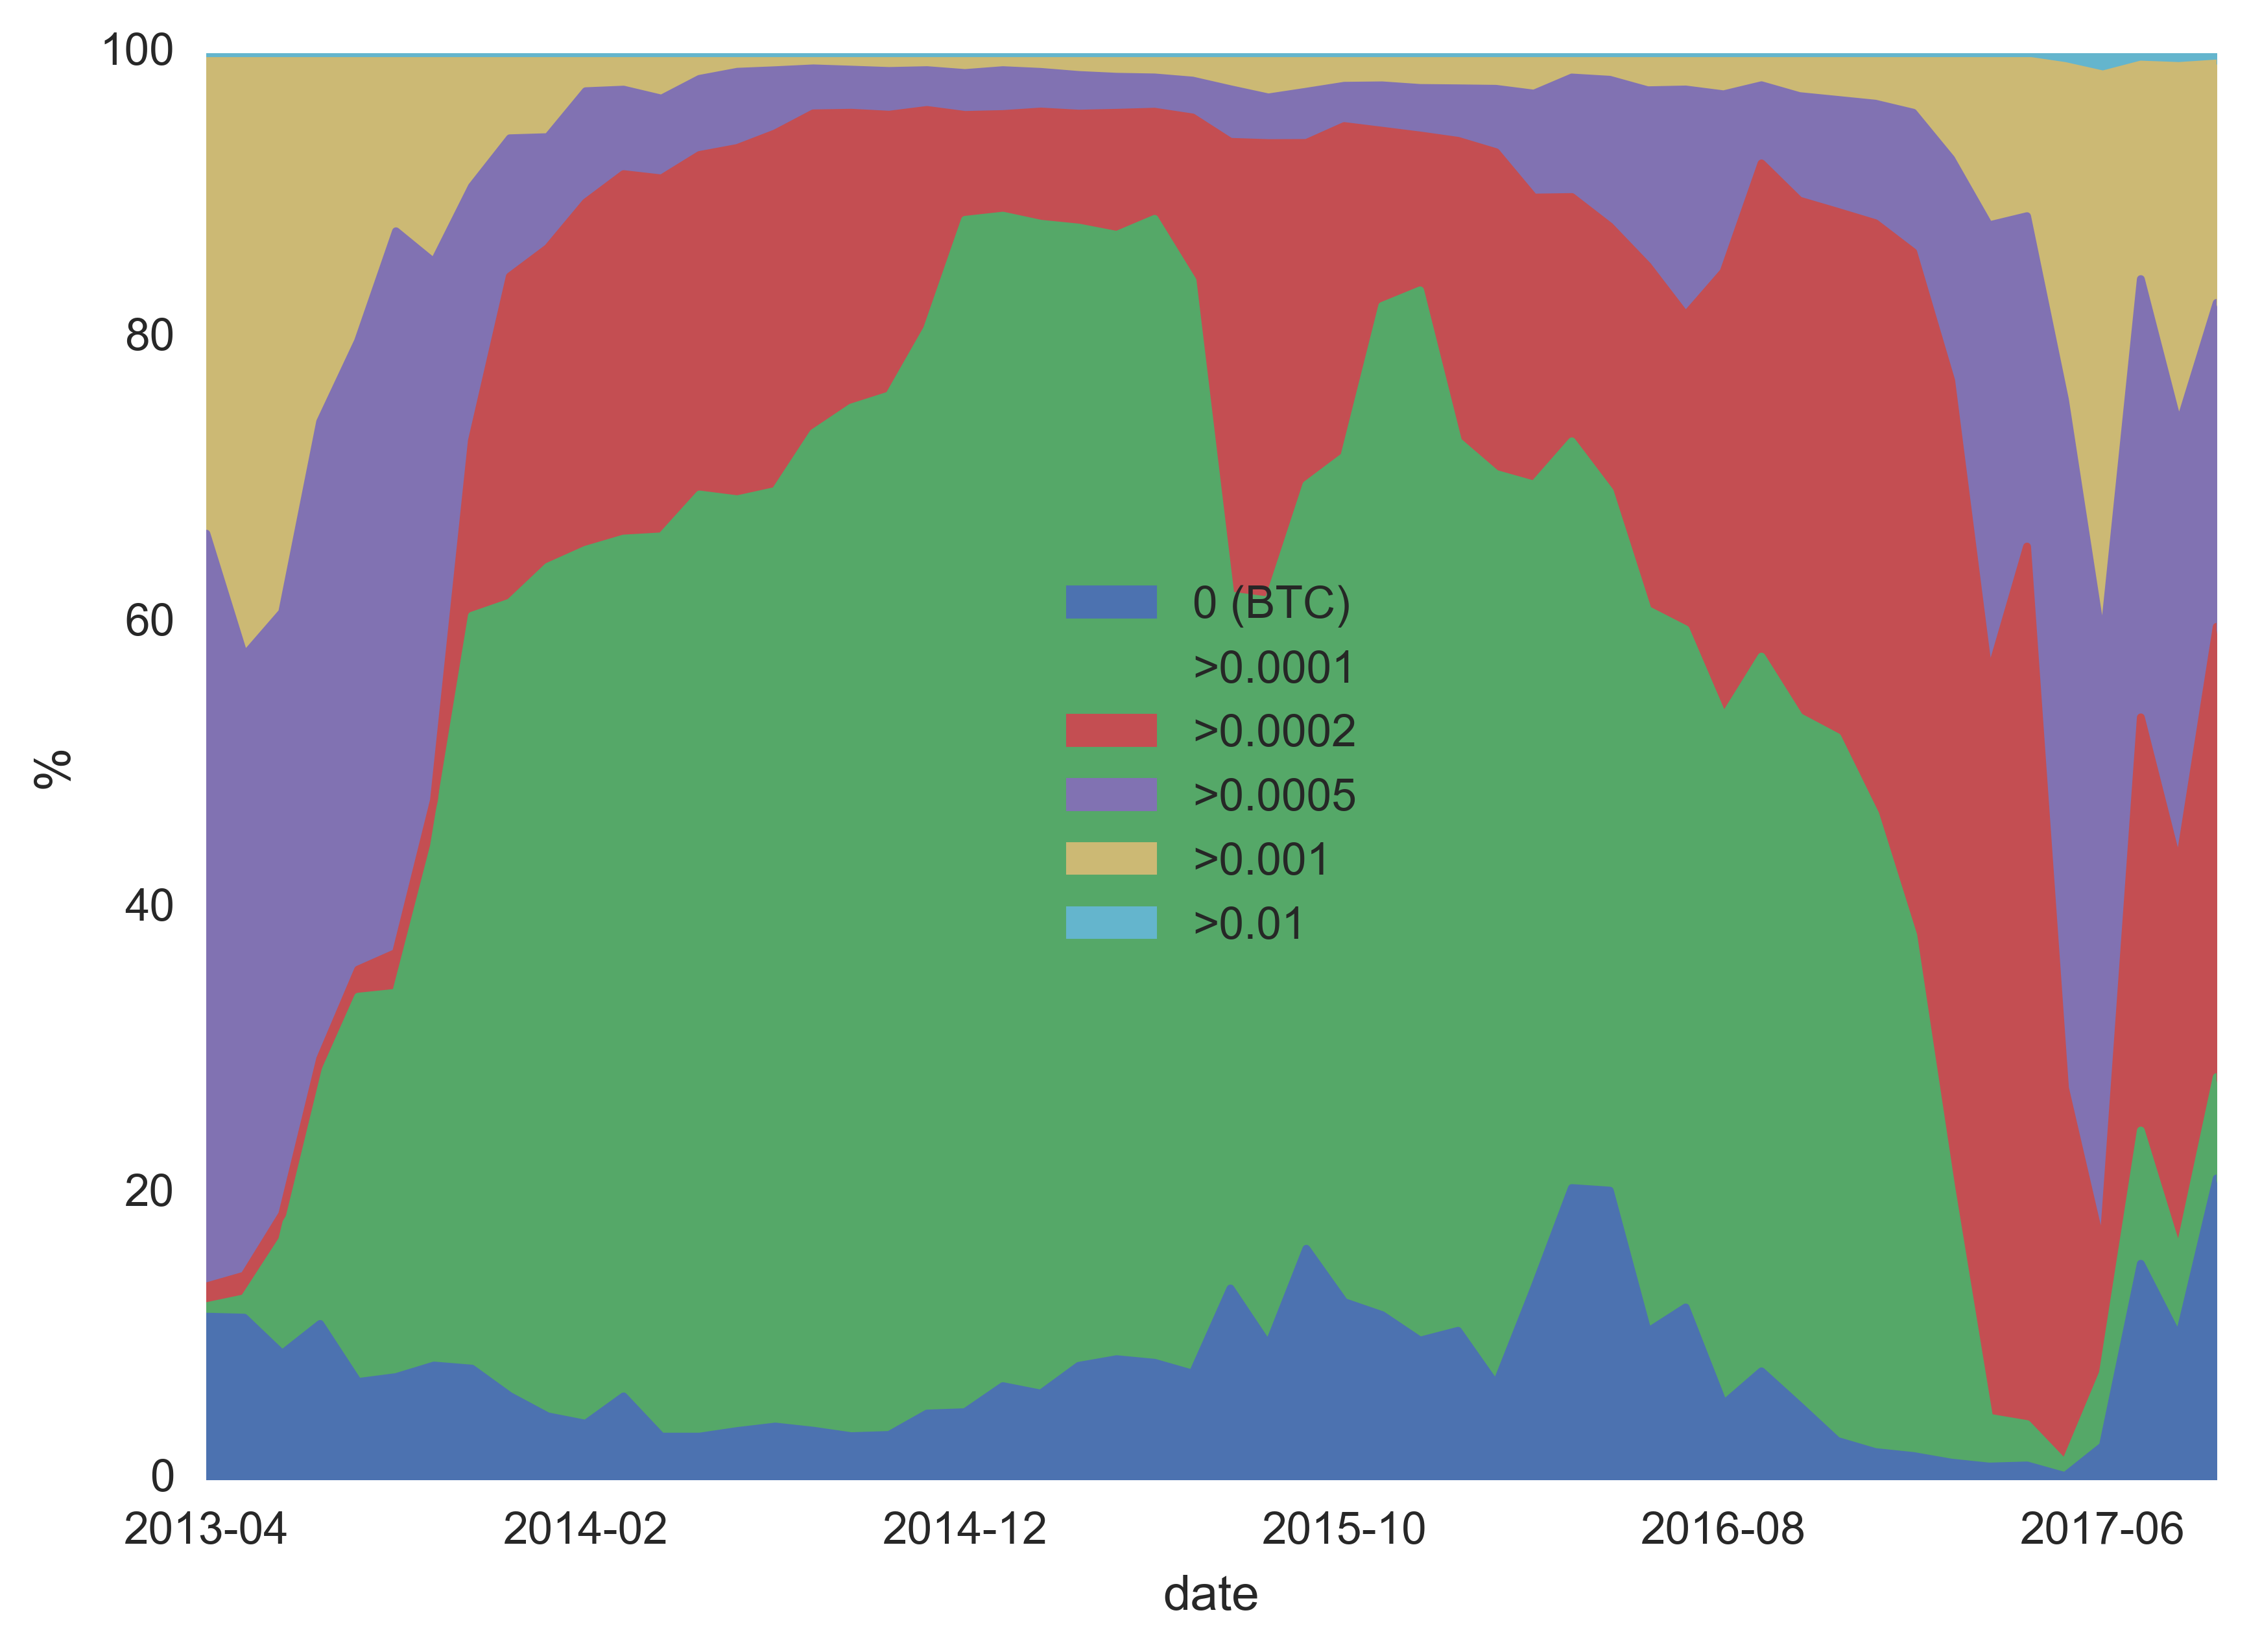
\includegraphics[width=1\textwidth]{img/txs_fee_distribution}
	\caption{Transaction fee ($t_f$) distribution during the years from
		$2013$ until $2017$.}
	\label{fig:txs_fee_distribution}
\end{figure}
To see how miners change their behavior according to
events happening on the Bitcoin system we study the fee density
$\rho$, defined in Equation~\ref{eq:feedensity} and displayed in
Figure~\ref{fig:txs_feedensity_distribution}.
Fee density and fee are directly connected,
since the transaction size $t_q$ has an average of $500$\,bytes,
but at the end of $2017$, even if we have some fees with
$<0.0001$\,\bitcoinA, we almost never
have transactions with a $\rho = 0$,
which means that recently, miners might have changed
from having constraints on fees to having constraints
on fee density.
\begin{figure}[h]
	\centering
	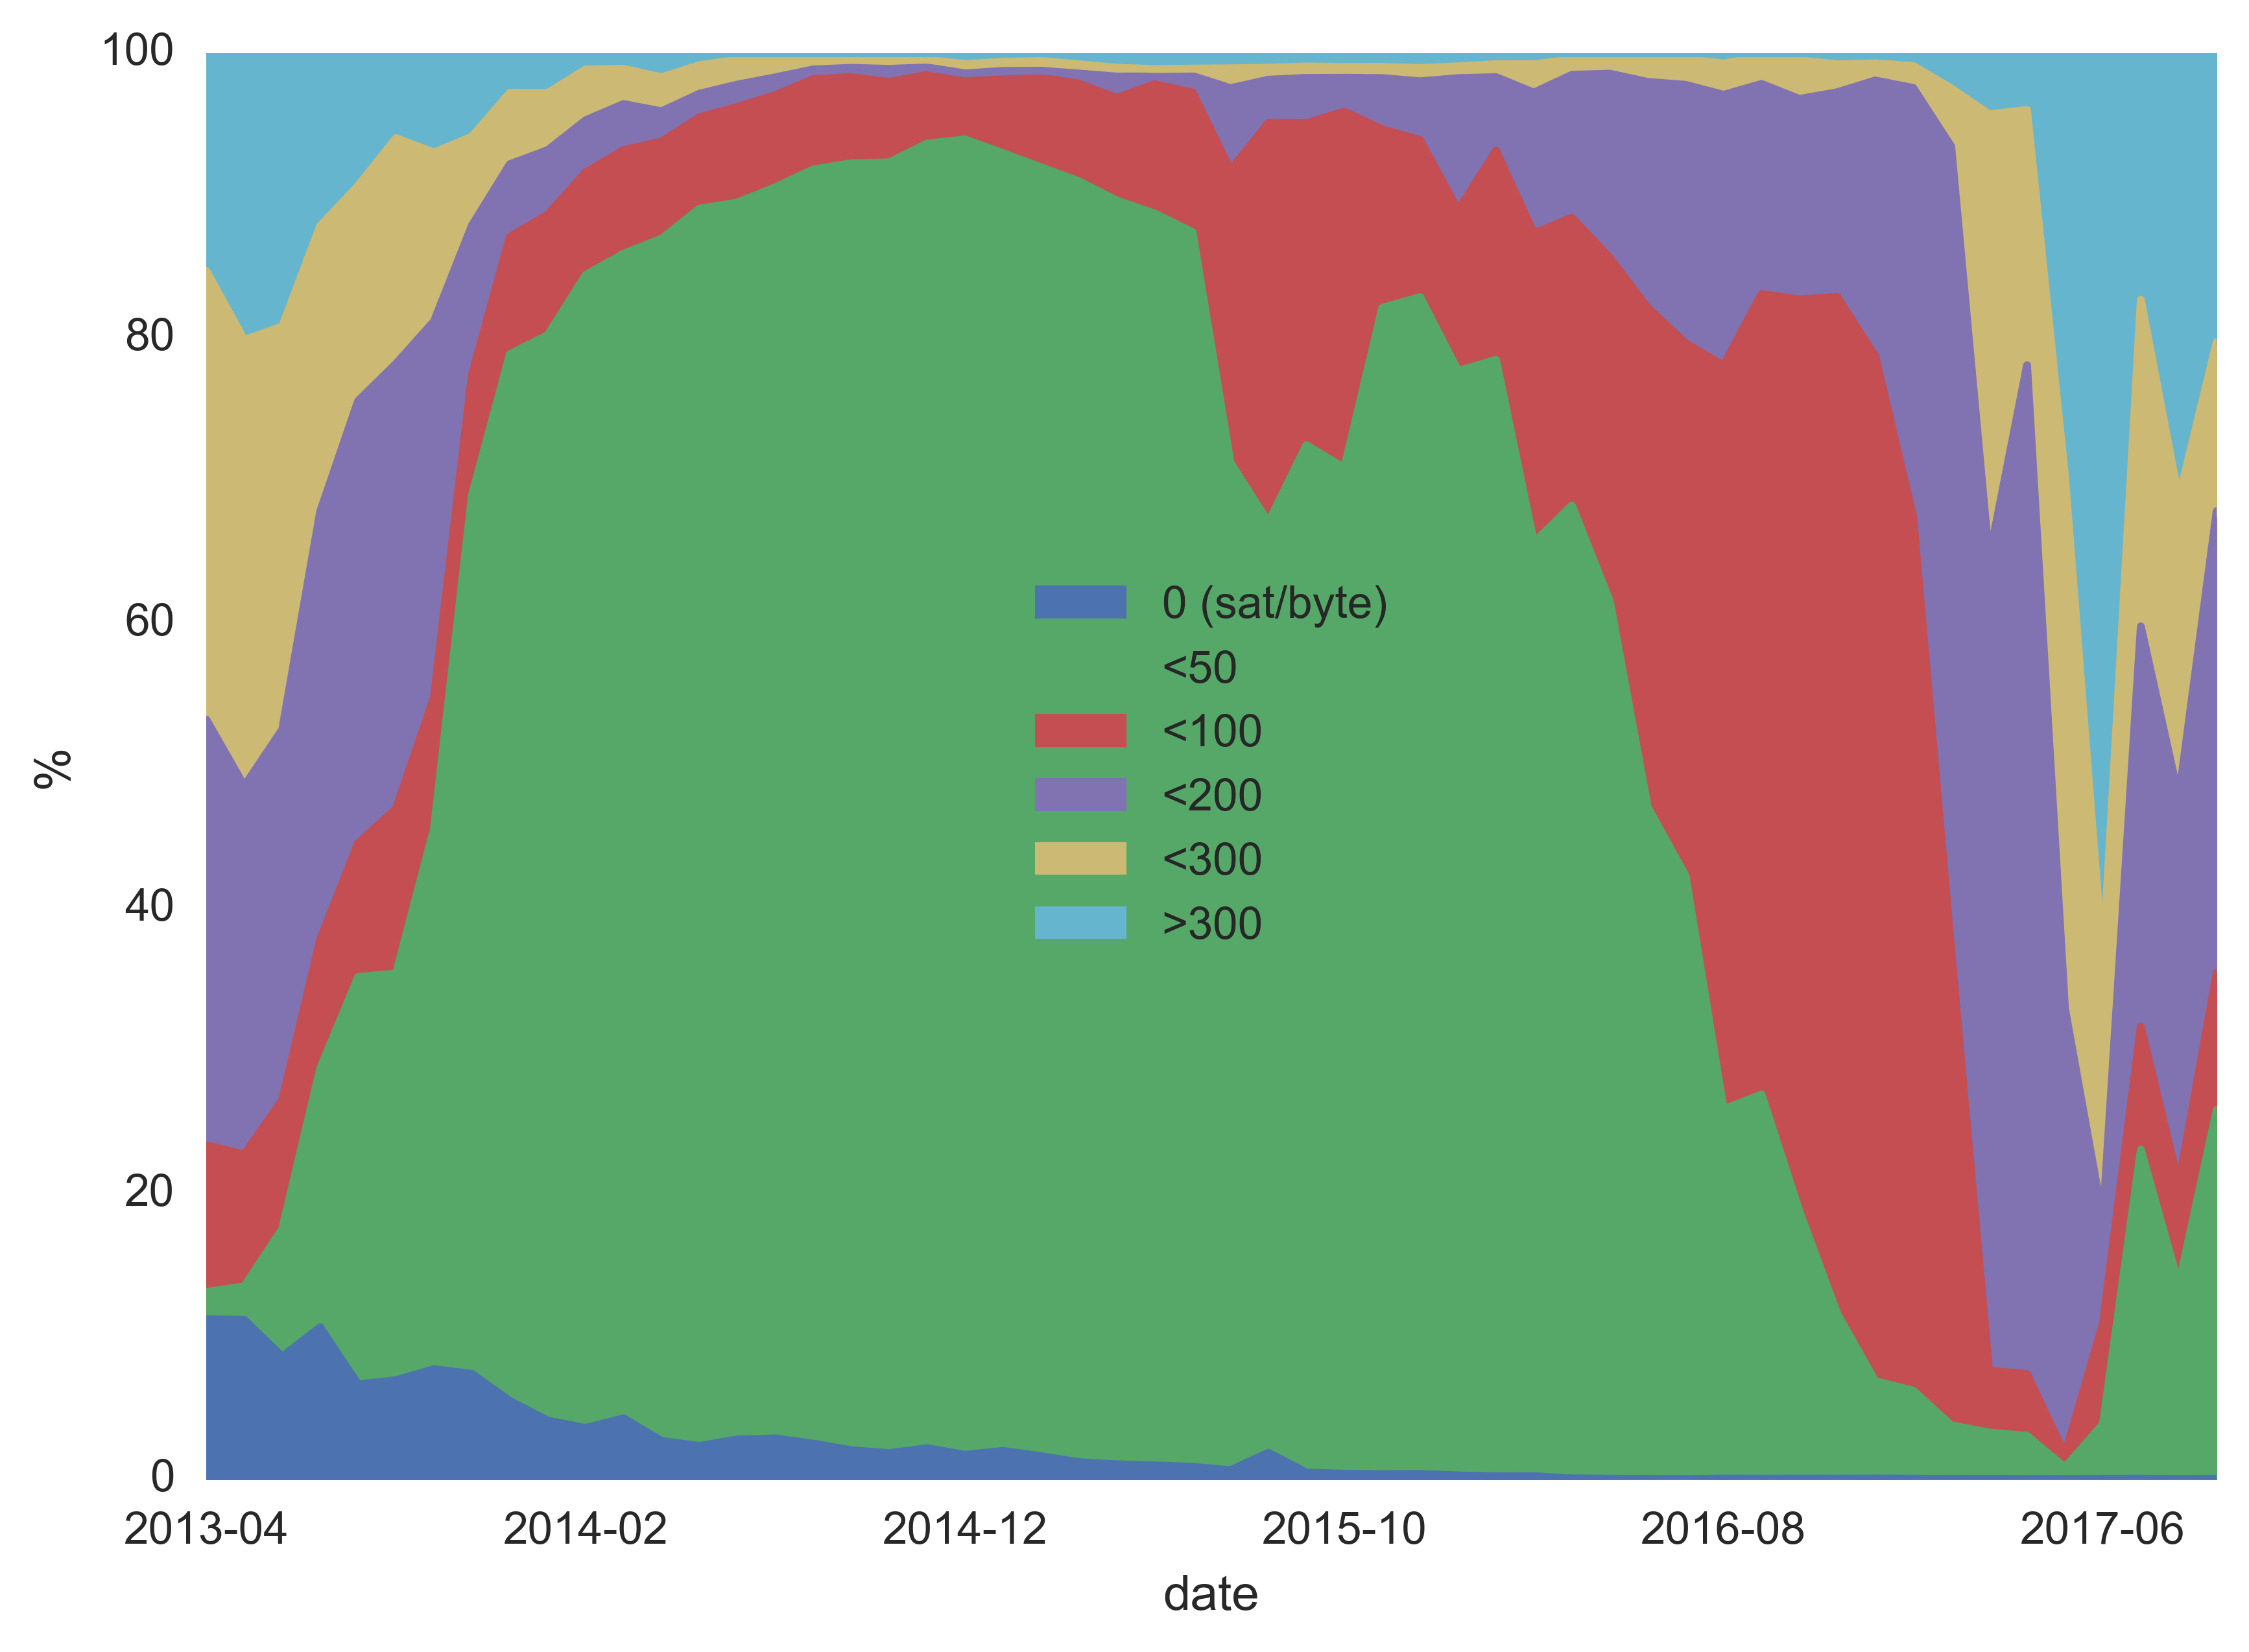
\includegraphics[width=1\textwidth]{img/txs_feedensity_distribution}
	\caption{Fee density ($\rho$) distribution during the years from
		$2013$ until $2017$.}
	\label{fig:txs_feedensity_distribution}
\end{figure}
This drastic change in $t_f$ and $\rho$
lead us to think that there is another factor which is
influenced by it, and in our assumptions we thought it
was the transaction latency $t_l$. This is the reason why,
we analyzed $t_l$ in function of $t_f$ from $2013$ to
$2017$~(Figure~\ref{fig:fee_latency}) for an overall
trend, and then $t_l$ in function of $t_f$ and $\rho$
for transactions occurred in $2017$ to generate our prediction
models. As also Figure~\ref{fig:fee_latency} shows, is not
good to invest in so much high fees, since after a certain
threshold, the latency would be even higher. With our
models we want to define these thresholds and give users
some ideas on how they might invest wisely their money,
according to optimize their bandwidth.
With data regarding transactions evaluated in $2017$
we generate two models, \emph{Fee Density - Latency Function},
$f_{t_l}(\rho)$, represented in Equation~\ref{eq:feedensity_latency_function},
and \emph{Latency Function}, $f_{t_l}(t_f)$
presented in Equation~\ref{eq:latency_function}.
In Figures~\ref{fig:fee_latency_regression},~\ref{fig:feedensity_latency},
due to our interpolation function's boundaries, we
show two different degrees of
polynomial interpolation, $f_{t_l}^2$ and $f_{t_l}^{39}$.
The purpose of $f_{t_l}^2$ is to have a general equation
to refer on while talking about fees and latency, while
the $f_{t_l}^{39}$ gives us more strict thresholds about
the trend our data tend to follow, for example in
Figure~\ref{fig:fee_latency} we see that in
$2017$, if you pay more than $0.001$\,\bitcoinA,
you most likely get an increment in your
transaction approval time, and in
Figure~\ref{fig:fee_latency_regression},
$f_{t_l}^{39}$ shows this threshold while $f_{t_l}^2$ does not.
\begin{equation}
\label{eq:latency_function}
f_{t_l}^2 (t_f) = 6248x^2 - 555.8x + 1.42
\end{equation}
%TODO: MAE: 1.75492495754 f2
%TODO: MAE: 1.7475919458 f39
\begin{figure}[h]
	\centering
	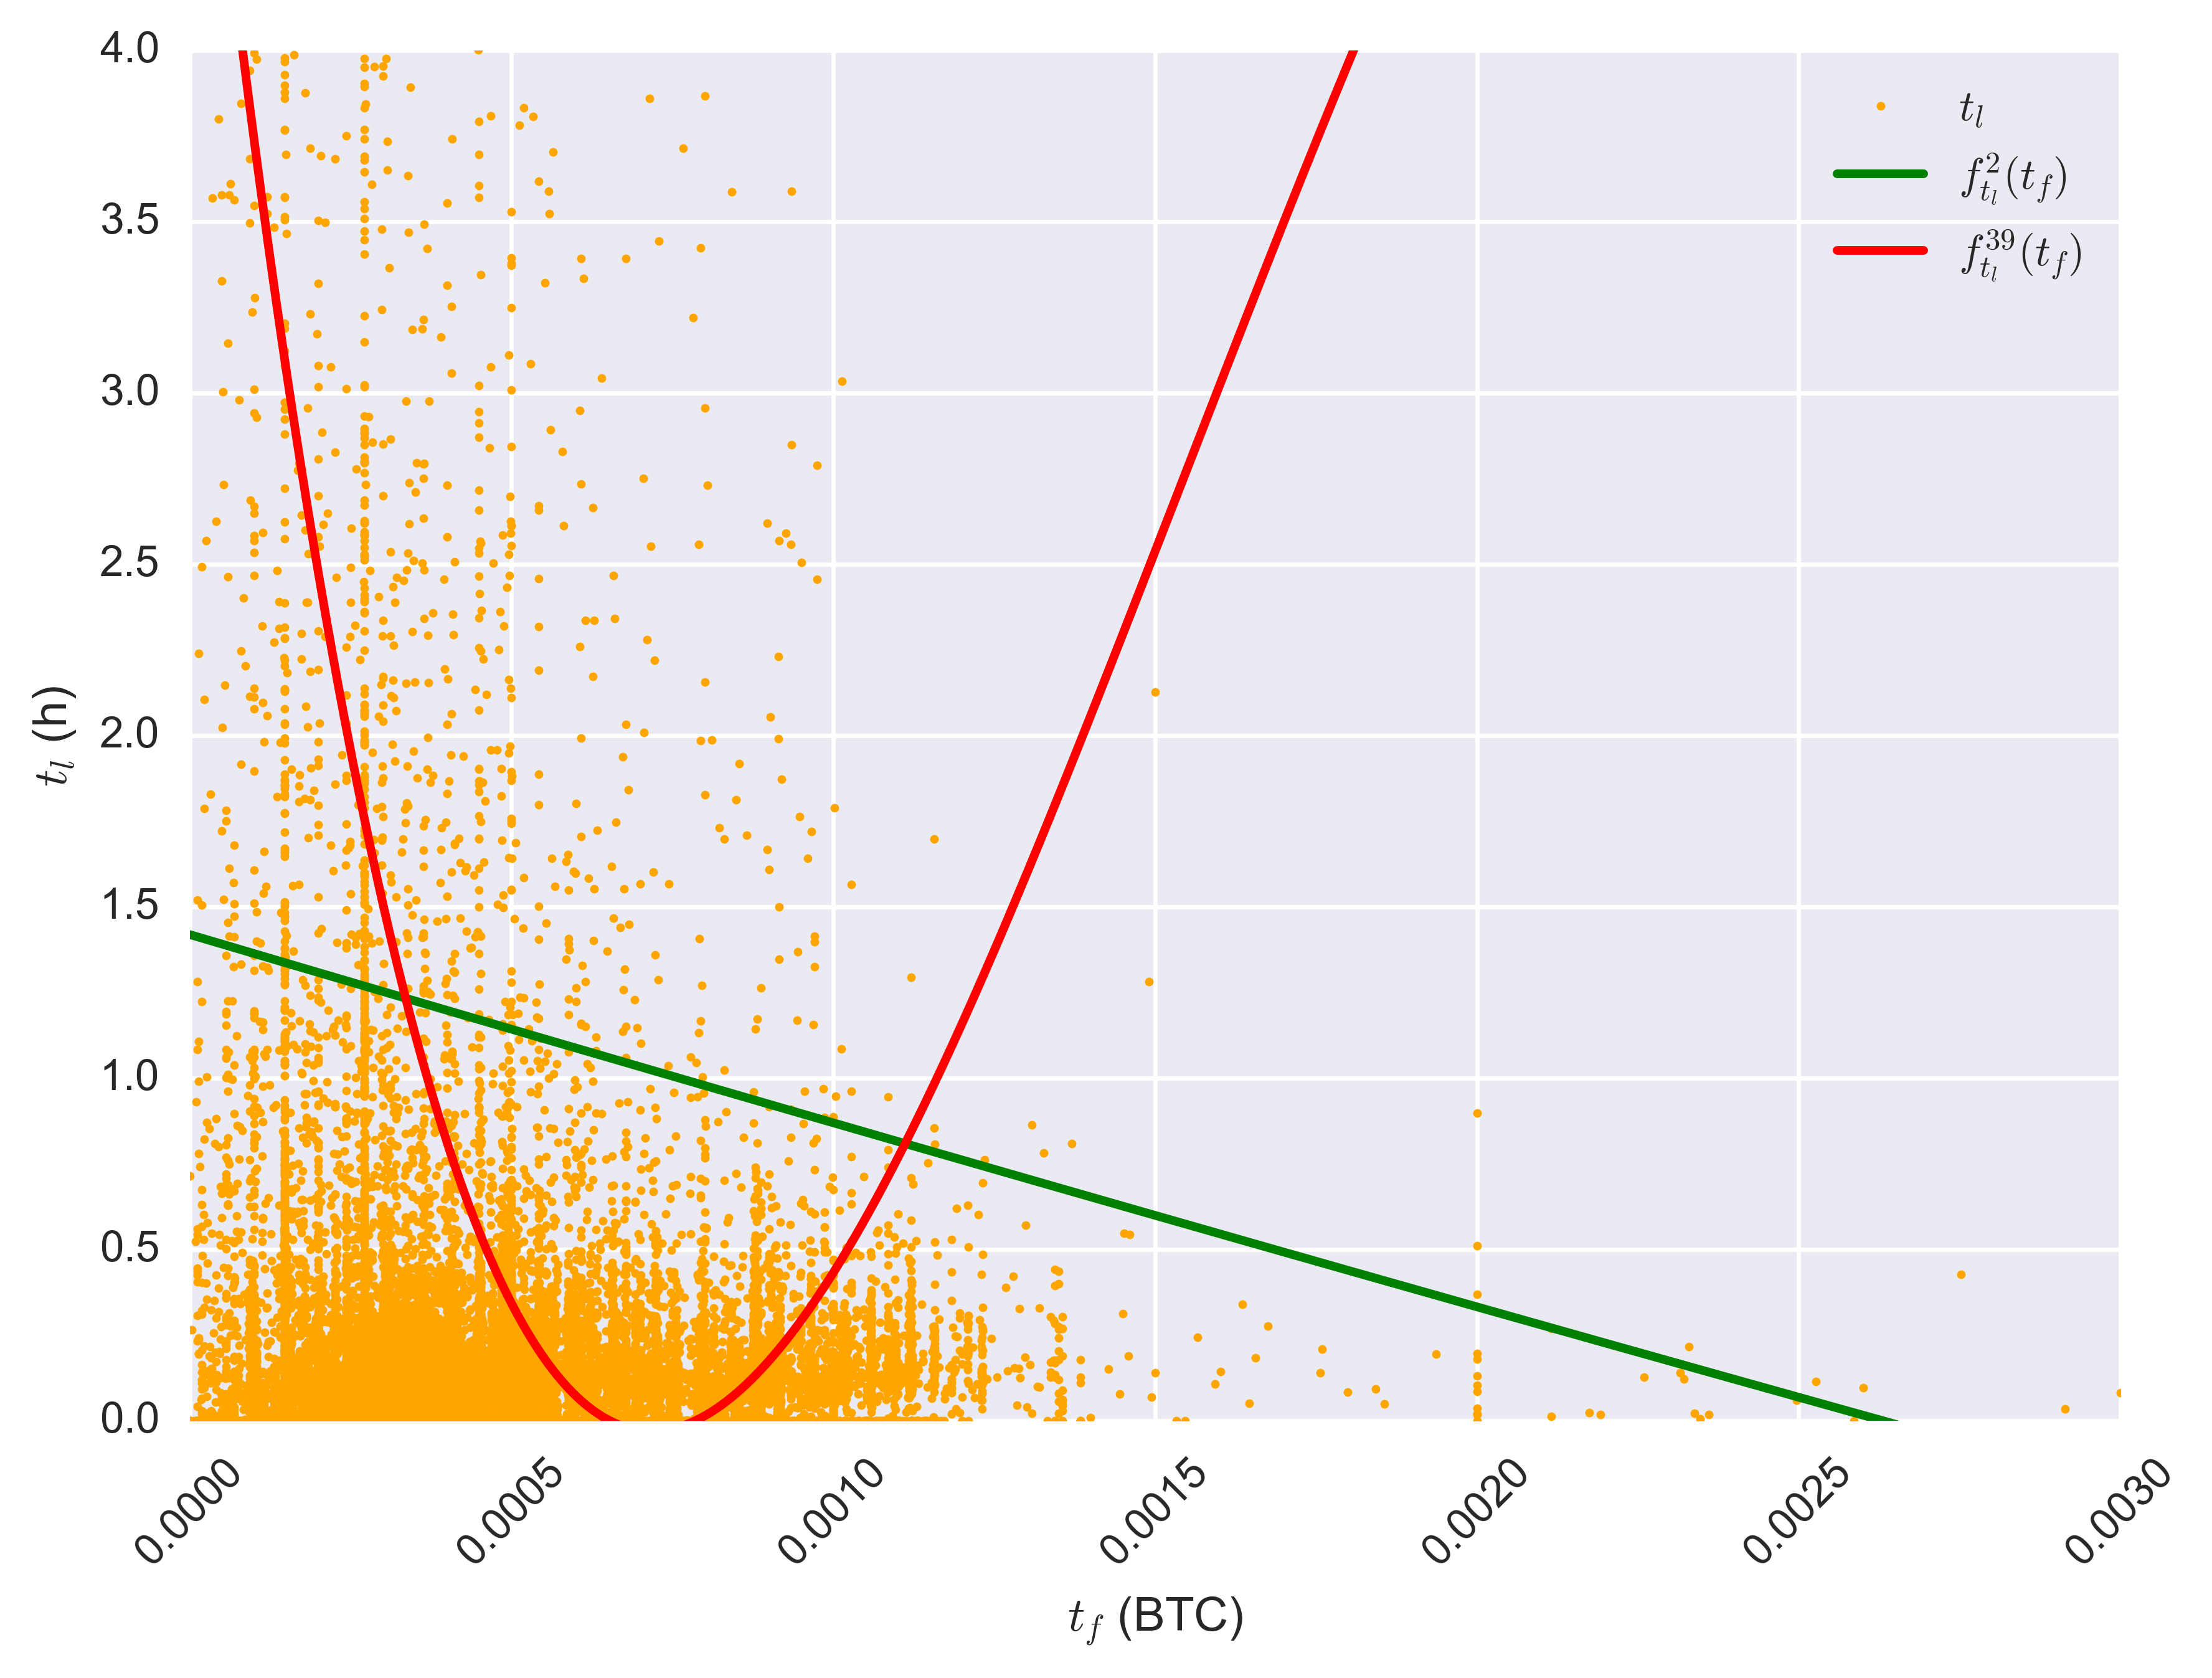
\includegraphics[width=1\textwidth]{img/fee_latency_regression}
	\caption{Interpolation with a $2$ and $39$ degrees polynomial of the relation
		between $t_f$ and $t_l$, for transactions analyzed in $2017$.}
	\label{fig:fee_latency_regression}
\end{figure}
%TODO: MAE: 1.74946761626 f2
%TODO: MAE: 1.83650505922 f39
\begin{equation}
\label{eq:feedensity_latency_function}
f_{t_l}^2 (\rho) = \frac{5.416}{10^{8}} x^2 - \frac{2.215}{10^{3}}x + 1.598
\end{equation}
\begin{figure}[h]
	\centering
	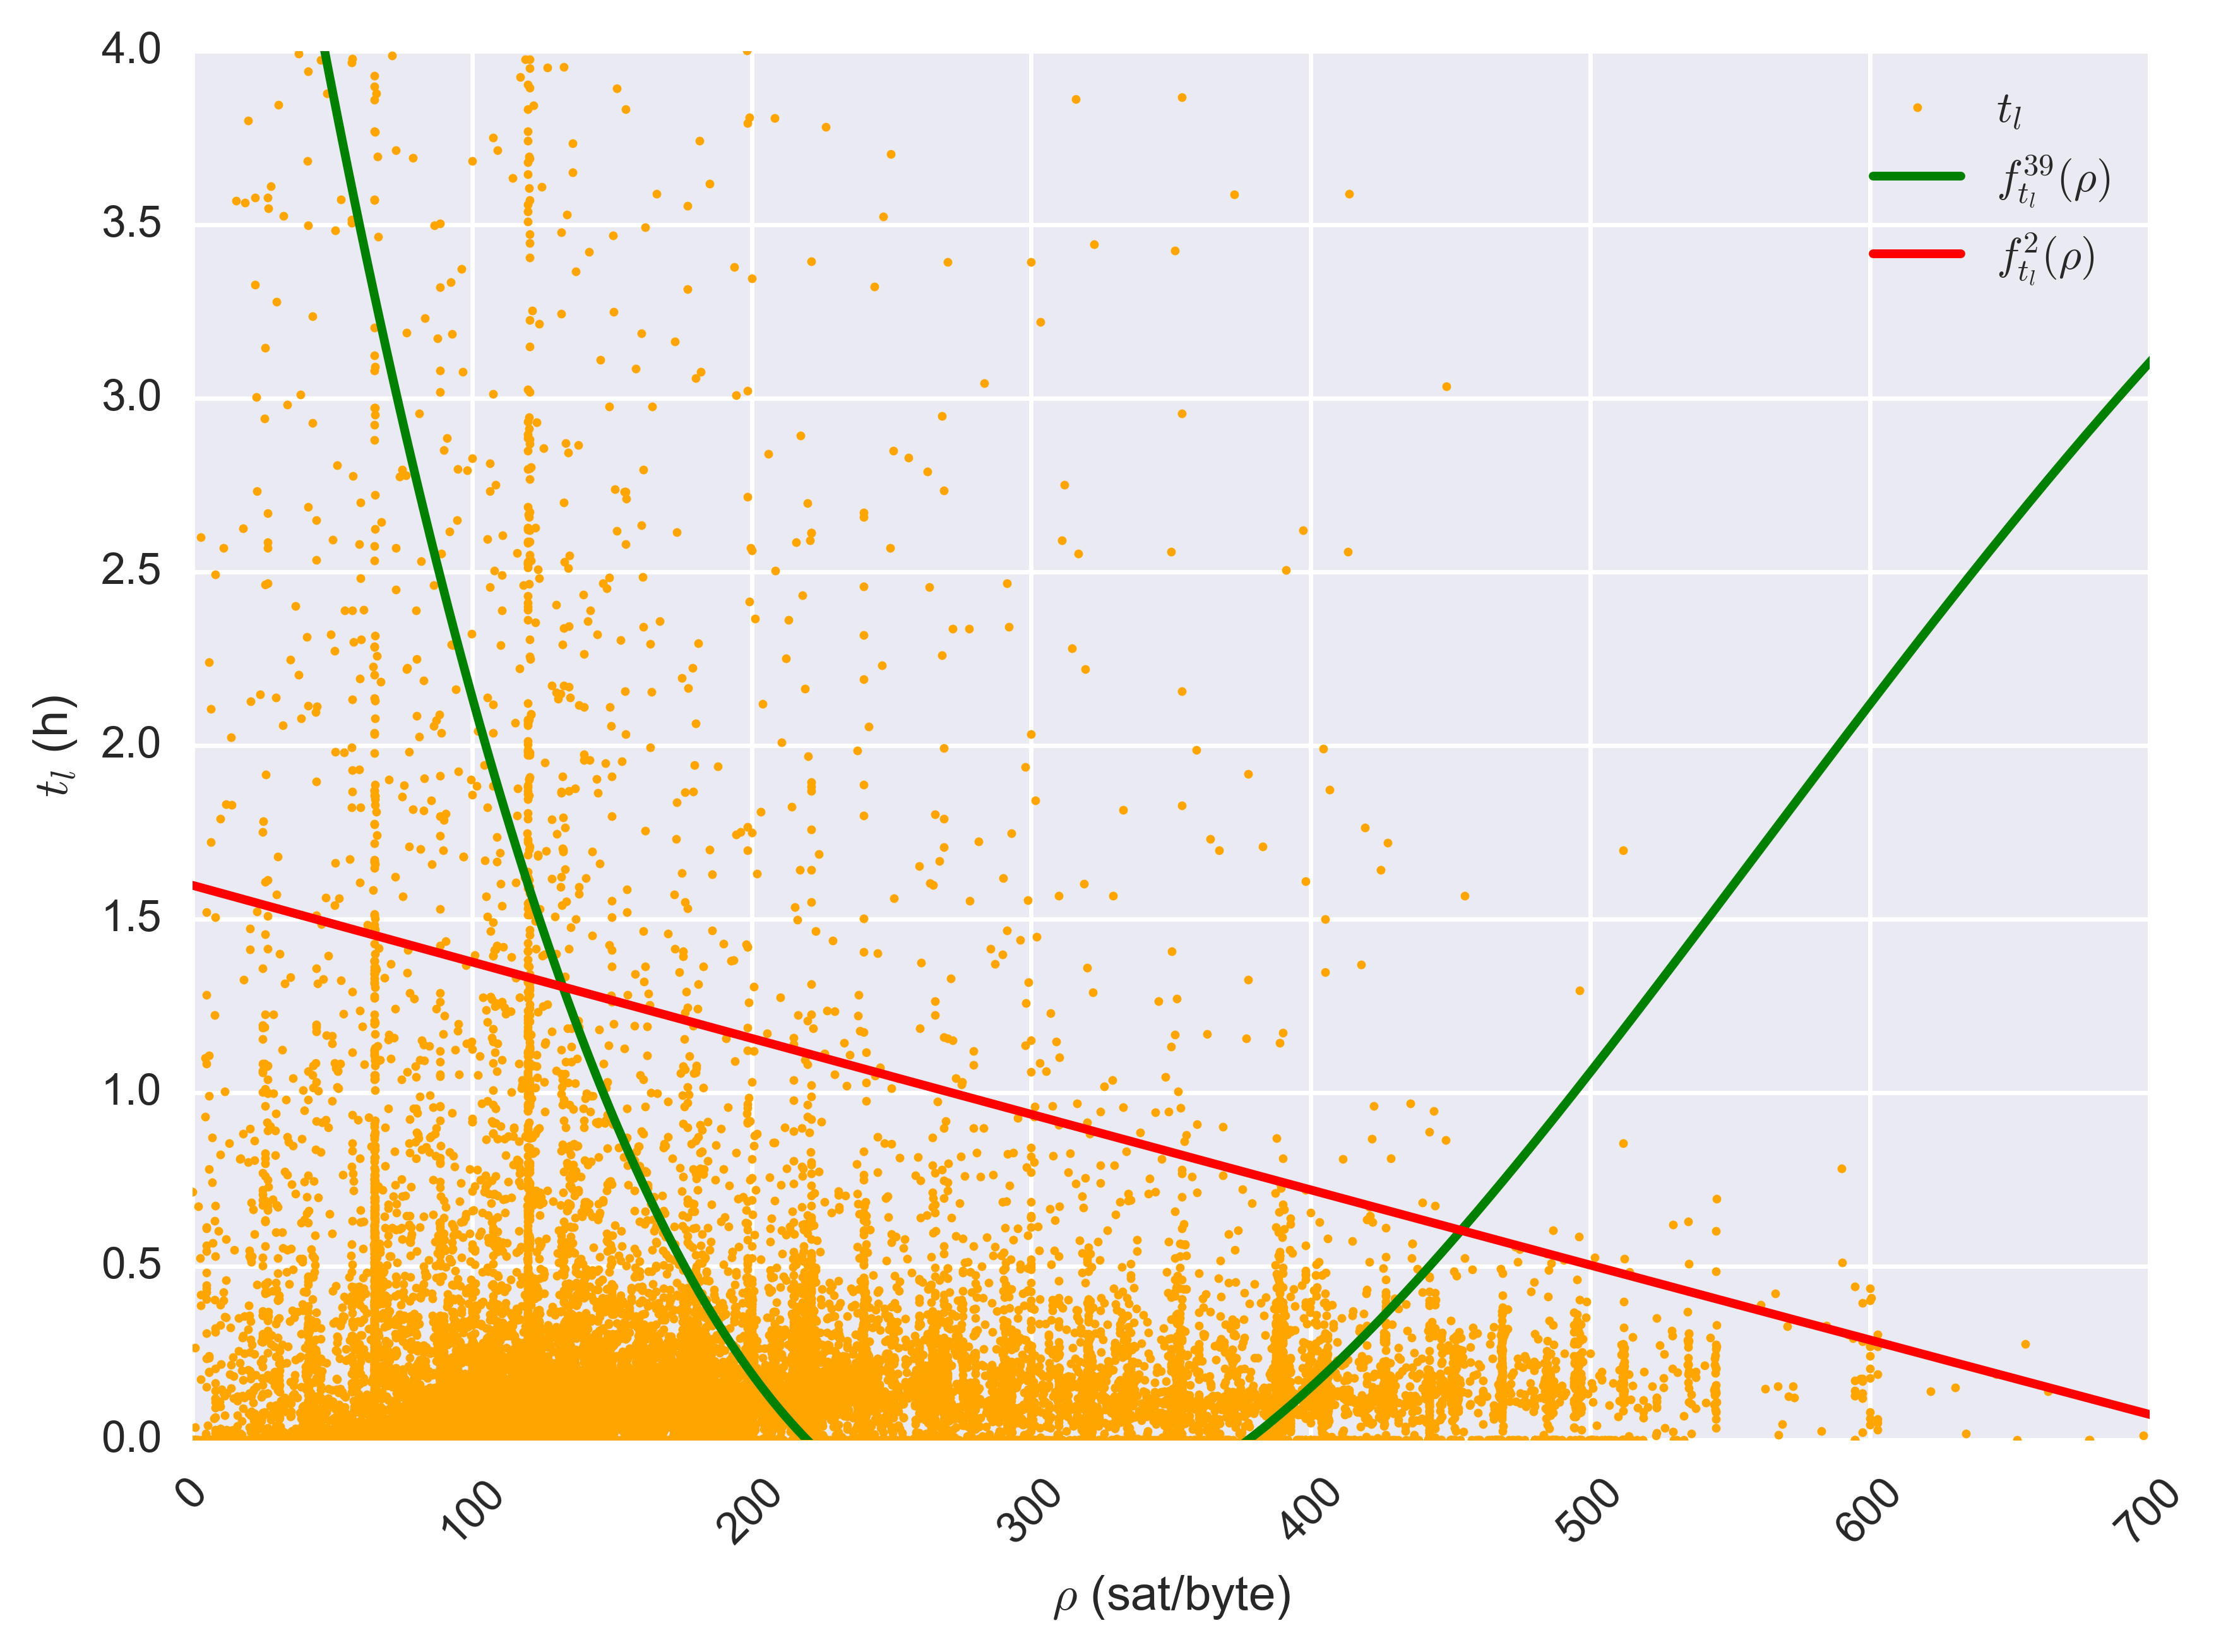
\includegraphics[width=1\textwidth]{img/feedensity_latency}
	\caption{Interpolation with a $2$ and $39$ degrees polynomial of the relation
		between $\rho$ and $t_l$, for transactions analyzed in $2017$.}
	\label{fig:feedensity_latency}
\end{figure}
We can define in that way the thresholds in which our functions
might work and they might be the following:
\[
0 \leq t_f \leq 0.0011,
\]
and
\[
0 \leq \rho \leq 460.
\]
If the $f_{t_l}^2$ function is used to make predictions and
your $t_f$ and $\rho$ are outside this thresholds,
then predictions might not be accurate and plus, you
might be losing more money while getting even an
higher latency. In conclusion, with data collected
for the whole $2017$, we can state that a user
can definitely pay for bandwidth in Bitcoin's
applications but it shouldn't be willing to
offer more than $0.0011$\,\bitcoinA~or
it might waste those money for no reasons.
In addition, if nowadays miners tend to
consider $\rho$ rather than $t_f$, is good
for users to know that an optimal $\rho$ according to
get higher latency would be between $200$
and $300$\,sat/byte.

%TODO: PERCENTAGE OF TRANSACTION FEE
Now if we consider our $t_f$ as a percentage of the
total output $t_{ou}$, where $t_f\% = (t_f \times 100)/t_{ou}$,
also the overall percentage $t_f\%$ had a consistent
increment during the years and from all mining pools,
like Figure~\ref{fig:fee_input_miners} shows, going from
less than $0.05\%$ between $2013$ and $2015$, to
more than $0.2\%$, reaching also $0.3\%$ in $2017$.
Considering now that the Bitcoin price raised from
$1000\$$ to more than $7000\$$ in the last two years,
this increment in the $t_f\%$ results as a huge addition
to the costs for users, and Bitcoin might not be as cheap
as it claims to be.
\begin{figure}[h]
	\centering
	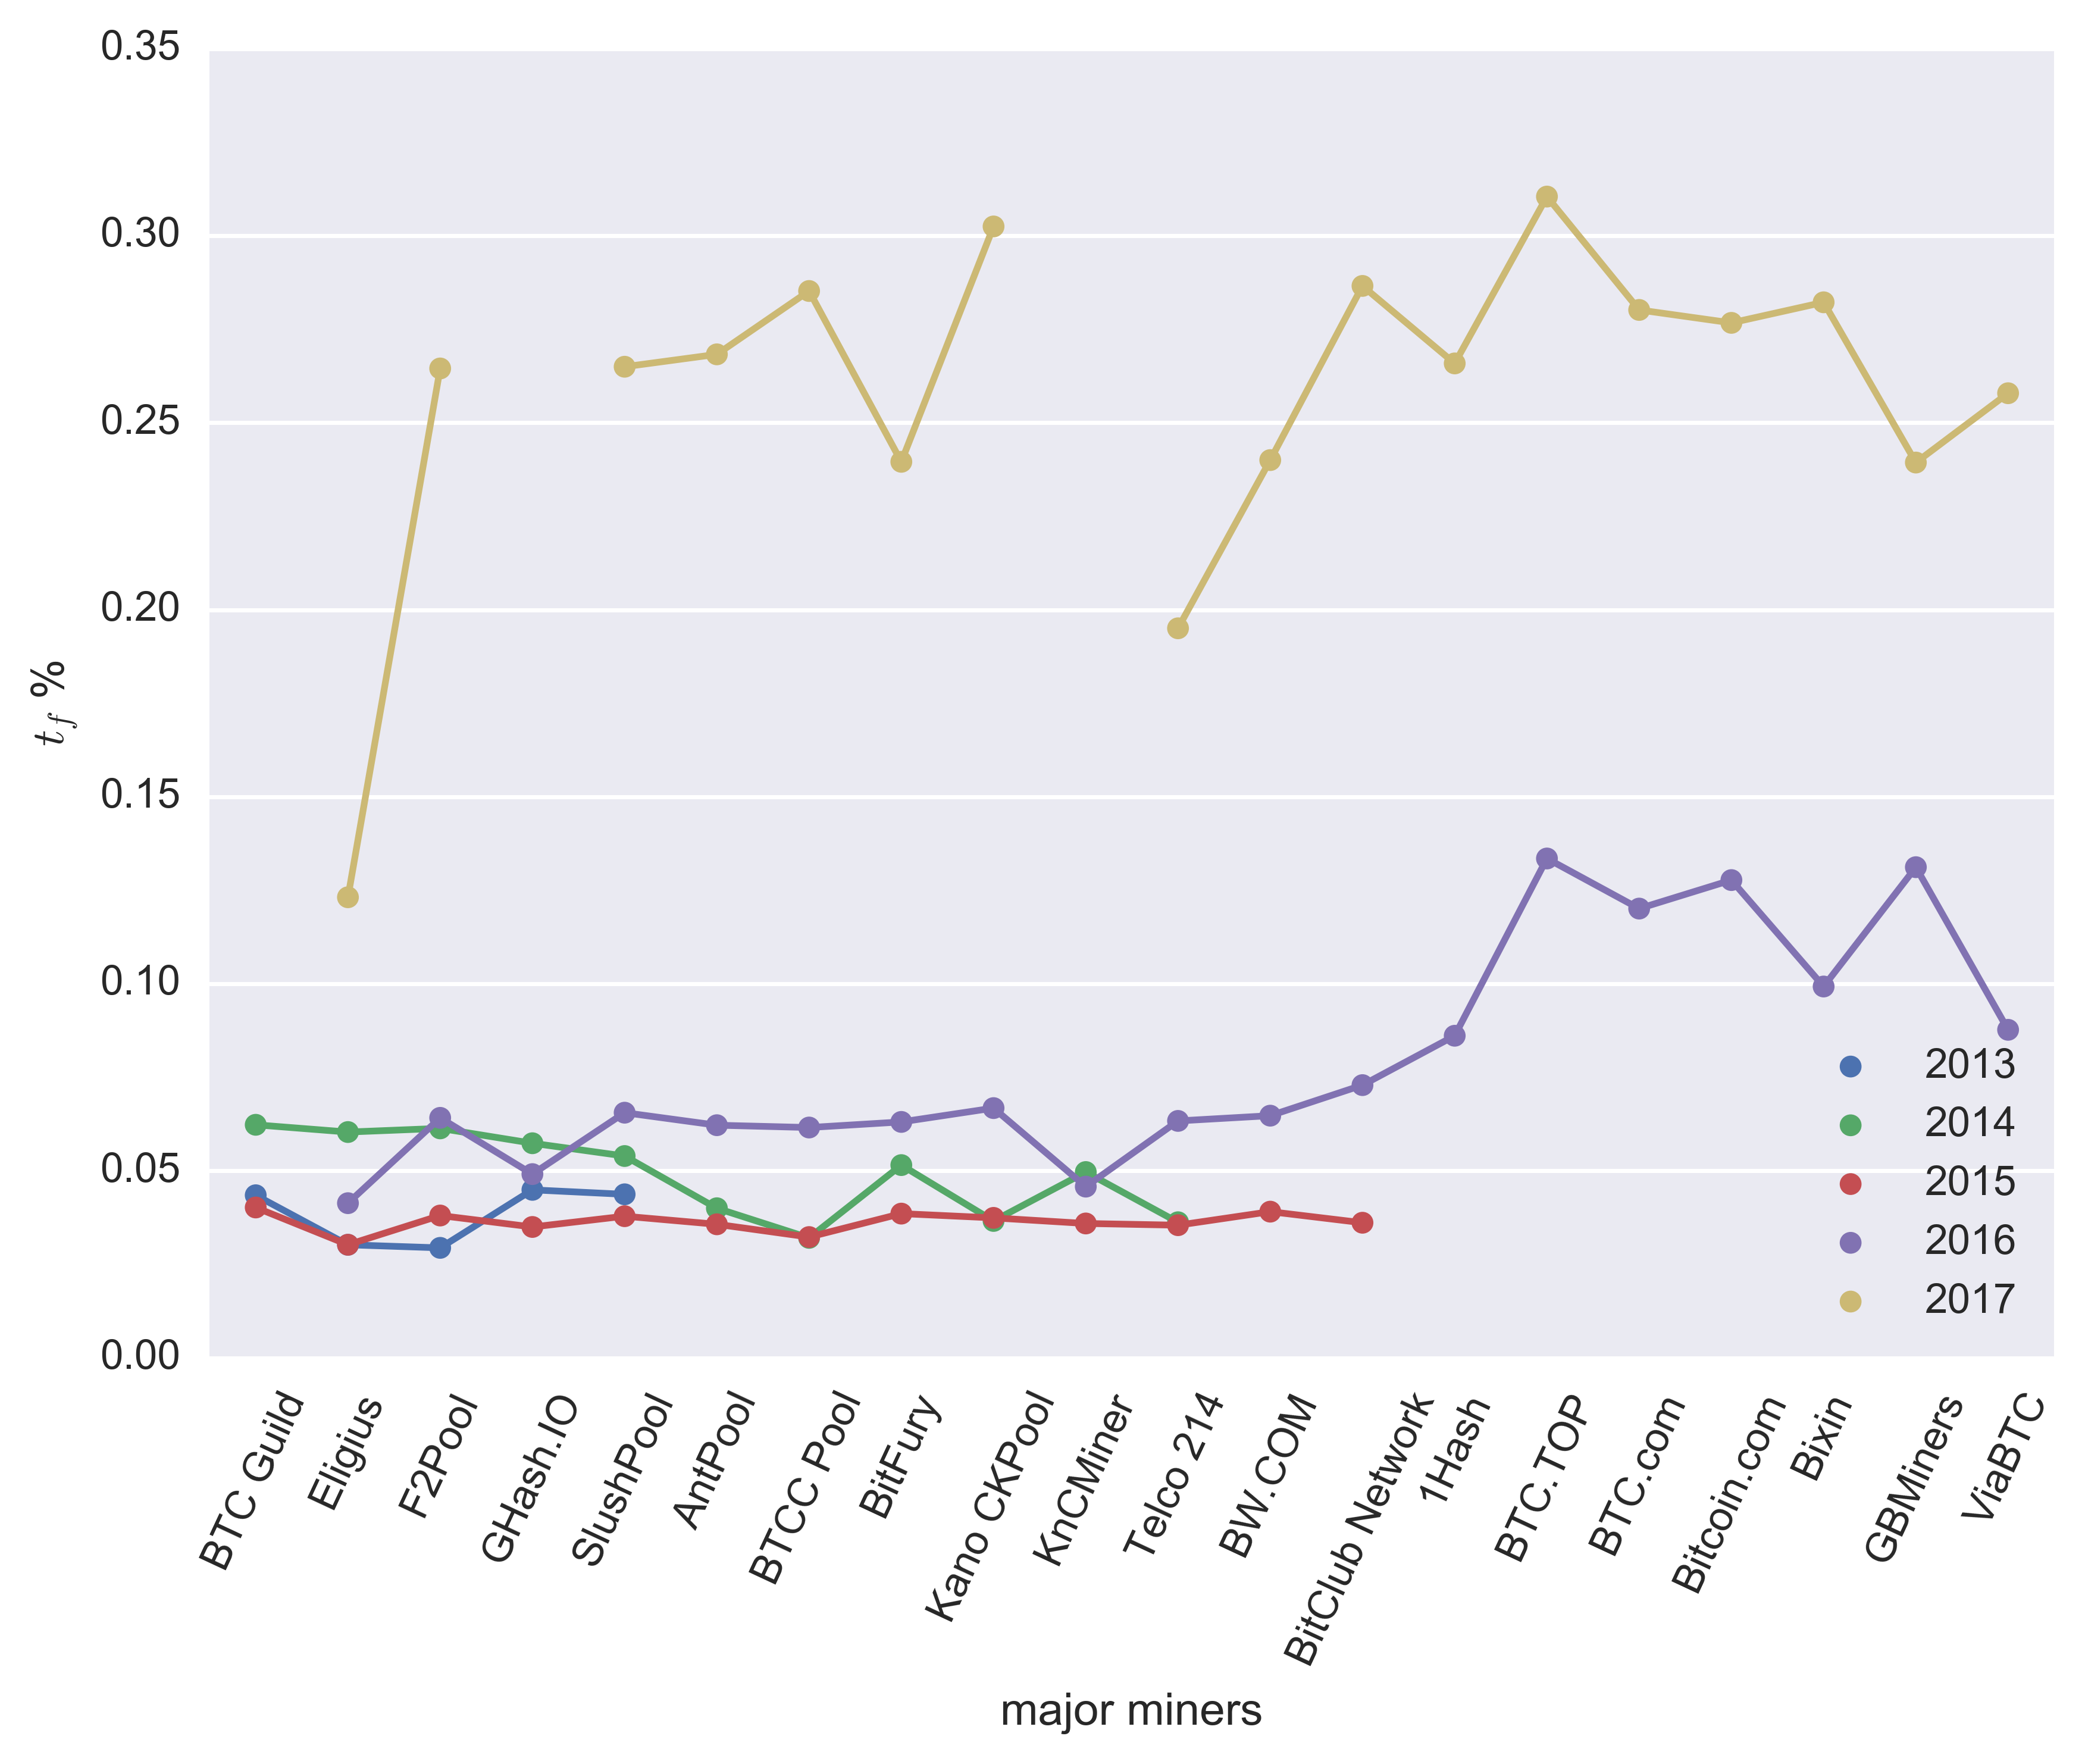
\includegraphics[width=1\textwidth]{img/fee_input_miners}
	\caption{Average \% of $t_f$ paid from users to the top $20$ miners of all times, grouped by year.}
	\label{fig:fee_input_miners}
\end{figure}

%TODO: TALK ABOUT 0-FEE TRANSACTIONS
\section{Is Bitcoin a Green-Wise Choice?}
After calculating the miner's consumption related
to the revenue we are concerned to know
which is the impact of Bitcoin network on the environment.
To know the electricity cost of mining in the Bitcoin
network is necessary to know exactly how many
miners are running and how much is their
consumption. Unfortunately
no one really knows how many
miners are active and running in the network
and this number changes every day, plus we don't
have information about which miner's hardware is
used but we could estimate
they are in the order of hundred thousands, they group in
mining pools and we could consider they are using
the most powerful mining hardware on market
at the time of analysis which is AntMiner~S$9$.
The problem of consumption
is that, even if there are hundreds, thousands or ten
thousands of miners in the network, they will approve
anyway $3$-$4$ transactions per second but they will use, accordingly,
more consumption of electricity.
Now, if we make assumptions on transaction consumption,
considering a relatively low number of miners, with peaks
of one hundred fifty thousand and all of them using AntMinerS$9$,
we would have a consumption between $400$ and
$500$\,Kwh per transaction, and if we grant that an
average consumption of a house in the United States,
which is one of the highest in the world, is of
$11000$\,Kwh per year, consuming then about
$30$\,Kwh per day, we can say
that Bitcoin is anything
but a green choice.
The problem of Bitcoin consumption is that
it only depends on how many miners are
active in the network and if the Bitcoin price
is rising then there could be more eager
individuals willing to join, causing an increment
of the difficulty to solve the proof-of-work so
the system is anyways able to produce
blocks every $10$ minutes
with a defined maximum size of $1$\,\gls{mb},
but the overall consumption of the network
will be higher. So every time the difficulty
is raised also the consumption will increase
accordingly.
It might be good then to mine in places
where the electricity is produced using
renewable energy and also trying to avoid
the inclusion of stand alone
miners, otherwise they would work without
ever mine a block, consuming a lot of energy.
Even if our evaluation shows a downward estimation,
the Bitcoin economy has a consumption
only of a thousandth if compared to the
whole oil industry per hour.
We estimate for Bitcoin a consumption
of $4.32$\,Gwh per hour while in the Statistical
Review of World Energy from BP\,\cite{BPSRWE2016}
they show that the oil industry has a consumption
of $5600$\,Gwh per hour. Until Bitcoin
would be that competitive for eager miners, then
the difficulty is intended to grow leading
the cryptocurrency into a really costly and
consuming scenario, plus always less miners
will be able to enjoy reward benefits and they will
end up mining for nothing with more
electricity consumption and consequence of that
would be the increment of the fees, but that would
attract even more miners and here we are at the earlier
scenario. A solution to that might be to regulate
the miners traffic
by controlling and auto-adjusting
the number of miners which
can join the network, in
that way the fees are contained and
regulated, having also a content consumption.

\chapter{Conclusion}
\label{chap:conclusion}
This Chapter aims to highlight the most relevant
observations while running \gls{bas}
and to proof whether our assumptions were
accurate or not, providing an explanation and also an
estimation of how the system might change in the next years.
We compare previous results with ours and we give
opinions on the hot topics in Bitcoin, regarding
the block size, the fees and miner's profit and then we
discuss and test the accuracy of our prediction models.
We evaluate that scalability issues brought to a 
centralization problem. When it comes
about mining, the scenario changes from distributed
to decentralized because of mining pools.
Then we state that in order to increase
the system performance and
scalability an eventual change on $\mathcal{T}$
and $Q$ should be considered with all the
advantages and disadvantages that these changes
might lead to.
Finally we generate prediction models about the
miner's profit and the transaction latency according
to the fee paid and the fee density for each
transaction, and this is profitable either for
miners and users so the firsts need
to have a guaranteed gain in mining while
the seconds need to get a faster
confirmation time by optimizing
their fees.
\section{Results}
\label{sec:results}
%Scalability
When Bitcoin was first implemented, one of its strength was
the decentralization. Miners could join the network all
over the world and more miners meant a more secure
network. During the years though, the reward enticed
always more people around the world and new miners
kept joining the network increasing in that way the
difficulty to solve the puzzle, since the creation time
should be kept fixed at $10$\,minutes. Consequently,
the Bitcoin hashing power kept growing, so
it became more difficult for single individuals to
mine new blocks, decreasing in that way the
chances for miners to gain their reward and leaving
space in the network to mining pools, since
they can gather up miners as well
as their hashing power.
This led to a scenario where singular
individuals need to join bigger mining
pools and the whole network changed
from distributed to decentralized since
mining pools are controlled by third parties
society so they control a big portion
of the hashing power needed to mine new blocks.
Furthermore, large mining pools nowadays
withhold information about number of miners,
the hardware they use or they profit,
making the centralization in the system
even more enhanced. Being one of Bitcoin
value proposition trustlessness, Bitcoin is only useful
if is decentralized, since centralization requires trust.
The other problem in scalability regards the amount
of transactions to be approved every day by the
Bitcoin system, and we have seen that
this number is constrained by
$Q$, $\mathcal{T}$ and $t_q$ and
since the transaction size will always be
around $400$-$500$\,bytes, we consider
a change in the block size $Q$ and
in the block creation time $\mathcal{T}$.
Table~\ref{tab:scalability_results} shows
the results and our assumptions after a
longitudinal study on the Bitcoin
blockchain. Decreasing $Q$ might
appear a good solution for the number
of advantages it has,
but the only two disadvantages are critical
for both performance and
scalability matters, while it could be
much easier to deal
with the orphan rate amplification.
For that reason
a decrease on the block size is ill-judged.
We have instead an opposite scenario
with the block creation time. An increment
would be ill-judged since the system will
not be scalable, will be less performing and
miners will have less profit while mining
with the only advantage to have a lower
orphaning rate.

\begin{table}
	\centering
	\caption{Scalability and performance scenario and consequences if block size $Q$ and block creation time $\mathcal{T}$ are increased or decreased.}
	\label{tab:scalability_results}
	\begin{tabular}{|m{0.4cm}|m{4.8cm}|m{4.8cm}|}
	\cline{2-3}
	\multicolumn{1}{c|}{}&
	\multicolumn{1}{c|}{\textbf{Higher $\uparrow$}} &
	\multicolumn{1}{c|}{\textbf{Lower $\downarrow$}} \\ \hline
		 \textbf{$Q$}&\begin{itemize}
			\item [$+$] more scalability and transactions accepted per day
			\item [$+$] less latency $t_l$
			\item [$-$/$+$] lower fees, good for users bad for miners
			\item [$-$] orphan rate amplification
			\item [$-$] damage to centralization
			\item [$-$] congestion concern solved
			with transaction eviction by miners
			\item [$-$] temporary solution
		\end{itemize}&\begin{itemize}
			\item [$+$] no transaction spam
			\item [$+$] no $0$-fee transactions
			\item [$+$] less mining cost
			\item [$+$] less propagation time
			\item [$+$] less chance of orphaning
			\item [$-$/$+$] higher fees, good for miners bad for users
			\item [$-$] less throughput
			\item [$-$] more latency $t_l$
		\end{itemize}\\ \midrule
		\hline
		\textbf{$\mathcal{T}$}&\begin{itemize}
			\item [$+$] orphaning rate much lower
			\item [$+$] no physical changed needed to support faster inner node communication
			\item [$-$] lower throughput $\gamma$ unless $Q$ is increased
			\item [$-$] system not very scalable unless $Q$ is increased
			\item [$-$] profit $\langle \Pi \rangle$ is confined
		\end{itemize}& \begin{itemize} %TODO: T does not affect the users that much (maybe in t_l)
		\item [$+$] higher throughput $\gamma$
		\item [$+$] system is more scalable
		\item [$+$] profit $\langle \Pi \rangle$ much higher for miners
		\item [$+$/$-$] not much information about $t_l$ but for sure it will not drastically increase
		\item [$-$] faster inner node communication is required with possible changes in the physical structure
		\item [$-$] exponential increment of orphaning rate
	\end{itemize}\\
		\hline
	\end{tabular}
\end{table}

%\subsection{Performance}
As we can observe from Table~\ref{tab:scalability_results},
throughput $\gamma$ increase when either
the block size $Q$ is raised or the creation time
$\mathcal{T}$ is lowered, a good compromise of both
might be the solution to part of the scalability and
performance problems in the Bitcoin network.
According to Croman et al.\,\cite{croman2016},
the block size should not exceed $4$\,\gls{mb}
given a creation time of $10$\,minutes. We assume
that a good compromise could be to increase the
block size limit at $1.5$\,\gls{mb} and lower the
creation time at $8$\,minutes. In that way
the system will perform an average of $5$-$6$
transactions per second with a creation time of $10$\,minutes,
reaching $10$ transactions per second if the $8$\,minutes
interval is respected.

While we can not define a relation between
$Q$ and $t_f$, since they are related only
when a drastic change in the block size is made
in the network, we can state that, from
$2013$ to $2017$ the relation between $t_f$
and $t_l$ day by day more noticeable, having
almost an inverse proportionality in the latest data
from $2017$ as displayed in
Figure~\ref{fig:fee_latency}.
We represent this relation with
Equation~\ref{eq:latency_function}.
In $2017$ $0$-fee transactions almost disappeared from
the system and that is due to the incredibly high
latency they were facing, since it took
an average of $33$\,hours to
get confirmed and included in a block
by some miner. If only this fee is raised
less than $0.0002$\,\bitcoinA,
the transaction latency drops to an average
of $5$\,hours, and with a fee between
$0.0008$\,\bitcoinA~and $0.001$\,\bitcoinA~the
average expected latency is less than
$1$\,hour.

%\subsection{Fees and Tolls}
Regarding fees and tolls in the network
we estimate the profit of a miner
using AntMiner~S$9$\,\cite{antminerS9}
as mining hardware.
We put in a relation the profit of a single
block mined with its creation time.
Once we collected enough data and calculated
the profit, we inferred a possible trend for
$\langle \Pi \rangle$ and called it \emph{Miner Profit Function},
$f_{\langle \Pi \rangle}$. We used Numpy libraries\,\cite{scipy}
for the interpolation (Appendix~\ref{lst:interpolation})
and we perform a regression of
$2$ and $39$ degrees function
to see how the trend
changes if the polynomial level is increased.
Figure~\ref{fig:profit_creation_time} shows
both functions interpolated plus the samples
for each block in $2017$ and we define
$f^2_{\langle \Pi \rangle}$
in Equation~\ref{eq:miner_profit} while
we use $f^{39}_{\langle \Pi \rangle}$ more
like a reference to set our boundaries
and see where the profit
tend to increase or maintain its value
after a certain amount
of time. We state
that for the first $2$\,minutes
and after $20$\,minutes
is not profitable to produce new
blocks, while is good to have a creation
time between $3$ and $8$\,minutes.
We finally tested the accuracy of our
Miner Profit Function, $f^2_{\langle \Pi \rangle}$,
using scikit-learn libraries\,\cite{scikit-learn}
and calculating the \gls{mae} as shown in
Appendix~\ref{lst:mae}. We considered
then as predictors, our dataframe $D$,
and we used as target values for
accuracy tests, data retrieved on a newer portion
of the blockchain for every blocks occurred
between the $4^{\text{th}}$ and
the~$11^{\text{th}}$ of November $2017$,
and they turned out to have
a median absolute error of
\gls{mae}~$= 0.00002455$\,\bitcoinA.

The other two functions inferred
are shown in Equations~\ref{eq:latency_function},
\ref{eq:feedensity_latency_function} and they
try to optimize users' bandwidth according
to the fee these users are willing to pay
for their transactions.
Like in the Miner Profit Function,
we evaluate a polynomial level of $2$ and $39$
degrees, and while the first one is the reference for our
prediction models $f^2_{t_f}$ and $f^2_{\rho}$,
the second one is useful to give us an idea about the boundaries
of these models. Unfortunately, since rules behind
the inclusion in a block are not yet well defined, and mining
pools could change these rules, for example
they possibly have changed the transaction eviction
for $0$-fee transactions to an eviction
for the $0$-$\rho$ transactions, and the block
is generated after a random number of minutes,
the predictions on the available bandwidth
for users are not as accurate as the one for
the miners' profit, having an \gls{mae}~$= 1.2$\,hours
in $f^2_{t_f}$ and an \gls{mae}~$= 1.03$\,hours
in $f^2_{\rho}$. We ran these tests, as in the
Miner Profit Function, in a
newer portion of the blockchain,
between the $4^{\text{th}}$ and
the~$11^{\text{th}}$ of November $2017$.
However, thanks to our $f^{39}$ interpolation
we can define the boundaries in which this functions
are reliable, plus, Figure~\ref{fig:fee_latency}
gives a good overview of the transaction
approval time trend in relation to the fee paid
and according to both measurements,
paying more than $0.001$\,\bitcoinA~would
be non profitable for users.
Furthermore, we believe that nowadays miners
changed their inclusion rules from a priority
on $t_f$ to a preference on $\rho$, this is the
reason for us to infer also $f^2_{\rho}$.
However, fee density is not dependent
form users, since it is calculated considering
also the transaction size $t_q$. For that reason, users
should tend to consider a $t_f = 0.001$\,\bitcoinA~as the limit
for their fees, no matter how much is the amount
transferred.

%TODO: CONTINUE

\section{Discussion}
\label{sec:discussion}
Despite the withhold of information form mining pools
and the difficulty in retrieving the blockchain, containing
sometimes not convincing data, e.g. a negative creation time
for some blocks mostly before $2013$, we are satisfied about
our studies and the results obtained. We managed to
perform a longitudinal study on the Bitcoin blockchain,
analyzing more transactions than any previous work,
collecting recent data of $2017$ and combining
different data sources to get even more information, all
stored in our data structure that aims to give
all the information regarding blocks and transactions, saving
up $10$\,times the amount of disk space.
We could also, using machine
learning techniques, infer useful functions effective for
both users and miners, in order to gain more profit
out of the mining process.
Creating our
data analytics system
might not have been the easiest solution,
but it was the one which allowed us to retrieve
the exact information we wanted without storing the whole
blockchain. We had trouble using Bitcoin's \gls{api}
since the website was not always available plus
it prevents from having too many requests at
the same time; because of that we spent more than a month
to be able to retrieve all the information
we wanted and to find a way to store them
nicely in a way to be easily retrieved.
With all the data collected and our data structure
$D$ we were able to verify our assumption
on scalability, performance and finally
to generate prediction models that even if
are constrained and reliable only for a small interval
of data input, they give an idea of how entities
should behave in Bitcoin system.

Despite we inferred our models, giving
information on how miners and users could use their time
and money, the creation time $\mathcal{T}$
is still a random process, determined by the proof of work,
and how lucky miners are to find the solution. Because of that,
paying so much fee, $t_f$, will not guarantee
an extremely fast execution, but at least your
transaction will be considered as "high priority"
in more mining pools according to the amount of its $t_f$.

It is also important to note that the problem of scalability
has been taken into serious consideration and nowadays
smart contracts like \gls{rsk}\,\cite{rsk} are
emerging, claiming to scale almost as much as PayPal even
though they are not still in common use and
maybe more testing on those will be necessary.

And finally, the problem of consumption is also
urgent, moving also prominent characters such as
Bram Cohen (inventor of BitTorrent) to launch
new green cryptocurrencies such as \emph{Chia}\,\cite{chia},
since he claims that
a Bitcoin transaction wastes as much as electricity
as it takes to power an American home
for a week, and we tested that it might be true,
comparing the Bitcoin system to the whole
oil industry.

Another issue while performing the longitudinal
study was the pricing and money value of Bitcoin.
It's hard to make prediction when the
currency is affected by such
high volatility. Usually the Bitcoin
price tends to raise if there is an unstable
situation in the global market and it frequently
goes down when Bitcoin currency is involved
in scandals such as the bankrupt of Mt Gox\,\cite{mtgox_news},
once the biggest Bitcoin exchange on the market,
money laundering and black marked related
issue, since people are willing to spend
less money in Bitcoin if something like that happens
in the system.

\section{Future Implementation}
\label{sec:future_implementation}
By profiling \gls{bas} we were able to understand what
we could improve. For performance evaluation
we used a line-by-line profiling for
Python\,\cite{line_profiler}, displayed
in Appendix~\ref{app:profiling}.
We divided the computation in plot and
retrieval, then retrieval in fetch and write.
The fetching of data takes the $85.5$\%
of the total time, while
the writing of data only the $13.8$\%.
The $99.9$\% of the computation in
data fetching is due to the \gls{api} calls
on \url{blockchain.info}. For that reason, the system
still suffers in performance but
we could get faster latency in the future
if we alter the primitives of data retrieval
in a way to have bigger portions retrieved
and less connections to establish.

Further analyses should take into consideration a more accurate
estimation about the impact Bitcoin has on the environment.
This could be done by studying
the number of miners in the network and which kind of
mining software is used, even if these data are kept
secret by mining pools.
The fact is, that Bitcoin has an high
electricity consumption and it is intended to grow along
with the Bitcoin hashing rate, so further studies and
concerns about this topic should be considered and we believe that
in the near future, the focus on cryptocurrencies
will address in that direction.

A future useful feature of \gls{bas} might be a \emph{short-time model
prediction}. We thought about it as a
retrieval of the last weekly transactions in the system,
then, a real time model is generated, giving to users information about
the fee they should pay in order to
optimize their latency at a reasonable costs.

\bibliographystyle{plain}
\bibliography{thesis}

\begin{appendices}

\chapter{Other Definitions}
\label{app:otherdefinitions}
\begin{description}
	\item[full node:] in a decentralized
	digital currency peer-2-peer network, is a node that stores
	and processes the entirety of every block,
	storing locally the entire size of the blockchain.
	\item[light node:] in a decentralized
	digital currency peer-2-peer network, is a node that only
	stores the part of the blockchain it needs.
	\item[satoshi:] Unit of the Bitcoin currency.
	100,000,000 satoshi are 1 \bitcoinA.
	\item[$51$\% Attack:] 51\% refers to an attack on a blockchain,
	by a group of miners
	controlling more than 50\% of the network's mining hash rate, or
	computing power. The attackers would be able to prevent new
	transactions from gaining confirmations, allowing them to halt
	payments between some or all users. They would also be able
	to reverse transactions that were completed while they were in
	control of the network, meaning they could double-spend coins.
	They would almost certainly not be able to create
	new coins or alter old blocks, so a 51\% attack
	would probably not destroy Bitcoin or another
	blockchain-based currency outright,
	even if it proved highly damaging\,\cite{51attack}.
	
\end{description}


\chapter{List of Symbols}
\label{app:LOS}
\begin{description}[leftmargin=!, labelwidth=\widthof{\bfseries $M_{demand}(b)$ }]
	\setlength\itemsep{1em}
	\item [$t_B$] number of transaction approved in a block $B$.
	\item [$t_{in}$] transaction input in bitcoin (\bitcoinA). All the money sent.
	\item [$t_{ou}$] transaction output (\bitcoinA). All the money received.
	\item [$t_{f}$] transaction fee (\bitcoinA) (Equation~\ref{eq:txfee}).
	\item [$t_q$] transaction size, in bytes.
	\item [$t_l$] commit latency of a single transaction (seconds, minutes, hours) (Equation~\ref{eq:txlatency}).
	\item [$t_h$] transaction height. Height of the block in which the transaction is included.
	\item [$t_{ha}$] transaction hash.
	\item [$t_\%$] percentage of $t_{in}$ paid in fee, $t_f$.
	\item [$\mathcal{T}$] expected block interval time~($\sim$\,$10$\,min)
	\item [$\mathbb{P}_{orphan}$] probability that given a block is orphaned.
	\item [$\tau$] block solution propagation time, we consider a $\tau = 15.7$\,
	seconds according to Croman\,\cite{croman2016}. %TODO: analyze recent data form Croman
	\item [$t_{epoch}$] timestamp of a transaction $t$.
	Epoch of when $t$ was first seen in the network
	\item [$\eta$] cost per hash.
	\item [$\langle \Pi \rangle$] expectation value of a miner’s profit per block.
	\item [$\langle V\rangle$] expectation value of a miner’s revenue per block.
	\item [$\langle C\rangle$] expectation value of a miner's hashing cost per block.
	\item [$R$] block reward, currently at 12.5 \bitcoinA, halved every $210,000$ blocks.
	\item [$h$] miner's individual hash rate.
	\item [$H$] total hash rate of Bitcoin network.
	\item [$Q$] block size or block space in bytes/\gls{mb}.
	\item [$Q^*$] the block size that maximizes the miner’s expected profit.
	\item [$\rho$] fee density, or the price per byte for block space. (sat/byte).
	\item [$M$] money in \bitcoinA. Sum of all $t_f$ in a block.
	\item [$M_{demand}(b)$] partial sum of the $b$ transaction fees
	in mempool in order of descending fee density.
	\item [$M_{supply}(Q)$] miner’s cost due to orphaning to produce a certain block size $Q$.
	\item [$\mathcal{N}$] the set of transactions in a miner’s mempool.
	\item [$n$] number of transactions in a miner’s mempool.
	\item [$B$] single block.
	\item [$B_t$] transaction root that links to every transaction in a block $B$.
	\item [$B_{epoch}$] timestamp of a block $B$.
	Epoch of when the block was included in the blockchain
	\item [$B_h$] block height.
	\item [$B_{ha}$] block hash.
	\item [$B_{mi}$] miner which mined the block $B$.
	\item [$\gamma$] throughput of Bitcoin network, measured in transactions per second.
	\item [$D$] data frame generated by \gls{bas}.
\end{description}

\chapter{BAS Source Code}
\label{app:listing}
The complete source code can be found at: \url{https://github.com/ted92/Bitcoin-Analytics-System}.
\lstset{language=Python,
	basicstyle=\ttfamily,
	keywordstyle=\color{blue}\ttfamily,
	stringstyle=\color{red}\ttfamily,
	commentstyle=\color{green}\ttfamily,
	breaklines=true,
	morecomment=[l][\color{magenta}]{\#},
	label = {lst:dataframe}
}
\begin{lstlisting}[numbers=left,frame=single,caption={Creation of Pandas data frame}]
import pandas as pd
# a1, a2, a3 = lists of attributes
df = pd.DataFrame.from_items([('label1', a1), ('label2', a2), ('label3', a3)])
\end{lstlisting}

\lstset{language=Python,
	basicstyle=\ttfamily,
	keywordstyle=\color{blue}\ttfamily,
	stringstyle=\color{red}\ttfamily,
	commentstyle=\color{green}\ttfamily,
	breaklines=true,
	morecomment=[l][\color{magenta}]{\#},
	label = {lst:dataframeunion}
}
\begin{lstlisting}[numbers=left,frame=single,caption={Union of df1 and df2 in a new data frame new\_df }]
# df1, df2 = DataFrame
new_df = pd.concat([df1, df2])
\end{lstlisting}


\lstset{language=Python,
	basicstyle=\ttfamily,
	keywordstyle=\color{blue}\ttfamily,
	stringstyle=\color{red}\ttfamily,
	commentstyle=\color{green}\ttfamily,
	breaklines=true,
	morecomment=[l][\color{magenta}]{\#},
	label = {lst:dataframegroupby}
}
\begin{lstlisting}[numbers=left,frame=single,caption={Group by attributes 'a1' and 'a2'. After that the mean, the sum and the median is calculated on the other attributes. The method reset\_index() returns a data frame with the original attributes before the groupby was applied. }]
grouped_df = df .groupby(['a1', 'a2']).mean().reset_index()
grouped_df2 = df.groupby(['a1', 'a2']).sum().reset_index()
grouped_df2 = df.groupby(['a1', 'a2']).median().reset_index()
\end{lstlisting}


\lstset{language=Python,
	basicstyle=\ttfamily,
	keywordstyle=\color{blue}\ttfamily,
	stringstyle=\color{red}\ttfamily,
	commentstyle=\color{green}\ttfamily,
	breaklines=true,
	morecomment=[l][\color{magenta}]{\#},
	label = {lst:dataframesize}
}
\begin{lstlisting}[numbers=left,frame=single,caption={Count how many occurrences for the attribute 'a1' and save this number in a new attribute called 'size'.}]
df = df.groupby('a1').size().to_frame('size').reset_index()
\end{lstlisting}


\lstset{language=Python,
	basicstyle=\ttfamily,
	keywordstyle=\color{blue}\ttfamily,
	stringstyle=\color{red}\ttfamily,
	commentstyle=\color{green}\ttfamily,
	breaklines=true,
	morecomment=[l][\color{magenta}]{\#},
	label = {lst:epochdatetime}
}
\begin{lstlisting}[numbers=left,frame=single,caption={Function for data manipulation. It creates a new column ('date'), from another ('B\_ep') containing the respective $B_{epoch}$ transformed in date time value with days as granularity.}]
def epoch_date_dd(df):
  # get a data frame with a column of epoch 'B_ep', returns
  # another column with the date yyyy-mm-dd so it
  # orders the date by day
  # :param df:  dataframe in input
  # :return:    new dataframe containing the 'date' attribute
  df['date'] = df['B_ep'].apply(epoch_datetime)
  df['date'] = df['date'].apply(revert_date_time)
  df['date'] = df['date'].str.slice(start=0, stop=10)
  return df
\end{lstlisting}


\lstset{language=Python,
	basicstyle=\ttfamily,
	keywordstyle=\color{blue}\ttfamily,
	stringstyle=\color{red}\ttfamily,
	commentstyle=\color{green}\ttfamily,
	breaklines=true,
	morecomment=[l][\color{magenta}]{\#},
	label = {lst:jsonretrieval}
}
\begin{lstlisting}[numbers=left,frame=single,caption={Data retrieval using \gls{rest}ful \gls{api}s provided from \url{blockchain.info}.}]
import urllib2
import json
global block_hash_url
block_hash_url = "https://blockchain.info/rawblock/"

def get_json_request(url):
  # Read the url and get json data.
  # :param url: str, site where to fetch information
  # :return: str, data requested in json format
  json_req = urllib2.urlopen(url).read()
  request = json.loads(json_req)
  return request

# get a block given a hash
block = get_json_request(block_hash_url + hash)

# get the previous block through block attribute 'prev_block'
hash = block['prev_block']
\end{lstlisting}

	\lstset{language=Python,
	basicstyle=\ttfamily,
	keywordstyle=\color{blue}\ttfamily,
	stringstyle=\color{red}\ttfamily,
	commentstyle=\color{green}\ttfamily,
	breaklines=true,
	morecomment=[l][\color{magenta}]{\#},
	label = {lst:block}
}

\begin{lstlisting}[float, numbers=left,frame=single,caption={Block object structure obtained using Bitcoin's \gls{api}s},language=Python]
class Block:
  def __init__(self, b):
    self.hash = b['hash']
    self.version = b['ver']
    self.previous_block = b['prev_block']
    self.merkle_root = b['mrkl_root']
    self.time = b['time']
    self.bits = b['bits']
    self.fee = b['fee']
    self.nonce = b['nonce']
    self.n_tx = b['n_tx']
    self.size = b['size']
    self.block_index = b['block_index']
    self.main_chain = b['main_chain']
    self.height = b['height']
    self.received_time = b.get('received_time', b['time'])
    self.relayed_by = b.get('relayed_by')
    self.transactions = [Transaction(t) for t in b['tx']]
    for tx in self.transactions:
        tx.block_height = self.height
\end{lstlisting}


	\lstset{language=Python,
	basicstyle=\ttfamily,
	keywordstyle=\color{blue}\ttfamily,
	stringstyle=\color{red}\ttfamily,
	commentstyle=\color{green}\ttfamily,
	breaklines=true,
	morecomment=[l][\color{magenta}]{\#},
	label = {lst:transaction}
}

\begin{lstlisting}[float, numbers=left,frame=single,caption={Transaction object structure obtained using Bitcoin's \gls{api}s.},language=Python]
class Transaction:
  def __init__(self, t):
    self.double_spend = t.get('double_spend', False)
    self.block_height = t.get('block_height')
    self.time = t['time']
    self.relayed_by = t['relayed_by']
    self.hash = t['hash']
    self.tx_index = t['tx_index']
    self.version = t['ver']
    self.size = t['size']
    self.inputs = [Input(i) for i in t['inputs']]
    self.outputs = [Output(o) for o in t['out']]

    if self.block_height is None:
       self.block_height = -1
\end{lstlisting}



	\lstset{language=Python,
	basicstyle=\ttfamily,
	keywordstyle=\color{blue}\ttfamily,
	stringstyle=\color{red}\ttfamily,
	commentstyle=\color{magenta}\ttfamily,
	breaklines=true,
	morecomment=[l][\color{magenta}]{\#},
	label = {lst:portionsretrieval}
}

\begin{lstlisting}[float, numbers=left,frame=single,caption={Portion retrieval having a jump $J = 10$ and a number of blocks retrieved per time $b = 10$.},language=Python]
global latest_block_url
latest_block_url = "https://blockchain.info/latestblock"

jump = 10
b = 10
if(os.path.isfile(name)):
  # retrieve data frame from name.csv file
  df = pd.DataFrame.from_csv(name, sep='\t')
  hash_list = df['B_h'].values
  # get the last height
  height_list = df['B_he'].values
  last_block = height_list[-1]
  # subtract the jump
  last_block = int(last_block) - jump
  # get the block where to start the new fetching
  b_array = get_json_request("https://blockchain.info/block-height/" + str(last_block) + "?format=json")
  blocks = b_array['blocks']
  b = blocks[0]
  #  lget the block hash that has to be fetched first
  block_hash = b['hash']
  # call the method for fetching the blockchain
  get_blockchain(b, block_hash)
else:
  # file does not exist
  # retrieve the last block hash
  latest_block = get_json_request(latest_block_url)
  block_hash = latest_block['hash']
  get_blockchain(b, block_hash)

\end{lstlisting}



	\lstset{language=Python,
	basicstyle=\ttfamily,
	keywordstyle=\color{blue}\ttfamily,
	stringstyle=\color{red}\ttfamily,
	commentstyle=\color{magenta}\ttfamily,
	breaklines=true,
	morecomment=[l][\color{magenta}]{\#},
	label = {lst:interpolation}
}

\begin{lstlisting}[float, numbers=left,frame=single,caption={Polynomial interpolation on miner's profit, $\langle \Pi \rangle$, and creation time, $\mathcal{T}$, using Numpy libraries.},language=Python]
x = df['B_T'].values
y = df['profit'].values
new_x, new_y, f = polynomial_interpolation(x, y, degree=2)

def polynomial_interpolation(x, y, degree=2):
  # given two lists of data it generates two new lists containing the y values interpolated
  # :param x : x values of the data to interpolate
  # :param y : y values of the data to interpolate
  # :param degree : polynomial degree
  # :return : x and y interpolated values. f is the polynomial.
  # order lists
  together = zip(x, y)
  sorted_together = sorted(together)
  x_vals = [el[0] for el in sorted_together]
  y_vals = [el[1] for el in sorted_together]
  # calculate polynomial
  z = np.polyfit(x_vals, y_vals, degree)
  f = np.poly1d(z)
  x_new = np.linspace(x_vals[0], x_vals[-1], len(x_vals))
  y_new = f(x_new)
  return x_new, y_new, f
\end{lstlisting}




	\lstset{language=Python,
	basicstyle=\ttfamily,
	keywordstyle=\color{blue}\ttfamily,
	stringstyle=\color{red}\ttfamily,
	commentstyle=\color{magenta}\ttfamily,
	breaklines=true,
	morecomment=[l][\color{magenta}]{\#},
	label = {lst:mae}
}

\begin{lstlisting}[float, numbers=left,frame=single,caption={\gls{mae} accuracy calculation on miner's profit $\langle \Pi \rangle$ calculated using scikit-learn libraries in Python.},language=Python]
from sklearn.metrics import mean_absolute_error
new_x, new_y, f = polynomial_interpolation(x, y, degree=2)
predicted = []
samples = df['B_T'].values
real = df['profit'].values
for float(s) in samples:
  predicted.append = f(s)
mae = mean_absolute_error(real, predicted)
\end{lstlisting}

\chapter{Profiling}
\label{app:profiling}
Performance of \gls{bas} using a line profiler for Python\,\cite{line_profiler}.
The profiling was evaluated running \gls{bas} on a small dataset $D$
with a size of $46$\,\gls{mb}.
We ran the profile on the \emph{main.py} class, to have an overall of the whole
\gls{bas} execution, then on the transaction retrieval
and writing, and finally, on the plotting of data.
Note that, for convenience, not all the lines are listed.
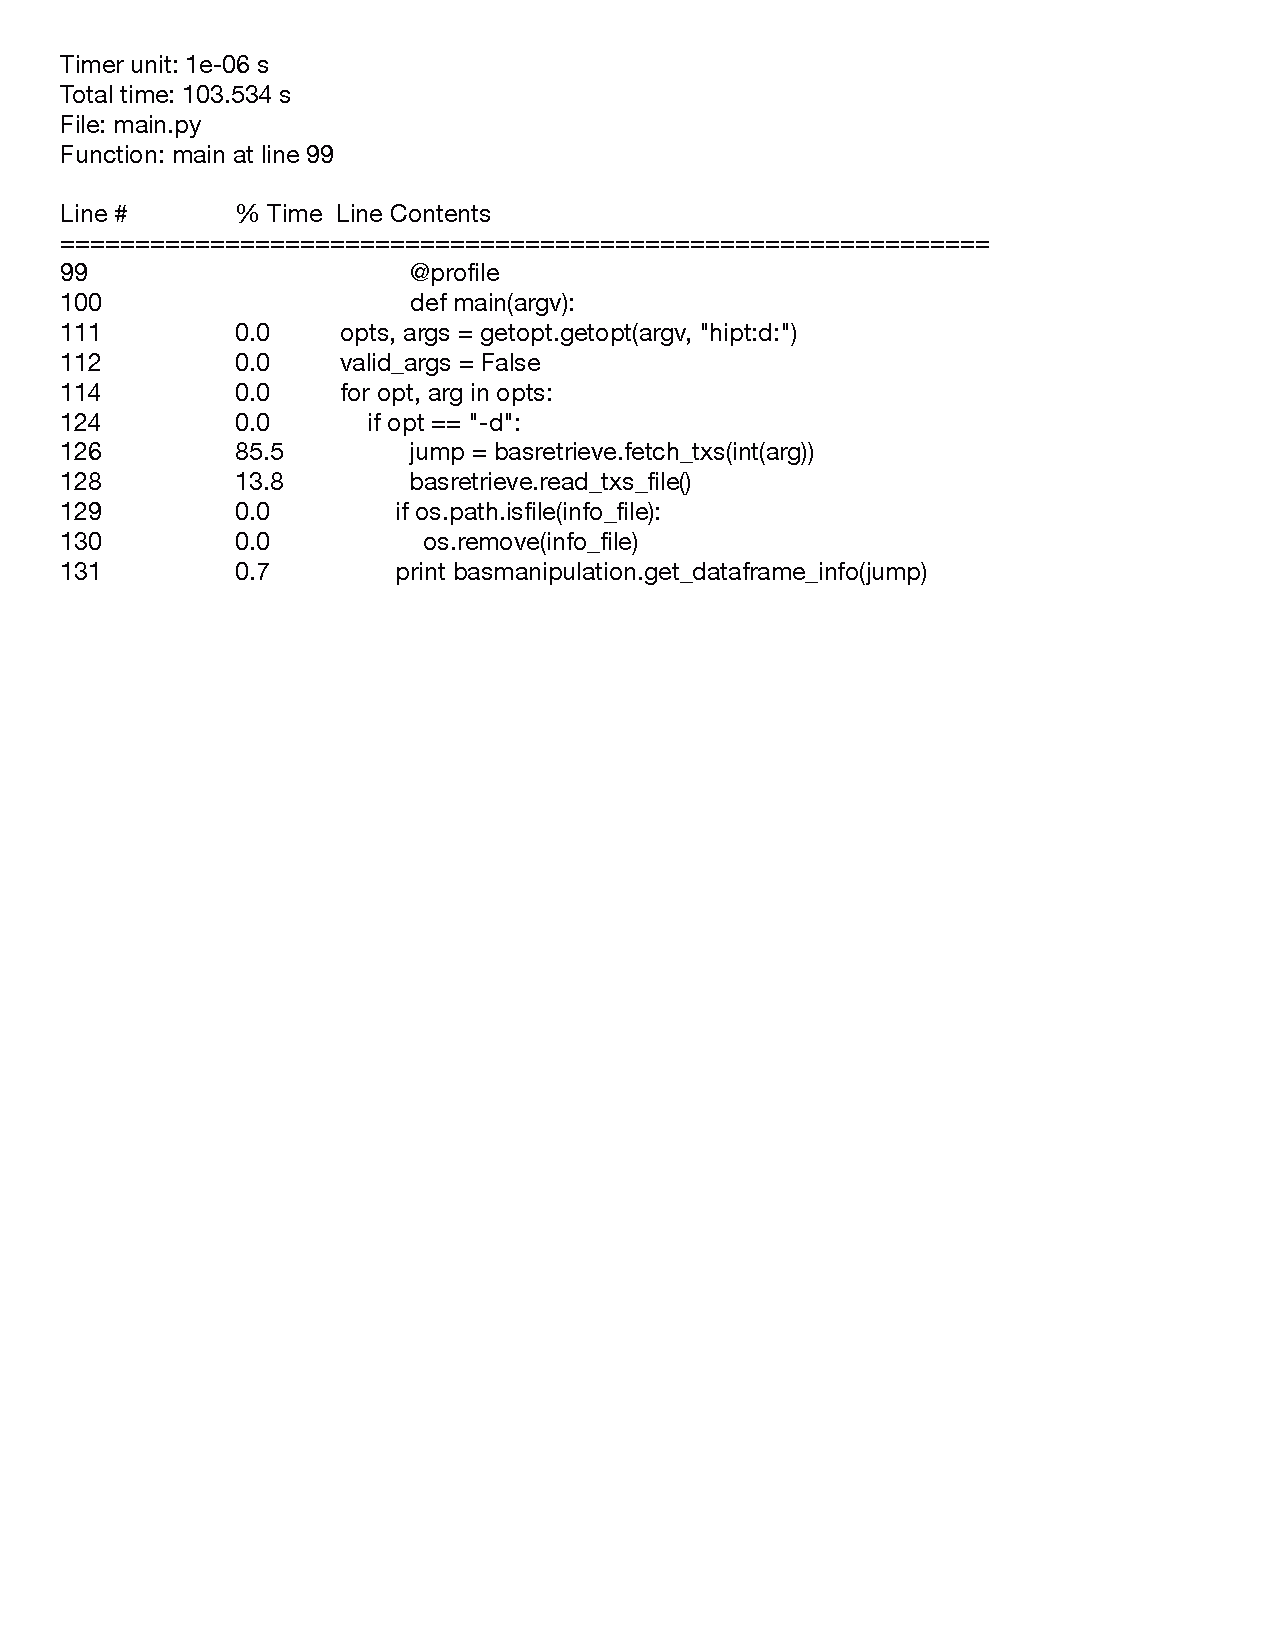
\includepdf[pages=-]{img/main_profile.pdf}
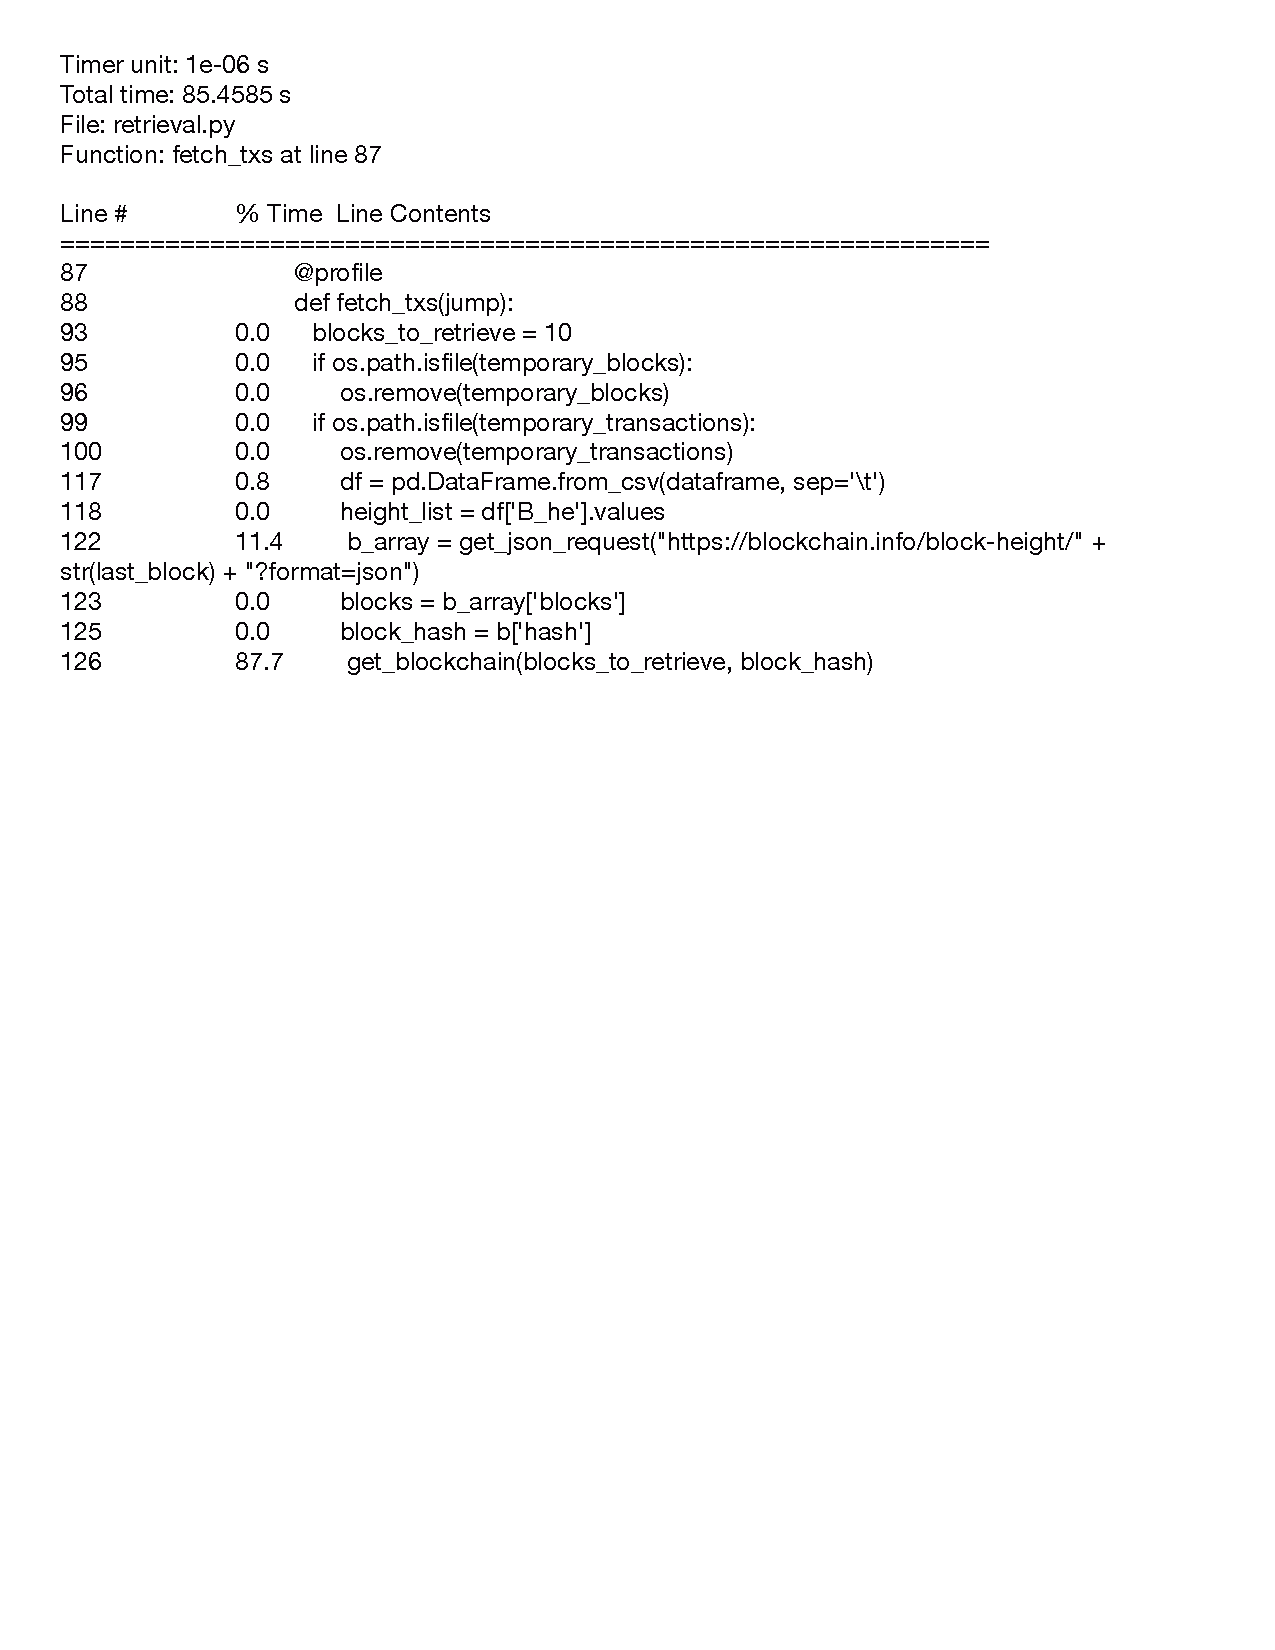
\includepdf[pages=-]{img/fetch_txs_profile.pdf}
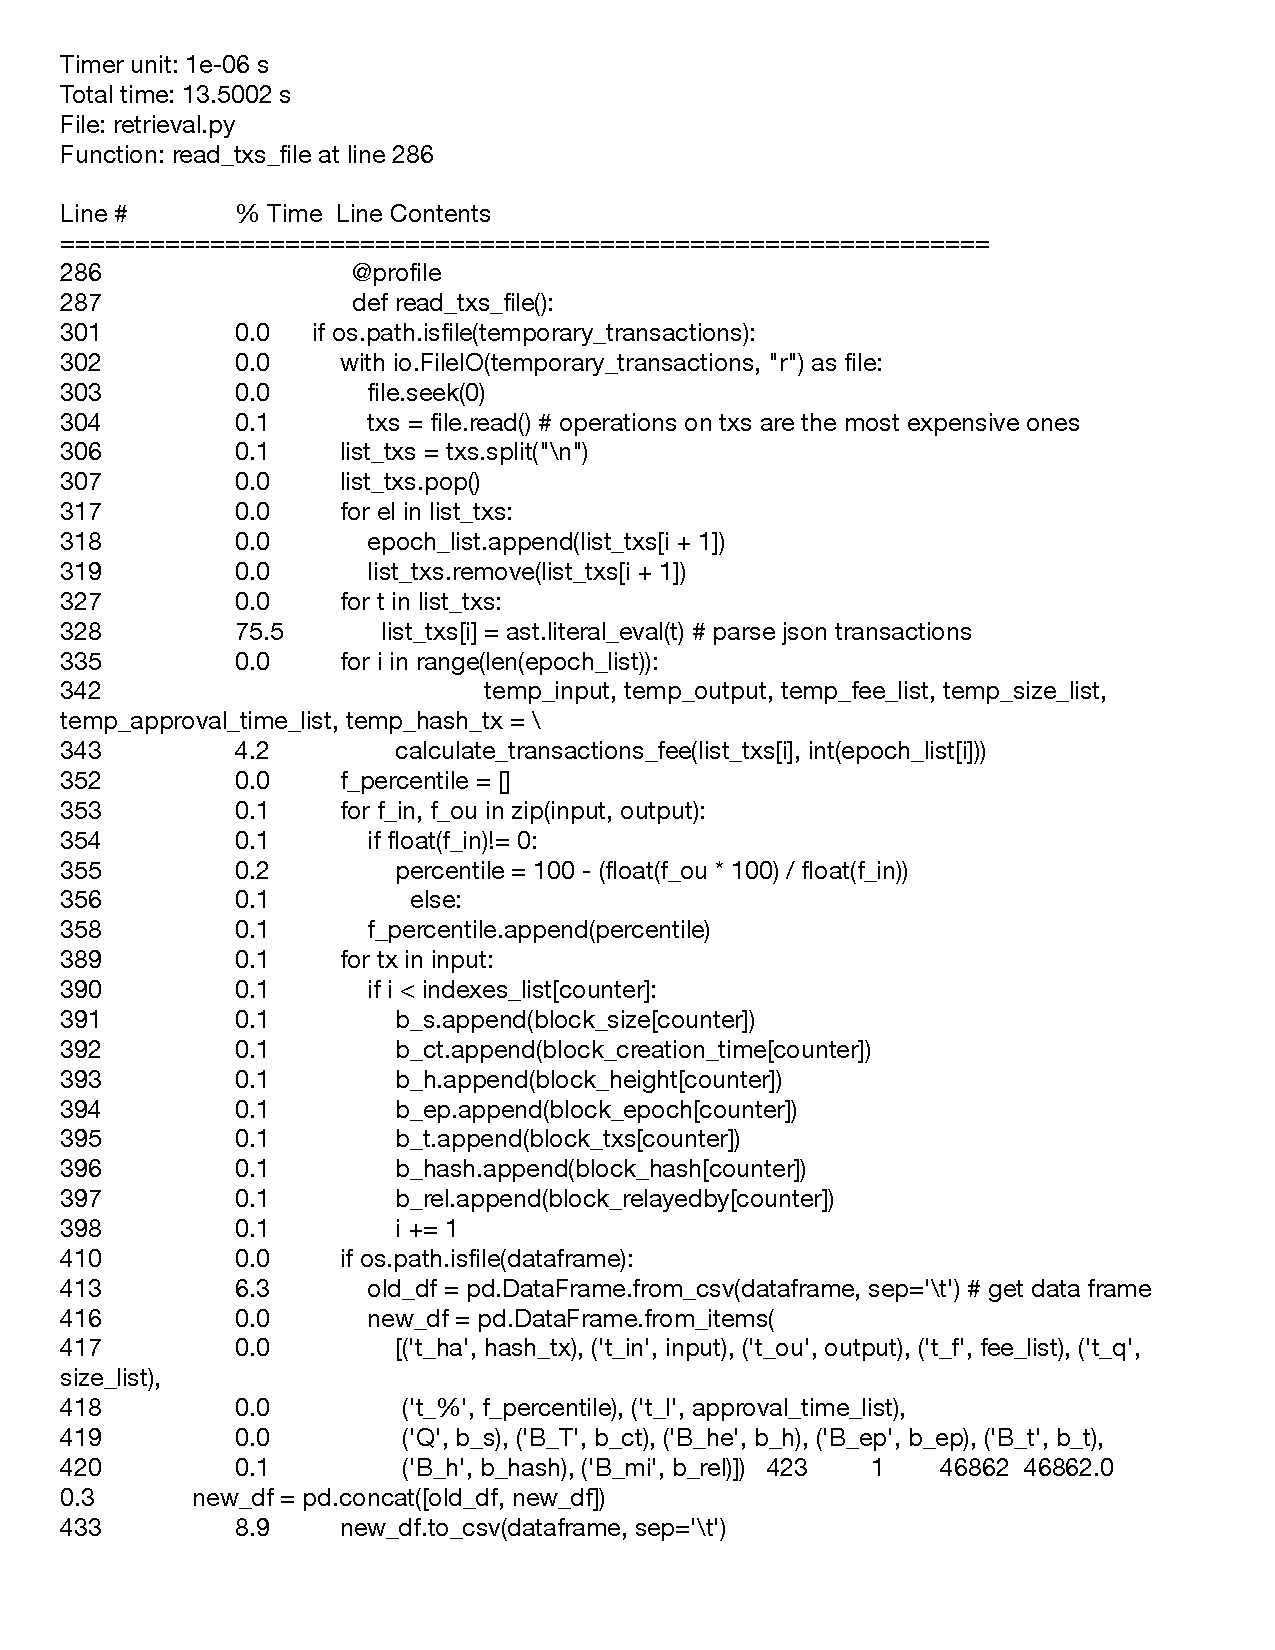
\includepdf[pages=-]{img/read_txs_profile.pdf}
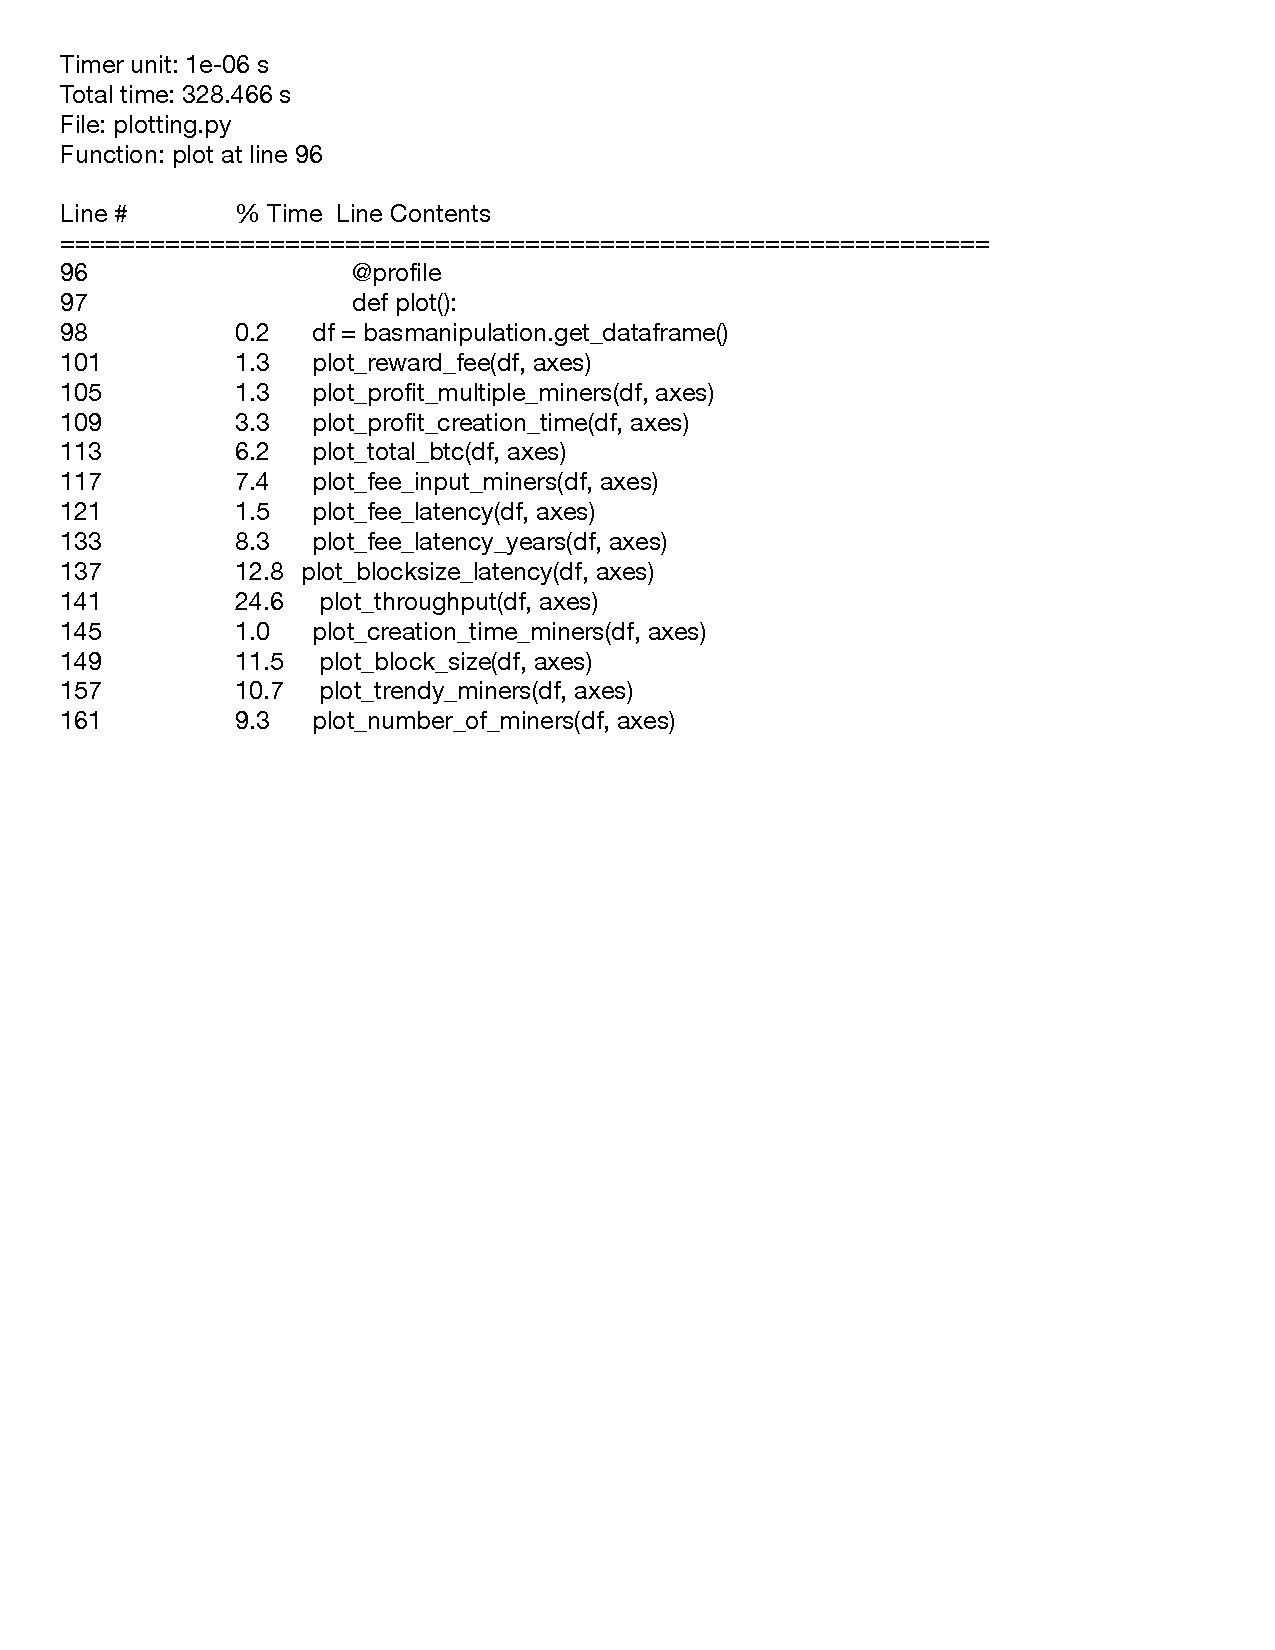
\includepdf[pages=-]{img/plot_profile.pdf}



\chapter{Usage}
\label{app:usage}
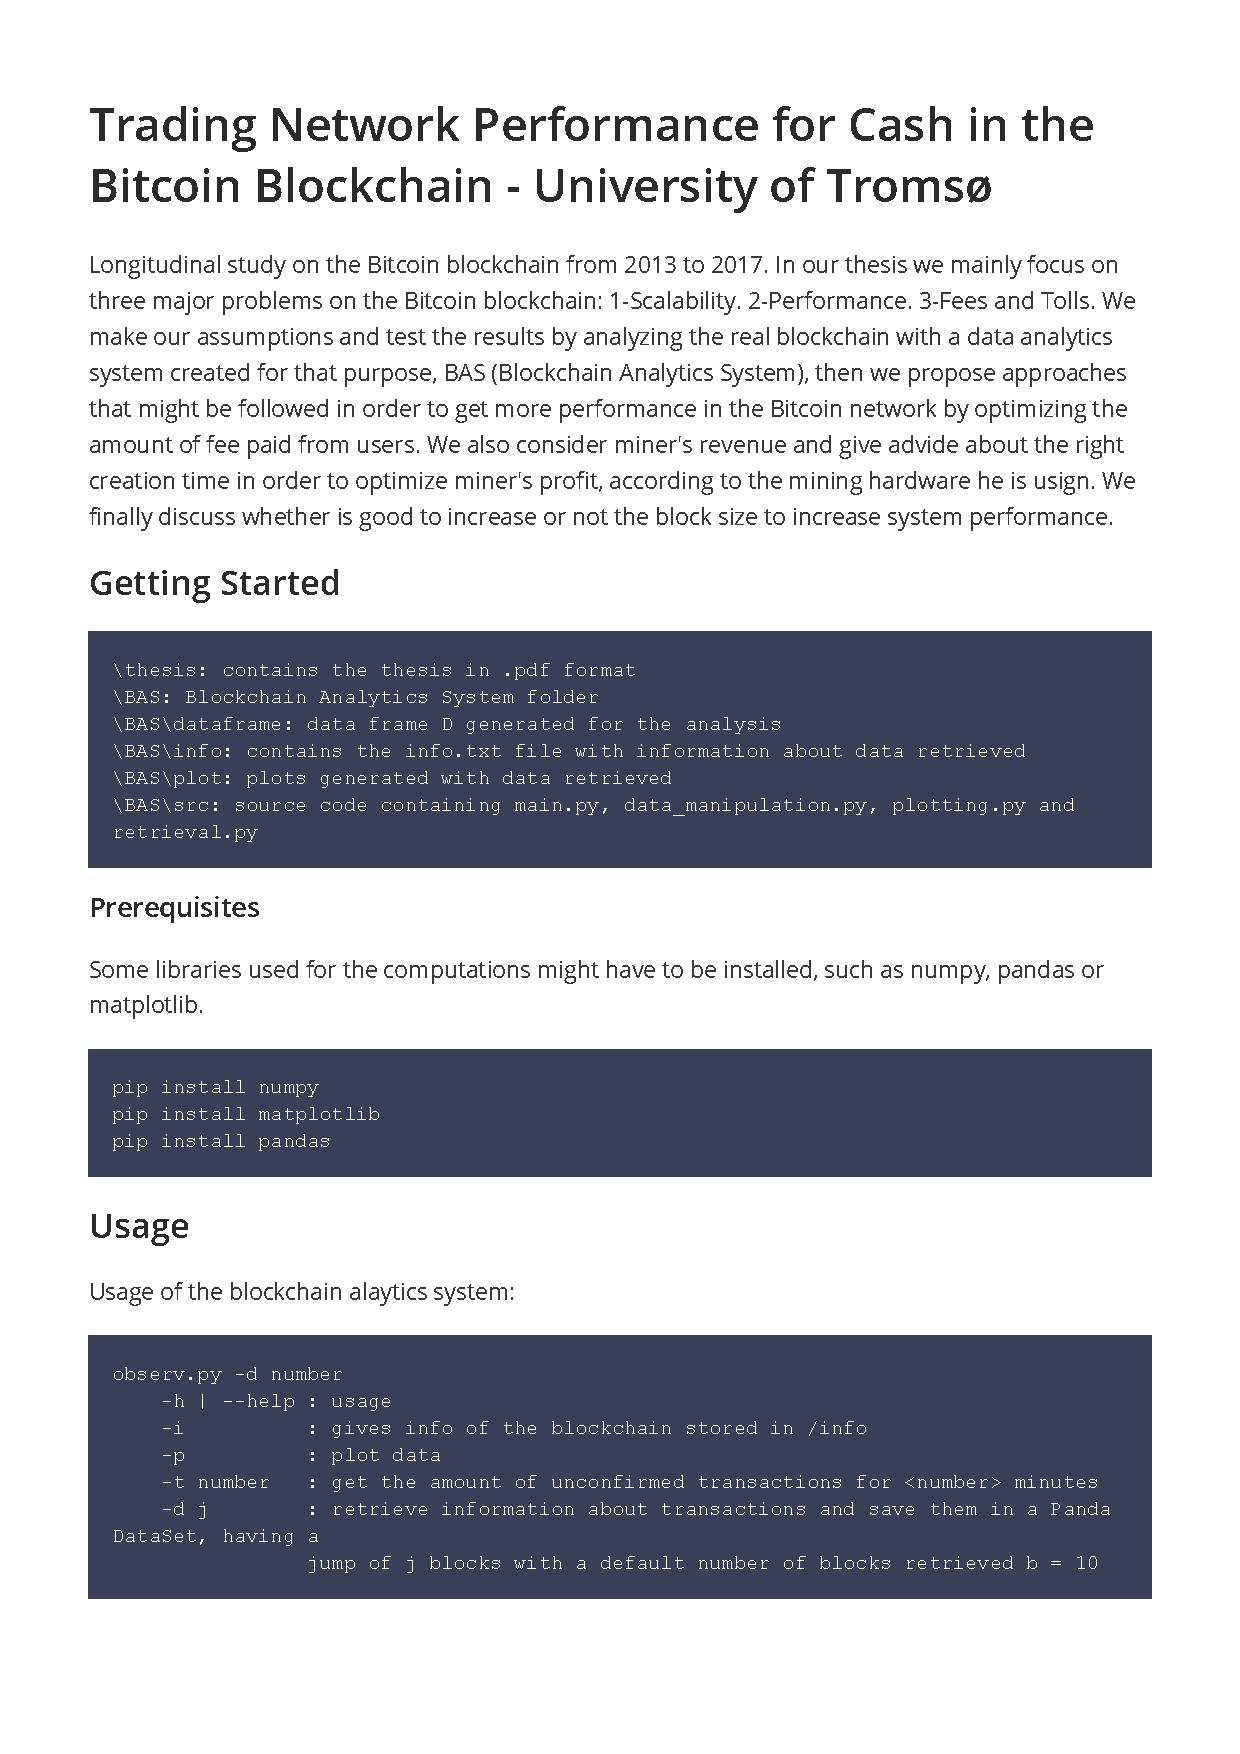
\includepdf[pages=-]{img/README.pdf}

\end{appendices}



\backmatter

\end{document}


%  LocalWords:  cryptocurrency
